\documentclass[a4paper,12pt]{article}
\usepackage[utf8]{inputenc}
% \usepackage{import}
\usepackage{subfig} 
\usepackage{amsmath}
% \usepackage{subfiles}

\usepackage{units}
\usepackage{wrapfig}
% \usepackage{booktabs}
\usepackage[parfill]{parskip}
\RequirePackage{mathptmx}
% \RequirePackage{ftnright}
\RequirePackage{fancyhdr}
%\RequirePackage{graphicx}
\usepackage[pdftex]{graphicx}
% \usepackage{sidecap}
\RequirePackage{hyperref}
% \usepackage{hyperref}
\usepackage[margin=1.5cm]{geometry}
% \usepackage[margin=2.5cm]{geometry}
\usepackage{caption}
\usepackage{framed}
\usepackage[sort,round]{natbib}
\usepackage{rotating}
\usepackage{tabularx}
\setcounter{secnumdepth}{5}
\usepackage{tikz}
\usetikzlibrary{shapes,arrows}

\numberwithin{equation}{section}
% \usepackage{graphicx}
\usepackage{epstopdf}
\usepackage{graphicx}
\usepackage{subfig}
\usepackage{booktabs}
\usepackage{multirow}
% \usepackage[margin=0pt]{subfig}
 % the subfigure package became obsolete, now use subfig with 
% \subfloat[caption]{\includegraphics...} 
\usepackage[margin=0pt]{caption}
% \captionsetup[figure]{width=.85\textwidth}
% \captionsetup[subfigure]{margin=0pt}
% \captionsetup[subfloat]{margin=0pt}
% \usepackage{subcaption}
% \usepackage[margin=0pt]{subfig}
% \includeonly{}

%opening
\title{}
\author{}

% \newcommand*{\refname}{Bibliography}
\begin{document}

\maketitle

\begin{abstract}

\end{abstract}

\section{Introduction}
This study examines the contribution of transient sources to the astrophysical
neutrino flux measured by IceCube (HESE flux). The special focus will be
placed upon Gamma Ray Bursts (GRBs). 

Contrary to most studies which use external GRB triggers from satellites like
Swift and Fermi, this result is based on the opposite idea of using neutrinos
to trigger follow-up observations with Swift and optical telescopes. The
disadvantage of this approach is the additional background while the advantage
is the $2\pi$ field of view (FoV) (northern sky only) and the independence of 
any
gamma-ray sensitivity of the satellites.
Instead of using real measured GRBs, a Toy Monte Carlo was written to simulate
the neutrino flux from a GRB population up to a redshift of eight. The GRB
population and luminosity function is mainly based on a model by Wanderman and
Piran (section \ref{sec:GRB_models}). Other models are included to study the
model dependency.

The neutrino signal will be studied on the level of the Optical- and X-Ray
Follow Up - O(X)FU - and compared to the measured data. The OFU is described
in more detail in section \ref{sec:OFU}. 

The GRB population model, simulated GRB neutrinos and experimental results will
be combined within the analysis frame work of the GRB population Toy Monte
Carlo. It is explained in more detail in section \ref{sec:GRBTMC} while the main
results are summarized and discussed in section \ref{sec:Results}.
\section{Optical- and X-Ray Follow Up}
\label{sec:OFU}
The analysis is based on data from the X-Ray Follow Up including the seasons 
IC86-1 to IC86-3. It is a system that analyzes data at the South Pole, 
searching for multiple neutrinos within 100 seconds from one direction (and a 
possible source 
location) to trigger Follow-Up observations with various telescopes including 
the XRT on board the Swift satellite. The latency of such triggers is about 
three minutes on average. The X-ray Follow-Up (XFU) is a subsystem of the 
Optical Follow-Up (OFU).

\subsection{Alert System}
\label{sec:OFU_alert_system}

Triggered events are reconstructed at the Pole and evaluated at various levels. 
They are first roughly classified as possible muons by the Muon Filter 
($\sim$40 Hz). Stricter cuts are applied on the OnlineL2Filter, to filter 
out badly reconstructed events achieving a rate of about 5 Hz. The lower rate 
allows for further, more detailed reconstructions which are then used for the 
OFU filter. 

The OFU filter is applied to select well reconstructed muon neutrino events 
from the northern sky. Depending on the season a purity of atmospheric 
neutrinos of up to 90\% was 
achieved. The filter was improved season to season though the OFU seasons do 
not match the IceCube seasons. In the first year with the full detector 
configuration (IC86-1), the OFU system was shut down for several month as the 
OFU filter didn't work as expected. The debugging took a long time due to 
multiple software changes that were introduced for IC86-1. For the third OFU 
season in this analysis a boosted decision tree (BDT) was introduced during the 
second full IceCube season (IC86-2). As no changes were introduced for IC86-3, 
the BDT season encompasses the end of IC86-2 and the full IC86-3 IceCube 
season. The first and last runs of all seasons are listed in Table 
\ref{tab:ofu_seasons}.

\begin{table}[h]
  \centering
  \begin{tabular}{l||c|c|c}
   Season & IC86-1 & IC86-2 & IC86-BDT \\
\hline
   first run & 118691  & 120156  & 121788  \\
   start date & 2011-09-16 & 2012-05-15 & 2013-02-01\\
\hline
   last run  & 120155 & 121787 & 124701 \\
   end date & 2012-05-15  & 2013-02-01 & 2014-05-06 \\
  \end{tabular}
  \caption{The table lists the different seasons that were analyzed for this 
work.}
  \label{tab:ofu_seasons}
\end{table}

The OFU cut selection for the IC86-1 and IC86-2 seasons are based on the 
following logic
\begin{equation}
\begin{align}
Zenith (MPE) \geq 90^\circ \; \; and \; \; \frac{logl (MuonLLh)}{NCh - 3.5} & 
<= 8 \; \; and \\ \text{min} (Zenith_{Split}) &\geq 69.51^\circ \; 
\; and \\
((NDir (MPE) \geq 6 \; \;
and LDir (MPE) \geq 280 )& \; \;or \; \;(MuE (MPE) \geq 1e6))
\end{align}
\end{equation}

The $Zenith_{Split}$ values refer to the 
zenith values derived from the topological and time splitter of the events. MPE 
and MuonLLh refer to the different fit types used to extract the parameters. 
The cut scheme was completely reworked  for IC86-BDT to use a BDT cut.
% (reference ???). 

The single neutrino events passing these cuts are further analyzed to search 
for multiplets with multiplets consisting of at least two events arriving 
within the time frame $\Delta t$ and an angular difference $\Delta \Psi$:
\begin{equation}
 \Delta T \leq 100 \text{ s} \;\;\; and \;\;\; \Delta \Psi \leq 3.5^\circ
\end{equation}

All seasons have in common that roughly 50 - 60  doublets per 
year are expected to be generated purely from the background of atmospheric 
neutrinos while the background of higher multiplets (triplets, quadruplets) is 
negligible in the order of once every 15 to 20 years. As observation time with 
the Swift satellite is precious, it was agreed to send only the seven most 
promising doublets looking like a signal per year. The evaluation is based on 
the OFU test 
statistic (OFUtst)
\begin{align}
    \begin{split}
    \lambda = -2 \ln \mathcal{L} &= \frac{\Delta\Psi^2}{\sigma_q^2} + 2 \ln(2
\pi \sigma_q^2) \\
                              &- 2 \ln\left( 1 -
e^{\frac{-\theta_A^2}{2\sigma_w^2}}\right) 
                              + 2 \ln\left( \frac{\Delta T}{\unit[100]{s}}
\right)
    \end{split}
  \label{eq:alert-llh}
\end{align}
in which the time between the neutrinos in the multiplet is denoted as $\Delta 
T$
and their angular separation as $\Delta\Psi$. $\sigma_q^2 = \sigma_1^2 +
\sigma_2^2$ and $\sigma_w^2 = \left(1/\sigma_1^2 + 1/\sigma_2^2\right)^{-1}$
 are the combined uncertainties of the directional
reconstruction errors $\sigma_1$ and $\sigma_2$ of the two neutrino events.
$\theta_A$ corresponds to the (circularized) angular radius of the field
of view (FoV) of the follow-up telescope (set to $0.5^\circ$ for Swift). A cut 
value $\lambda_\text{cut}$ was chosen each season to filter out the best nine 
alerts (Table \ref{tab:llh cut values}). The value change with the IC86-BDT 
season as a higher singlet rate was allowed resulting in more doublets per 
year. Statistically, two more alerts will be 
lost because Swift can't observe about 80\% of the sky due to the moon and the 
sun.

\begin{table}[h]
  \centering
  \begin{tabular}{l|c|c|c}
   Season & IC86-1 & IC86-2 & IC86-BDT \\
\hline
   cut value & -8.8  & -8.8 & -9.41 \\
  \end{tabular}
  \caption{The cut values on the likelihood to filter down the number of
background doublets to less or equal than 9.}
  \label{tab:llh cut values}
\end{table}
The full derivation of the test statistic can be found in the proposal to the 
IceCube collaboration (reference ???).


\subsection{Monitoring}
The alert system described in the previous section delivers alerts only if it 
is operational. To monitor the system an additional kind of alerts were 
introduced.
Test 
alerts are multiplets formed by neutrino events with a time 
difference of less than 100 seconds and an angular difference of $3.5 < \Delta 
\Psi \leq 7.5^\circ$. The events going into the multiplet decision have been 
selected by applying softer cuts on the Online Level 2 events, i.e. they are 
more background contaminated than the OFU events. The less stringent cuts and 
the different condition for the angular difference yield the desired test alert 
rate of about one test alert every ten minutes and prevent test alerts to be 
alerts as well. A lack of test alerts indicates problems with either the 
IceCube detector itself, our alert system, or the communication processes and 
an 
alarm is raised after a two hour signal silence.
\section{Background Expectation}
The previous section described the set up of the X-ray Follow-Up including the 
expectation of generating alerts based on background events. It is 
crucial to understand the amount of the false positives to distinguish a 
possible signal contribution to the alert rate. An average background 
estimation is obtained by scrambling the neutrino singlets on the level of the 
Optical Follow-Up Filter.

The neutrino singlets on the level of the Optical Follow-Up Filter consist of 
about 80 - 90\% 
% (???) 
of atmospheric neutrinos and 10 - 20\% of 
misreconstructed muons. If a signal is present, it will be suppressed  in 
comparison to the background. 
In the scrambling process the time and reconstruction information are split. 
While the time structure of the events is being kept in tact, incorporating 
possible time dependent rate changes, e.g. due to seasonal variations, for each 
scrambled result, the reconstruction information such as direction and quality 
is stripped of and randomly attributed to a different event time. An 
illustration is shown in Figure \ref{fig:scrambling_illustration}.
\begin{figure}[h]
 \centering
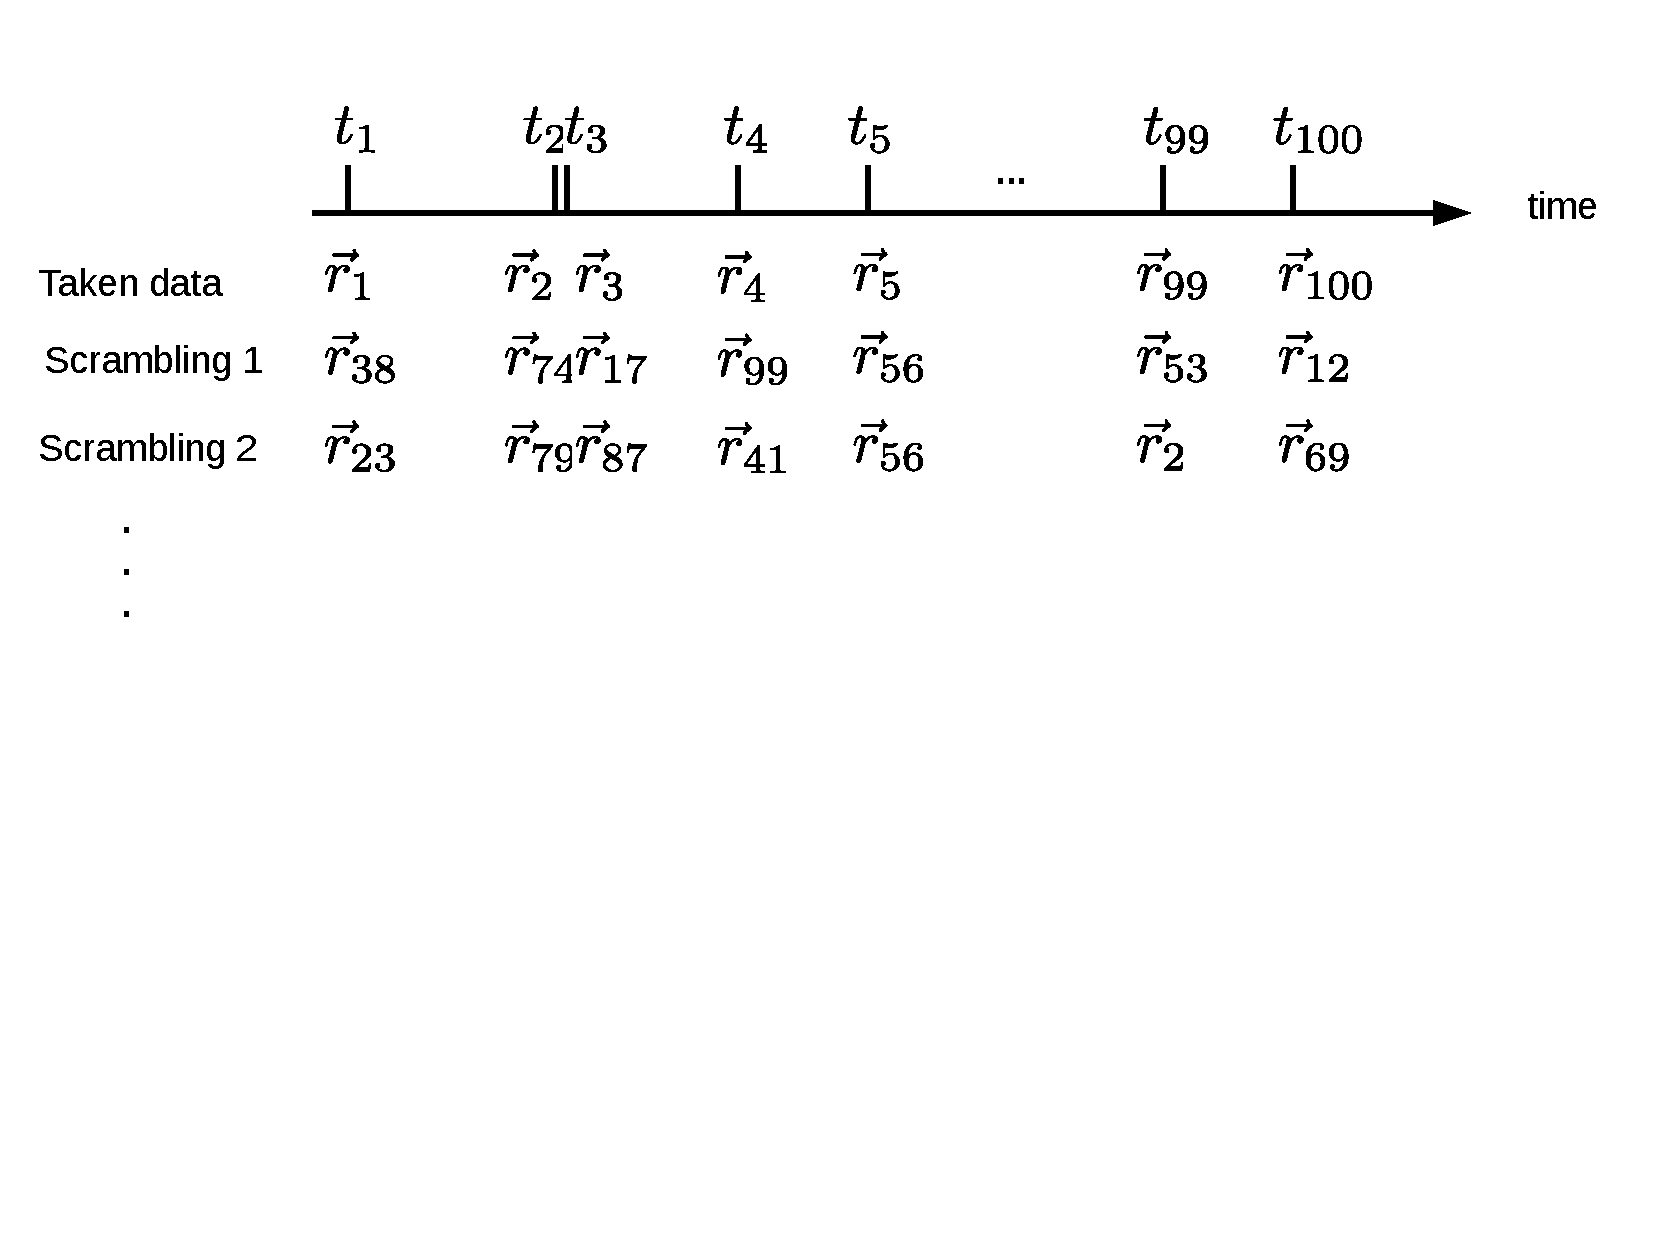
\includegraphics[trim=0cm 10.5cm 1cm 
1cm,clip=true,width=0.65\textwidth]{fig/scrambling_illustration.pdf}
\caption{An illustration of the scrambling process for an example of 100 
events. The time structure stays the same while the directional information is 
appointed to a new time randomly with each scrambling.}
\label{fig:scrambling_illustration}
\end{figure}

Events considered in the background estimation should only be events that 
actually were able to contribute to the triggered alerts, i.e. events detected 
while the Follow-Up system was operational. Towards that end all OFU singlets 
were extracted from the database and a time filter 
developed to exclude events happening during the Follow-Up downtime.
% There can be several reasons that have to be included in the filter. 
There are several factors contributing to downtime.
Only data 
taken during good physics runs are considered. The good-run decision is based 
on a goodrun list extracted from i3live. The snapshot numbers are listed in 
 Table \ref{tab:goodrunlists}.

\begin{table}[h]
  \centering
  \begin{tabular}{l||c|c|c}
  Season & IC86-1 & IC86-2 & IC86-3 \\
  \hline
  snapshot & 94 & 109 & 93 \\
  \end{tabular}
  \caption{The snapshot numbers of the goodrun lists used for the different 
seasons.}
  \label{tab:goodrunlists}
\end{table}
Any real alert that was triggered during the three years considered in this 
analysis that occurred during a bad run is excluded in this analysis.

However, the good run list only evaluates the normal function of the IceCube 
detector but does not include downtime that is isolated to the Follow-Up 
System. Reasons can be various from software problems only affecting the OFU 
system to transmission problems via the ITS satellite.

\begin{table}[h]
  \centering
  \begin{tabular}{l|c|c|c}
   Season & IC86-1 & IC86-2 & IC86-BDT \\
\hline
   livetime [d] & 233.56 & 235.42 & 407.38 \\
   uptime [\%] & 0.91 & 0.90 & 0.89 \\
\hline
   expected Swift & 5.42 & 6.49 & 5.7 \\
   measured Swift & 6 & 5 &  7 \\
\hline
   expected multiplets & 0.044 & 0.063 &  0.073 \\
   measured multiplets & 0 & 0 & 0 \\
  \end{tabular}
  \caption{The table lists both the uptime of the Optical Follow-Up system and 
the results of the data scrambling to estimate the average background rate. The 
measured values are documented here for comparison.%rms values?
}
  \label{tab:scrambling_results}
\end{table}
The OFU uptime is 
evaluated using the test alerts that are designed to monitor the OFU systems.
On average, a test alert is expected to arrive every ten minutes. For this 
analysis, the system is considered 'down' if there is no test alert in a 
window twenty minutes after a test alert and twenty minutes before the next 
alert. This procedure averages over the effects that the system might crash 
directly after a test alert or that a new test alert arrives directly after the 
restart of the system and that the system is running though no test alerts 
arrived for over twenty minutes.

Using this time mask, all online alerts could be reproduced by re-analyzing the 
data offline and no new alerts were found. On average, 5.4, 6.5 and 5.7 Swift 
doublets were expected during the different seasons while the higher multiplet 
rate expectation varies between 0.044 and 0.073 (Table 
\ref{tab:scrambling_results}). An example of the scrambled distributions of 
expected Swift alerts during the IC86-1 season can be seen in Figures
\ref{fig:swift_scrambling} and \ref{fig:swift_scrambling_cum}.

The OFU system had an average uptime of 90\%. 
This includes downtime for OFU unrelated reasons like calibration runs.

\begin{figure}[h]
\centering
 \captionsetup{width=.9\textwidth}
%  \captionsetup{margin=0pt}
\subfloat[The differential distribution \label{fig:swift_scrambling}]{%
 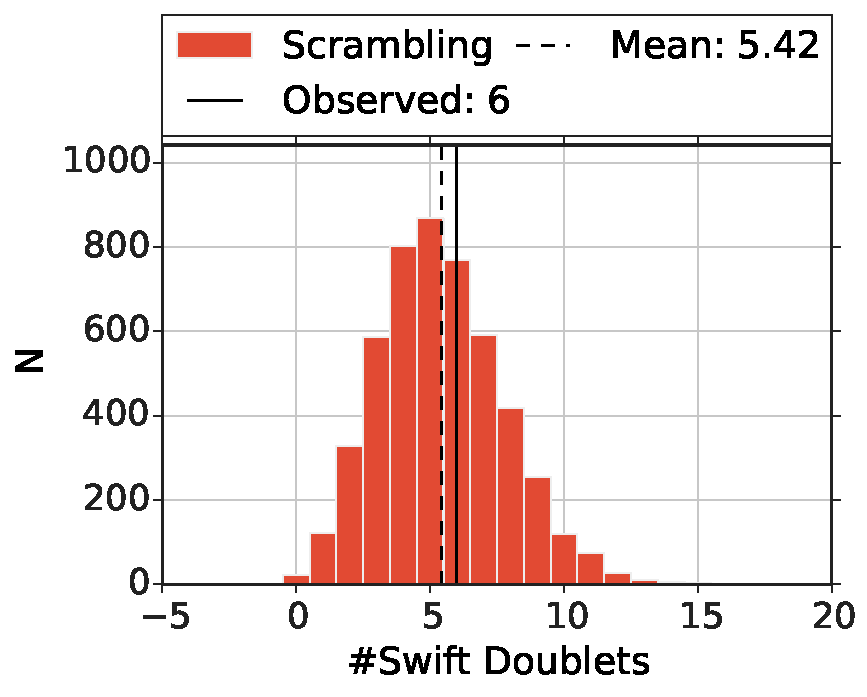
\includegraphics[width=0.45\textwidth]{fig/swift_scrambling.pdf}}
 \subfloat[The inverse cumulative distribution.
\label{fig:swift_scrambling_cum}]{%
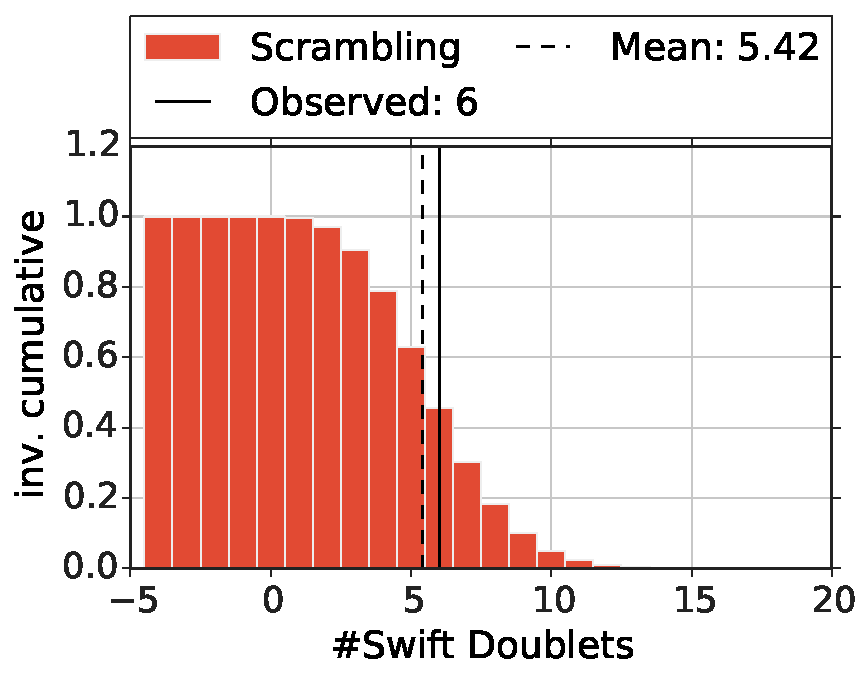
\includegraphics[width=0.45\textwidth]{fig/swift_scrambling_cum.pdf}}
\caption{The differential and inverse cumulative distributions of 
detectable Swift doublets for a hundred thousand scrambled datasets. The 
distributions for 
IC86-1 is chosen as an example.}
\end{figure}



% error on livetime and mean value in an example? like decrease to 10 min? and 
% increase to 30 min?
% 
% table with uptime and mean values. quadruplets?
% 
% plots for three seasons? or is one season enough?
% 
% split the table up. part into Optical Follow-Up filter part into results. 
% though the p-values are not calculated according to the significance section. 
% livetime/uptime doesn't fit for IC86-1
% \begin{table}[h]
%   \centering
%   \begin{tabular}{l|c|c|c}
%    Season & IC86-1 & IC86-2 & IC86-BDT \\
% \hline
%    livetime [d] & 233.56 & 235.42 & 407.38 \\
%    uptime [\%] & 0.96 & 0.90 & 0.89 \\
% \hline
%    expected Swift & 5.42 & 6.49 & 5.7 \\
%    measured Swift & 6 & 5 &  7 \\
%    p value & 0.45 &  0.79 & 0.34 \\
% \hline
%    expected multiplets & 0.044 & 0.063 &  0.073 \\
%    measured multiplets & 0 & 0 & 0 \\
%    p value & 1 & 1 & 1\\
%   \end{tabular}
%   \caption{}
%   \label{tab:scrambling_results}
% \end{table}
\section{GRB models}
\label{sec:GRB_models}
Most GRB analysis within IceCube use information from observed GRBs to look
for neutrino clusters in time and space correlation with the detected GRBs.
This strategy has the obvious advantage of reducing the neutrino background to
achieve higher significance per GRB observation. However, due to the limited
Field of View of the satellites there will be many GRBs that stay undetected.
Furthermore, one is biased by the detection sensitivity of the satellites.

In this analysis, a GRB population is assumed based on theoretical work and
extrapolation based on data from Swift and other satellites. The redshift and
luminosity functions are extracted.
The neutrino luminosity function is assumed to have the same shape and is
shifted in energy by an efficiency factor $\epsilon$ (see section ???).
%  to calculate their
% expected signal in IceCube.
The different population models under consideration are discussed in this
chapter.

The main analysis has been done based on the luminosity function and GRB rate
density calculated by Wanderman and Piran (\ref{ssec:WP}). 
The other models presented here were considered to examine the dependency on
the assumed model.

\subsection{Cosmology}
The following cosmological definitions are used in the further calculations.

\textbf{Differential co-moving shell volume} 
\begin{equation}
dV = 4 \pi D_H \frac{(1+z)^2D_a^2(z)}{K(z)}dz
\end{equation}
\textbf{Hubble distance}
\begin{equation}
 D_H = \frac{c}{H_0} = 3000 h^{-1}\text{Mpc}
\end{equation}
\textbf{Angular distance}
\begin{equation}
 D_a(z) = (1+z)^{-2} D_l(z)
\end{equation}
\textbf{Parameters} 
\begin{itemize}
  \item  $K(z) = \sqrt{\Omega_m (1 + z)^3 + \Omega_{\Lambda}}$
 \item $h=0.7$
 \item $\Omega_m = 0.3$
 \item $\Omega_\Lambda$
\end{itemize}

\subsection{Wanderman Piran}
\label{ssec:WP}
Wanderman and Piran \cite{WP} extracted a GRB distribution in redshift and
luminosity using GRB data up to 2009 applying detection efficiencies for
both the detection in $\gamma$- rays and a following determination of the host
redshift, i.e., the redshift of the GRB. 

The differential co-moving rate of bursts (fig. \ref{fig:GRB_rate_density}) at a
redshift $z$ is
\begin{equation}
 R(z) = \frac{R_{\text{GRB}}(z)}{(1+z)} \frac{dV(z)}{dz}
 \label{eq:Rz}
\end{equation}
$dV(z)/dz$ is the differential co-moving shell volume 
and the factor $(1+z)^{-1}$ reflects the cosmological time dilation.
$R_{\text{GRB}}$ is fitted to data with the result (Fig \ref{fig:RGRB})
\begin{equation}
\label{eq:R_z}
    R_{\text{GRB}}(z) = \begin{cases}
                        \rho_0 \cdot (1 + z)^{n_1} & z \leq z_1 \\
			 \rho_0 \cdot (1 + z_1)^{n_1 - n_2}(1 + z)^{n_2} & z >
z_1
                        \end{cases}
\end{equation}
with
$n_1= 2.07$, $n_2=-1.36$, $z_1=3.11$ and the local rate $\rho_0=1.25
\text{Gpc}^{-3} \text{yr}^{-1}$.

% 1.25 \cdot 10^{-9} \cdot \text{Mpc}^{-3} \cdot \text{yr}^{-1}$

\begin{figure}[h]
\centering
 \captionsetup{width=.9\textwidth}
%  \captionsetup{margin=0pt}
\subfloat[Derived RGRB function (WP)\label{fig:RGRB}]{%
 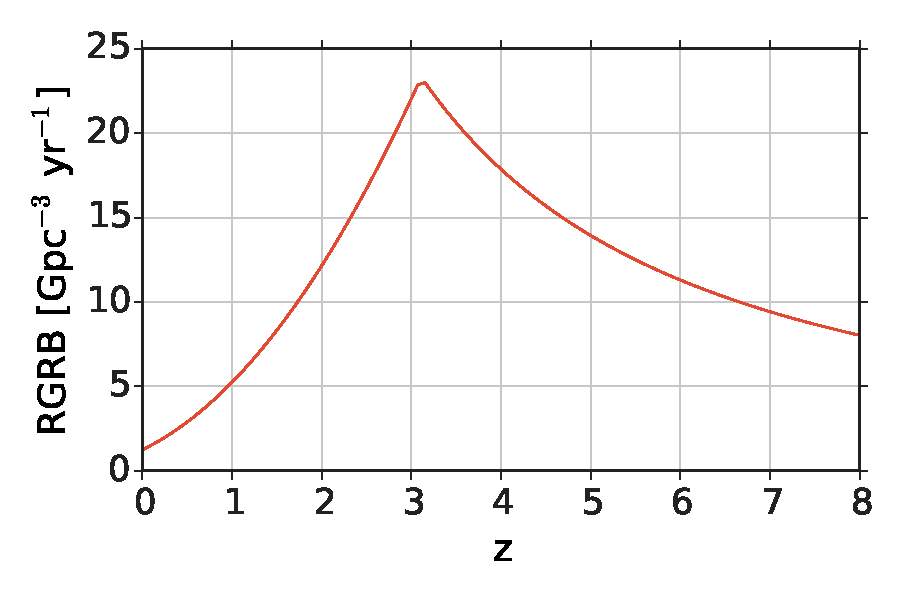
\includegraphics[width=0.45\textwidth]{fig/RGRB_WP.pdf}}
 \subfloat[Differential co-moving rate\label{fig:GRB_rate_density}]{%
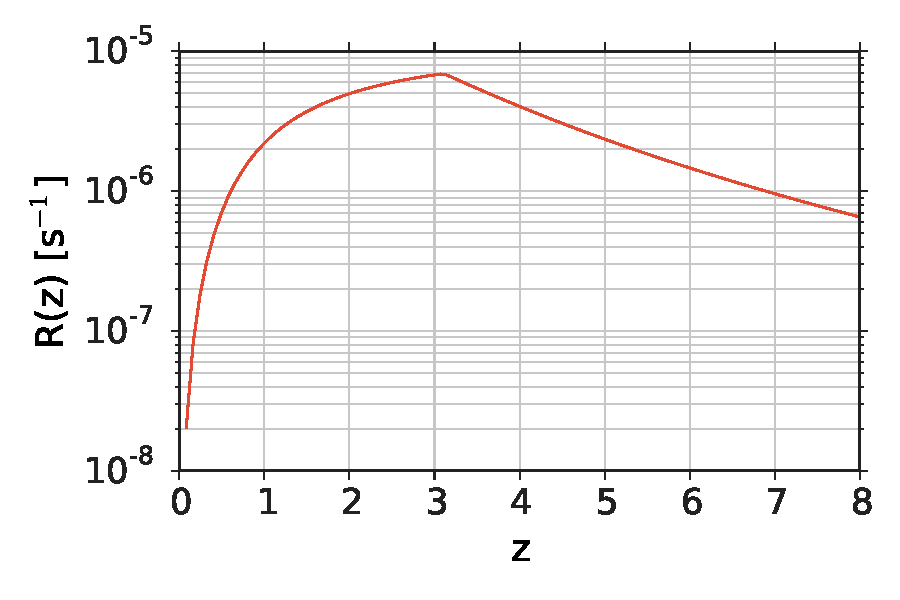
\includegraphics[width=0.45\textwidth]{fig/Rz_WP.pdf}}
\caption{The distribution of GRBs over the redshift displaying the derived RGRB 
function and the differential co-moving rate.}
\end{figure}




The peak $\gamma$-luminosity at the source
$L_{\text{Peak}}$ (Fig. \ref{fig:Lpeak})  is determined to follow
\begin{equation}
\label{eq:Phi_L}
 \Phi(L_{\text{Peak}}) = \begin{cases}
      \left(\frac{L}{L_{*}} \right)^{-\alpha} &  L < L_{*} \\
      \left(\frac{L}{L_{*}} \right)^{-\beta}  &  L > L_{*}
     \end{cases}
\end{equation}
in which $\text{log}_{10}L_{*}=52.53 \text{ erg / s}$ is the break luminosity
and $\alpha=0.17$ and $\beta=1.44$ are the spectral indices (Table
\ref{tab:grb_model_params}).
No redshift evolution of the luminosity is assumed.
\begin{figure}[h]
% \begin{minipage}{\textwidth}
 \captionsetup{width=.6\textwidth}
 \centering
%  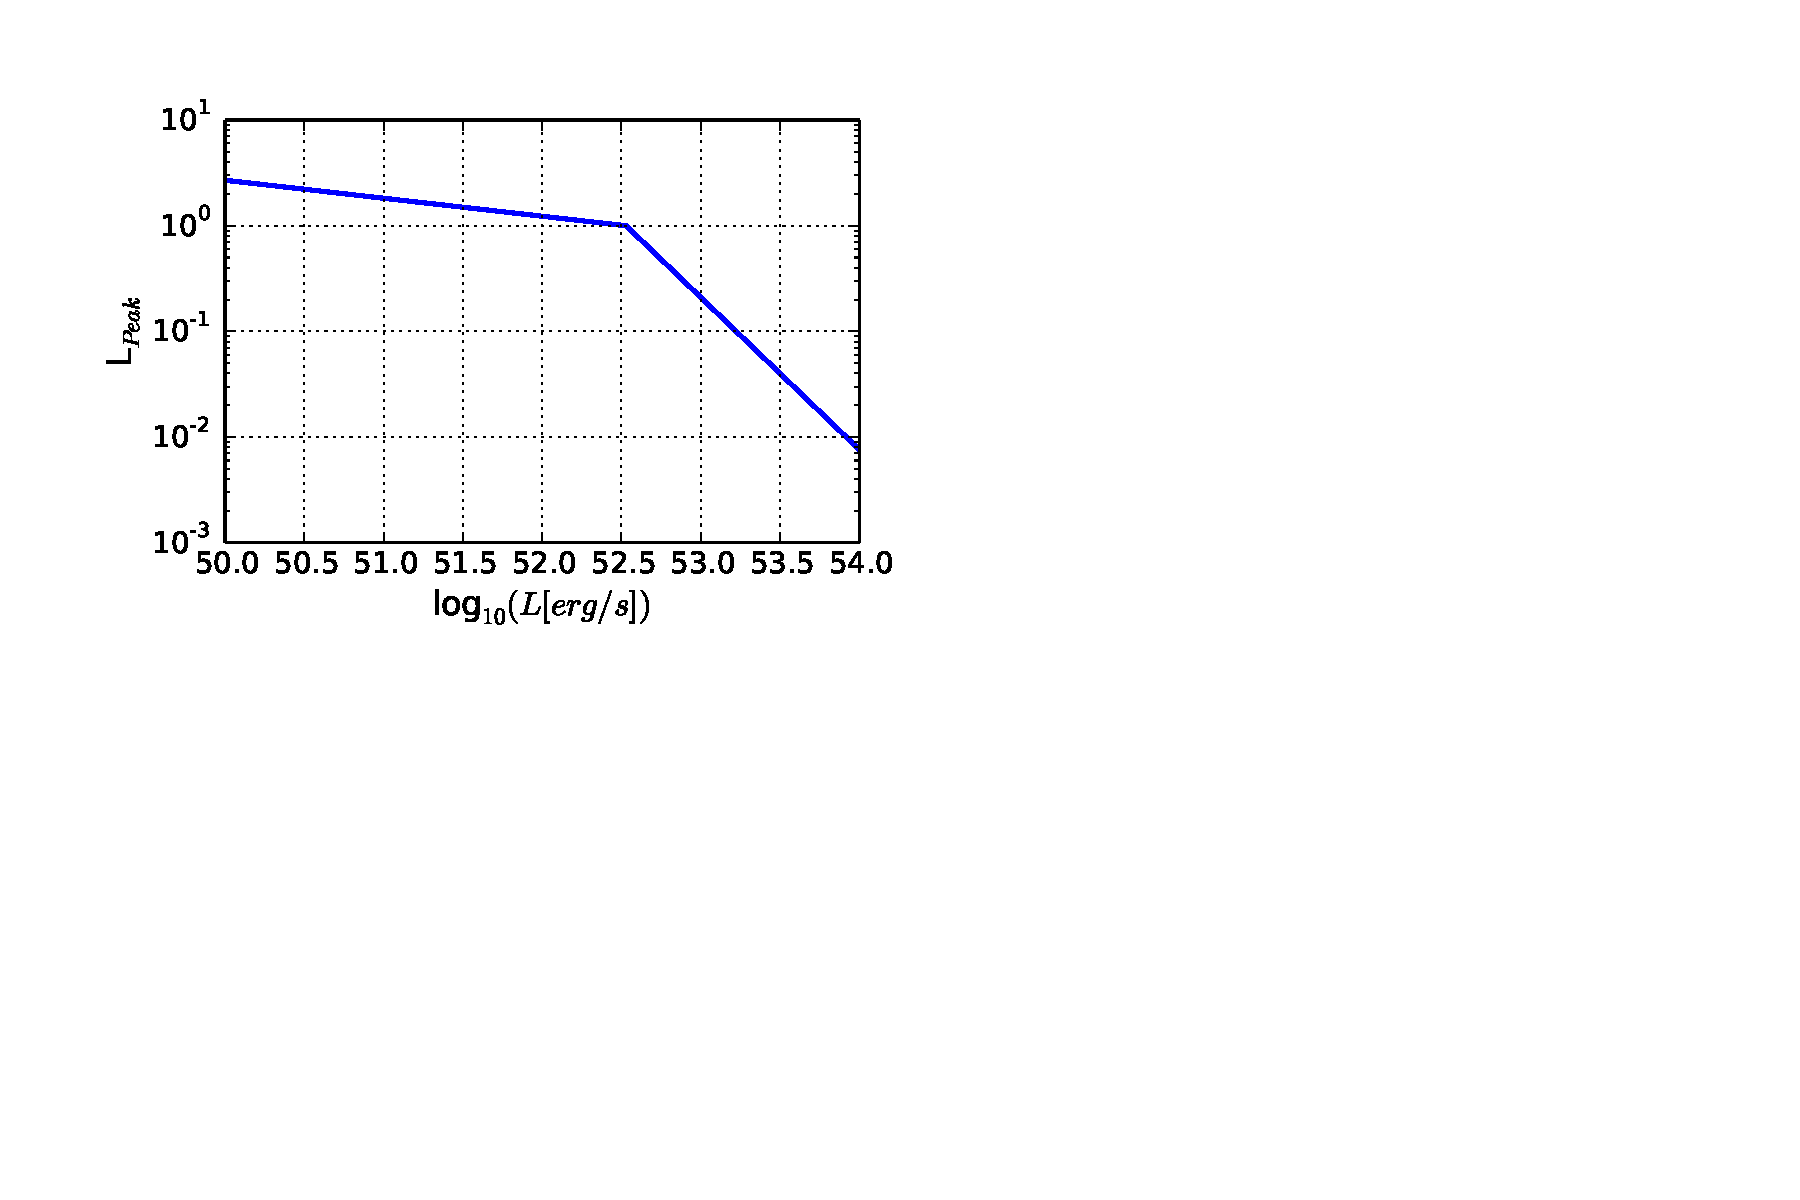
\includegraphics{fig/Lpeak.pdf}
 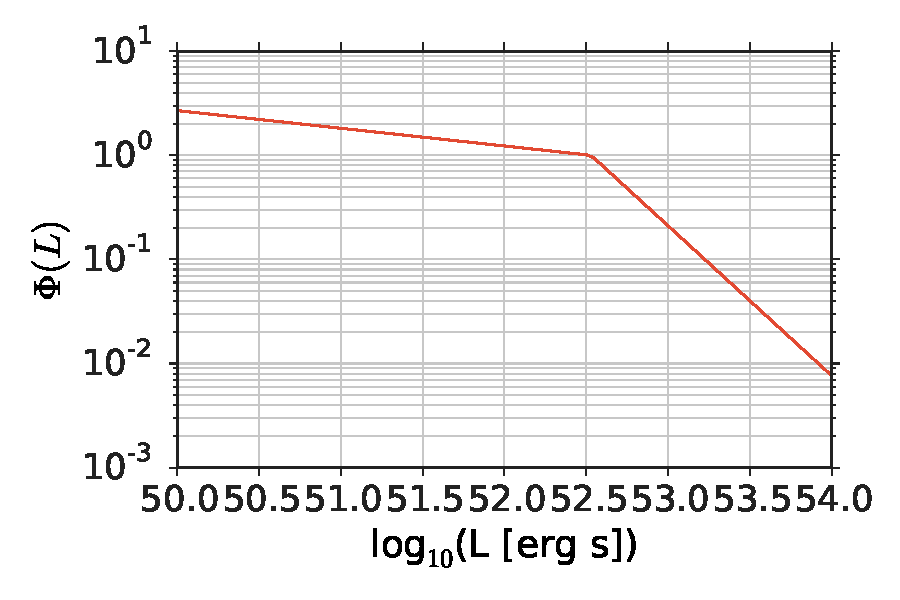
\includegraphics[width=0.6\textwidth]{fig/Lpeak_wp.pdf}
 \caption{The luminosity function derived in the WP model. (deleted this figure 
and use the one including HC?)}
 \label{fig:Lpeak}
% \end{minipage}
\end{figure}
\subsection{Howell Coward}
\begin{table}[h]
  \centering
  \begin{tabular}{l||c|c|c|c|c|c|c|c|c}
    Model & log$_{10}\left(L_* \left[ \text{erg} \text{ s}^{-1} \right] \right)$
& $\alpha$ & $\beta$ & $\rho_0 \left[\text{Gpc}^{-3} \text{ yr}^{-1} \right]$ &
$z_1$ & $n_1$ & $n_2$ & $N_\text{GRB}$ \\
    \hline
    WP & 52.53 & 0.17 & 1.44 & 1.25 & 3.11 & 2.07 & -1.36 & 9082.83\\
%     HC 1 & 51.9 & 0.95 & 2.59 & 0.48 & 3.6 & 2.1 & -0.7 & 4791.97\\
    HC & 51.7 & 0.13 & 2.42 & 0.48 & 3.6 & 2.1 & -0.7 & 4791.97\\
  \end{tabular}
  \caption{Fit parameters to the luminosity functions and redshift
distributions of the tested models.}
  \label{tab:grb_model_params}
\end{table}
There is a more recent work \cite{HC} by Howell, Coward, Stratta,
Gendre and Zhou basing the redshift distribution on
the same general shape as Wanderman Piran and testing various luminosity 
functions. For purposes of
readability it will be called Howell-Coward or HC-model. 
One of the tested luminosity functions
will be compared to the model by Wanderman and
Piran (WP). 
%They are designated HC1 and HC2.

Similarly to Wanderman and Piran, the luminosity is assumed to not evolve
with redshift in their main work.
The same functions as in WP are used for redshift distribution (eq. 
\ref{eq:R_z}) and the
luminosity function (Eq. \ref{eq:Phi_L}), but different fit results
were obtained for the parameters (Table \ref{tab:grb_model_params}).

The considered luminosity range is with $\text{log}_{10} L_\text{Peak} \in
\left( 49, 54 \right)$ larger than in WP ($\text{log}_{10} L_\text{Peak} \in
\left( 50, 54 \right)$). The break peak luminosity is lower
than in WP transitioning into a harder slope towards higher luminosities (Fig.
\ref{fig:wp_hc_comp}). At lower luminosities the slopes of HC and WP are
quite similar (0.13, 0.17) leading to more low luminosity GRBs in HC due to the 
greater range.

% The redshift distribution in HC is shifted to smaller values of $R(z)$ as a
% smaller local rate and total number of GRBs is assumed (Table
% \ref{tab:grb_model_params}). 
The redshift distributions rise to the break redshift quite similarly although 
the break is at higher redshifts (3.6 compared to 3.11) for HC transitioning
into a slower decay at large $z$. The overall impact are more distant GRBs in
HC than in WP which should lead to a slight weakening of the limits.

\begin{figure}[ht]
% [htb] 
\subfloat[Luminosity functions\label{fig:wp_hc_comp_lum}]
{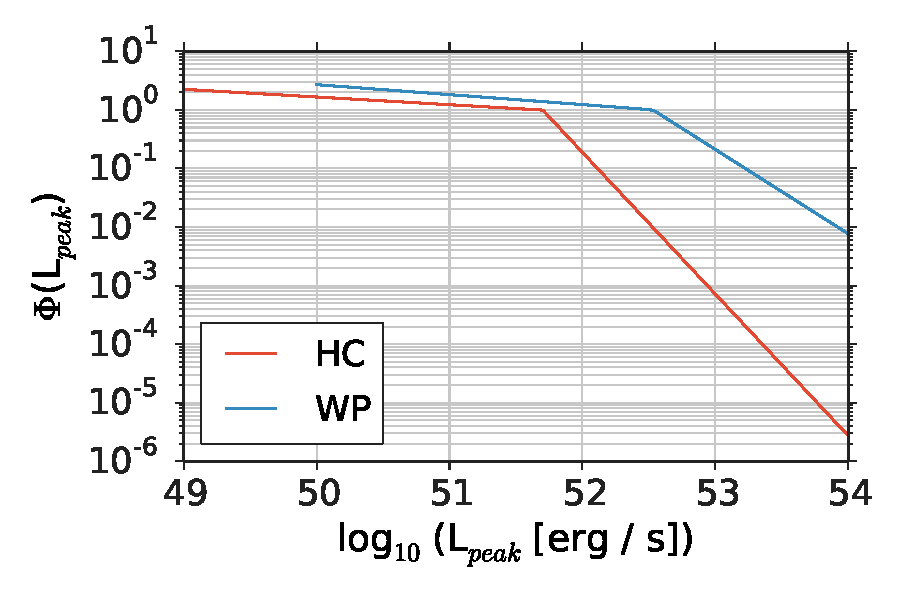
\includegraphics[width=0.48\textwidth]{fig/grb_models_lum_comp_L45.pdf}}
    \hfill
\subfloat[Redshift distributions\label{fig:wp_hc_comp_z}]
{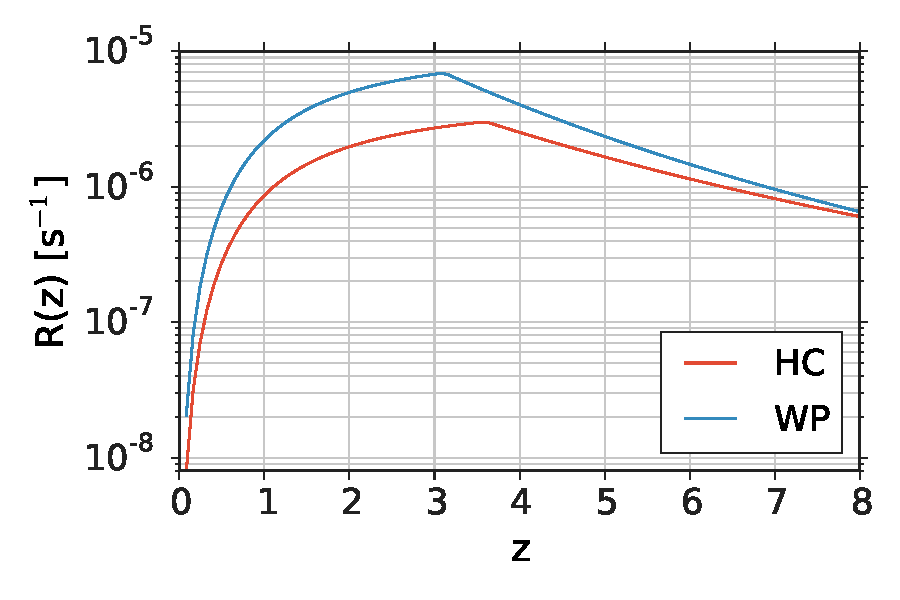
\includegraphics[width=0.48\textwidth]{fig/grb_models_redshift_comp.pdf}}
    \caption{The luminosity functions (left) from the
Wanderman-Piran model and two functions from the HC model on the left. The WP
only take into account luminosities in the range of $10^{50} - 10^{54}$ erg / s
which is reflected in the shorter blue line.\\
The redshift distributions (right) develop similar up to $z=3.11$ at which point
it breaks for the WP-model. The HC predicts more GRBs at higher redshift
values.}
\label{fig:wp_hc_comp}
\end{figure}


% While most of cases discussed in (reference ???) imply independentend luminosity
% and redshift, a correction is given to examine the influence of a possible
% evolution. This will be added at a later point as a third comparison model.
\subsection{Long low luminosity GRBs}
In recent years, IceCube has started to rule out the first optimistic GRB
neutrino emission models leading to new ideas as to possible neutrino emitters.
It has been proposed (reference ???) that a high number of very low
luminosity GRBs exists that are difficult to detect in $\gamma$-rays but could
produce most of the neutrinos expected from GRBs. In principle, the follow-up
analysis based on IceCube triggers can be an approach to examine these objects.
Thus they are mentioned here briefly for completeness sake. 

Unfortunately, these low luminosity GRBs are predicted to have a prompt
emission phase in the range of $10^3$ s. The follow-up program suppresses
background by allowing a maximal time difference of 100s between two events
reducing the sensitivity to very long GRBs at the same time. Therefore, they
have not been examined yet within this analysis but mentioned for the 
interested reader.

\subsection{Supernovae}
The models presented described GRB population models. However, the Optical 
Follow-Up is sensitive to all short ($O(10 \text{ s})$) transient neutrino 
sources. E.g. the simulation can be used to examine a population of core 
collapse SN as well. A model predicting high energy neutrinos from SNe (AB 
reference ???) assumes a jet production withing the SN similar to the jets of 
the GRB fireball model. Due to the lack of energy they do not penetrate the 
stellar envelope and are therefore invisible due the telescopes 
observing the electromagnetic signal. In contrast, neutrinos would escape the 
SN and could possibly be detected within IceCube. The exact mechanism and 
resulting predicted spectrum is not important for this analysis as we assume a 
population of sources and attribute them a spectrum that reproduces the 
measured HESE flux.
%Nora s work

SNe follow the star formation rate which, in first order, can be approximated 
by the Wanderman Piran redshift distribution. However, the luminosity function 
differs quite a bit by not showing the big variations in luminosity that are 
observed for GRBs. Instead, the luminosity function is assumed to follow a 
Gaussian curve in logarithmic space with a width of 0.4 orders of magnitudes 
corresponding to a width of one astronomical magnitude. A comparison to the WP 
luminosity function is shown in Figure \ref{fig:lum_SN}. The mean luminosity is 
chosen at random and will be later adjusted to create the expected neutrino 
flux (Section ???).


\begin{figure}
 \centering
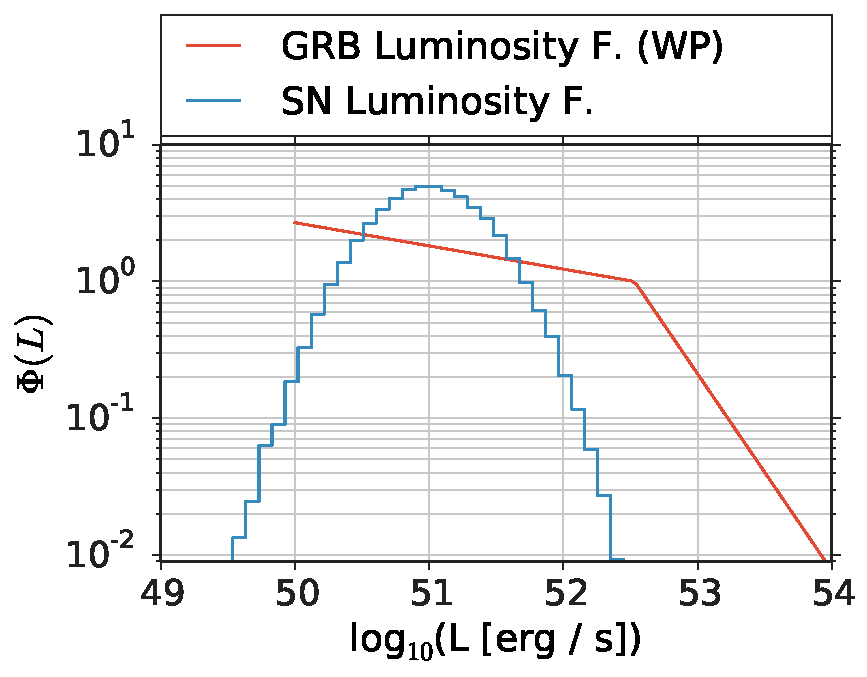
\includegraphics[width=0.65\textwidth]{fig/Lpeak_wp_SN.pdf}
\caption{}
\label{fig:lum_SN}
\end{figure}


\subsection{T90}
\begin{figure}[ht]
\centering
 \captionsetup{width=.68\textwidth}
{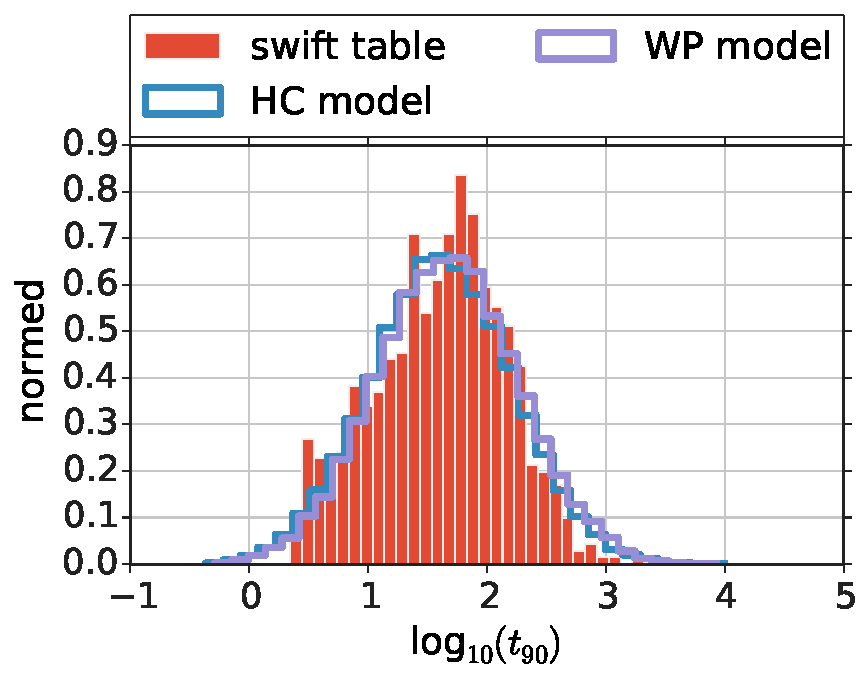
\includegraphics[width=0.68\textwidth]{fig/t90earth.pdf}}
    \caption{The $t_{90}$ distributions at earth based on data extracted from
the Swift database (reference ???) and the drawn distributions based on
$t_{90}$ values drawn at source and folded with the redshift distributions.}
\label{fig:t90earth}
\end{figure}
Ninety percent of the detectable $\gamma$-ray flux is received between a
time intervall called $t_{90}$. Reference (???) lists values for most GRBs.
The extracted values for long GRBs are displayed in figure \ref{fig:t90earth}. 

In the GRB Toy Monte Carlo $t_{90}$ values will be drawn at source (marked with
$\hat{}$ ) to
calculate the total energy output according to
\begin{equation}
 P\left(\hat{t}_{90}\right) = a \cdot \text{exp} \left( -
\frac{\left(\hat{t}_{90} -
b \right)^2}{2 c^2} \right).
\label{eq:t90dist}
\end{equation}
It will be folded with the drawn
redshift to calculate the $t_{90}$ pervieved at earth.
\begin{equation}
 t_{90} = \hat{t}_{90} \cdot \left( 1 + z \right)
\label{eq:t90earth}
\end{equation}
The $t_{90}$ distributions for the WP and HC models are displayed in figure
\ref{fig:t90earth} as well.



%table with parameters a,b,c
% \subsection{comparison}
\section{GRB Toy Monte Carlo}
\label{sec:GRBTMC}
The previous chapters have laid the ground work on which the GRB Population Toy
Monte Carlo is built. This chapter describes how GRBs are being drawn according
to the models described in section 
\ref{sec:GRB_models}
 and how the neutrino signal expectation
within IceCube is calculated. The analysis will then test to which extent 
certain transient populations can reproduce the detected HESE flux. 

\subsection{GRB Spectra}
\label{sec:GRBSpectra}
The astrophysical neutrinos discovered by IceCube can be described by various
spectra depending on the data and conditions set for the fit. This
analysis examines three different scenarios.

The first two scenarios are based on global fits not only to the HESE events but
to other datasets as well. Once a fit with a cut-off was chosen and once the
index of the power law was free. The third fit is exclusively based on the HESE
data with a free index:

{\bf Global fit: cut-off}
\begin{equation}
 E^2 \Phi = 0.9 \cdot 10^{-8} \cdot \text{exp}\left(-\frac{E}{2.8 \text{ PeV}}
\right) \text{GeV s}^{-1} \text{ sr}^{-1} \text{ cm}^{-2}
\end{equation}
{\bf Global fit: free index}
\begin{equation}
 E^2 \Phi = 2.24 \cdot 10^{-8} \left(\frac{E}{100 \text{ PeV}} \right)^{-0.7}
\cdot \text{exp}\left(-\frac{E}{2.8 \text{ PeV}}
\right) \text{GeV s}^{-1} \text{ sr}^{-1} \text{ cm}^{-2}
\end{equation}
{\bf HESE fit: free index}
\begin{equation}
 E^2 \Phi = 1.5 \cdot 10^{-8} \left(\frac{E}{100 \text{ PeV}} \right)^{-0.3}
\cdot \text{exp}\left(-\frac{E}{2.8 \text{ PeV}}
\right) \text{GeV s}^{-1} \text{ sr}^{-1} \text{ cm}^{-2}
\end{equation}

For the purpose of this analysis, these spectra are assumed to be created by
GRBs or other examined transient sources and as such a superposition of the
individual GRB spectra. They are given the same shape.
Generally, the flux follows the following formula which will be used in the
following chapters for general calculations.
\begin{equation}
\label{eq:HESEflux_gen}
 \Phi = \Phi_0 E^{-\gamma} \text{exp} \left(-\frac{E}{\hat{E}_{cut}} \right)
\end{equation}
The break energy $\hat{E}_{cut}$ is set to be a physics parameter that is the
same for all GRBs. In case of scenario 1 it has to be optimized to reproduce
the cut-off at earth of 2.8 PeV as good as possible. In the other two cases it
is set to $10^{20}$ GeV and doesn't have any impact within the further analysis.




\subsection{Drawing GRB properties}
\label{sec:drawnProp}
This section describes how properties such as the luminosity and the redshift
are drawn according to their distribution ($f1$) specified in section
\ref{sec:GRB_models}. 

The function determines the maximum $f_{max}$ and minimum $f_{min}$ of $f1$
within a range in which a parameter $p$ is to be drawn. The range is specified
by the user. 

In the next step it randomly throws a value $p1$ for $p$ within the specified
range and a random value $f_{random}$ between $f_{min}$ and $f_{max}$. Is
$f_{random} <= f(p1)$ fullfilled, then p1 is returned as a value for $p$
according to the distribution $f1$. Otherwise the step is repeated until the
condition is met.

The following parameters are drawn:

\begin{itemize}
 \item Peak luminosity $L_\text{Peak}$
 \item Redshift $z$
 \item Zenith angle $\theta$ (uniform in cos($\theta$))
 \item Azimuth angle $\phi$ (uniform)
 \item $t_{90, S}$
\end{itemize}

\subsection{Number of expected Neutrinos based on NuGen Datasets}
The simulation uses nugen datasets to calculate the number of expected
neutrinos according to the standard formula (cite ???).
\begin{equation}
\label{eq:Nexp_general}
 N_\text{exp}^\nu = \sum_i\frac{dF_P(E_i)}{dE_i} \cdot
\frac{OneWeight_i}{N_\text{generated}}
\end{equation}
The nugen simulation describes the probability for each simulated neutrino event
$i$ to reach the detector,
interact within its effective volume and to be detected ($OneWeight_i$), the
individual energy $E_i$ and the number of generated MC neutrino events
$N_\text{generated}$.

%  and a re-weighting factor $\frac{A_{ZB}}{4 \pi}$. The
% re-weighting factor will be explained in more detail in section ???. 
The differential particle fluence $\frac{dF_P}{dE}$ at earth needs to be
calculated based on the GRB properties drawn at source - peak luminosity
$\hat{L}_\text{Peak}$, $\hat{t}_{90, S}$, redshift (sections \ref{sec:Etotal} -
\ref{sec:FatEarth}). Values at source are marked with a
hat while values on earth are represented by the appropriate characters 
themselves.


\subsubsection{Zenith Bands}
\label{sec:zenith_bands}
The probability to detect a neutrino is highly dependent on the zenith angle of
its origin. The number of expected neutrinos within IceCube can be
calculated for all simulated events (eq. \ref{eq:Nexp_general}). However, these
are distributed over the whole sky and might not represent a GRB from a
specific zenith direction very well. Therefore, only events from a zenith 
region around
a drawn GRB direction will be used to calculate the expected signal. The true
direction of each considered event needs to be within a range around the GRB
direction in $\text{Cos} \Theta$
\begin{equation}
\text{Cos}\left(\Theta_{\nu, \text{true}}\right) \in
\left[\text{Cos}\left(\Theta_\text{GRB}\right) - ZBW,\,
\text{Cos}\left(\Theta_\text{GRB}\right) +
ZBW\right]
\end{equation}
The zenith band width is set to $ZBW = 0.05$ and equal in cosinus of the zenith
angle to achieve similar (and enough) statistics near pole and horizon. 

%??? above horizon?

%A side effect might be that more deviation towards pole 
Consequently, the number of expected neutrino events within the detector (eq.
\ref{eq:Nexp_general}) is not calculated anymore based on the total number of
generated events $N_\text{generated}$ over the whole sky but only a fraction of
events within the zenith band. Therefore, $N_\text{generated}$ needs to be
replaced by an effective number of generated events
\begin{equation}
N_\text{generated}^\text{eff} = N_\text{generated} \cdot \frac{A_{ZB}}{4\pi}
\end{equation}
in which $A_{ZB}$ is the area of the zenith band. The number of expected
neutrinos is then 
\begin{equation}
\label{eq:Nexp_wZB}
 N_\text{exp}^\nu = \sum_i\frac{dF_P(E_i)}{dE_i} \cdot
\frac{OneWeight_i}{N_\text{generated}^\text{eff}} = 
\sum_i\frac{dF_P(E_i)}{dE_i} \cdot
\frac{OneWeight_i}{N_\text{generated} \cdot \frac{A_{ZB}}{4\pi}}
\end{equation}
\subsection{Shifting Event Positions to GRB position}
\label{sec:shift2source}
In later steps the directions of different neutrino events will be compared to
each other. Therefore, all events within a zenith band need to be shifted such
that their true
direction $\vec{t}$ will coincide with the GRB direction $\vec{g}$ and the
shifted or new reconstructed direction $\vec{n}$ should have the same distance
and direction
to $\vec{g}$ as the originally reconstructed direction $\vec{r}$ had to
$\vec{t}$.

The following calculations will be made in cartesian coordinates by
transforming the zenith and azimuth angle
\begin{equation}
 \begin{align}
  x &= \text{sin}\theta \cdot \text{cos} \phi \\
  y &= \text{sin}\theta \cdot \text{sin} \phi \\
  z &= \text{cos}\theta\\
 \end{align}
\end{equation}
with $\phi \in [0, 2 \pi)$, $\theta \in [0, \pi]$
The angular difference between $\vec{t}$ and $\vec{r}$ is
\begin{equation}
 \text{cos} \alpha = \frac{\vec{r} \cdot \vec{t}}{|\vec{r}| |\vec{t}|}
\end{equation}
and the direction of $\vec{r}$ relative to $\vec{t}$ is
\begin{equation}
 \vec{e} = \frac{\vec{r} - \vec{t}}{|\vec{r} - \vec{t}|}
\end{equation}
Therefore, the following conditions need to be met
\begin{align}
 \text{cos} \alpha &= \frac{\vec{r} \cdot \vec{t}}{|\vec{r}| |\vec{t}|} =
\frac{\vec{n} \cdot \vec{g}}{|\vec{n}| |\vec{g}|} \\
\vec{n} & = \vec{g} + c \vec{e}
\end{align}
leaving the factor c to be the only unkown to determine $\vec{n}$. There should
be two solutions, one in the positive and one in the negative direction
yealding two possible vectors that fullfill the same angular distance to the GRB
direction $\vec{g}$. As $\vec{e}$ points into the intended direction, $c$ will
be always chosen as positive.

Combining the conditions, one can derive the factor $c$
\begin{equation}
\label{eq:ang_dist_shifting}
 \begin{align}
 \text{cos} \alpha &= \frac{\vec{n} \cdot \vec{g}}{|\vec{n}| |\vec{g}|} \\
&= \frac{\left(\vec{g} + c \vec{e} \right) \cdot \vec{g}}{|\vec{g} + c
\vec{e}| |\vec{g}|} \\
&= \frac{\left(g_x + c \cdot e_x\right) \cdot g_x + \left(g_y + c \cdot
e_y\right) \cdot g_y + \left(g_z + c \cdot e_z\right) \cdot
g_z}{\sqrt{\left(g_x + c e_x \right)^2 + \left(g_y + c e_y \right)^2 +\left(g_z
+ c e_z \right)^2 } \cdot \sqrt{g_x^2 + g_y^2 +g_z^2}} \\
&= \frac{g_x^2 + g_y^2 +g_z^2 + c \cdot \left(e_x g_x + e_y g_y + e_z g_z
\right)}{\sqrt{g_x^2 + g_y^2 +g_z^2 + 2 c \cdot \left(e_x g_x + e_y g_y + e_z
g_z \right) + c^2 \left( e_x^2 + e_y^2 + e_z^2 \right) } \cdot \sqrt{g_x^2 +
g_y^2 +g_z^2}} \\
&= \frac{\gamma + c \cdot \tau}{\sqrt{\gamma + 2 c \cdot \tau + c^2 \cdot \zeta}
\sqrt{\gamma}}
 \end{align}
\end{equation}
with the abbreviations
\begin{equation}
 \begin{align}
  \gamma &= \vec{g}^2 = g_x^2 + g_y^2 +g_z^2 \\
  \tau &= \vec{g}\cdot \vec{e}=e_x g_x + e_y g_y + e_z g_z\\
  \zeta &=  \vec{e}^2 =e_x^2 + e_y^2 + e_z^2
 \end{align}
\end{equation}
Calculating the square of equation \ref{eq:ang_dist_shifting} and rewriting it
to fit the
standard p,q - formulism, one obtains
\begin{equation}
 \begin{align}
\left(
\gamma + 2 c \cdot \tau + c^2 \cdot \zeta \right) \gamma \cdot \text{cos}^2
\alpha - \left(\gamma^2 + 2 c \tau \gamma  + c^2 \tau^2 \right) &= 0\\
\text{cos}^2\alpha \left(\gamma^2 + 2 c \cdot \tau \gamma + c^2 \cdot \zeta
\gamma \right) - \left( \gamma^2 + 2 c \tau \gamma  + c^2 \tau^2\right) &= 0\\
c^2 \cdot \left(\zeta \gamma \text{cos}^2\alpha - \tau^2 \right) + 2 c \cdot
\tau \gamma \left( \text{cos}^2\alpha - 1 \right) + \gamma^2 \left(
\text{cos}^2\alpha - 1 \right)  &= 0 \\
c^2 + c \cdot \frac{ 2 \tau \gamma \left(\text{cos}^2\alpha - 1 \right)}{\zeta
\gamma \text{cos}^2\alpha - \tau^2} + \frac{\gamma^2 \left(
\text{cos}^2\alpha - 1 \right) }{\zeta
\gamma \text{cos}^2\alpha - \tau^2} &= 0 \\
c^2 + p \cdot c + q &= 0
%  \end{align}
%  \begin{align}
 \end{align}
\end{equation}
Therefore, $c$ has two solutions as predicted. The positive will always be
chosen.
\begin{equation}
 c = -  \frac{\tau \gamma \left(\text{cos}^2\alpha - 1 \right)}{\zeta
\gamma \text{cos}^2\alpha - \tau^2} \pm \sqrt{\left( \frac{\tau \gamma
\left(\text{cos}^2\alpha - 1 \right)}{\zeta
\gamma \text{cos}^2\alpha - \tau^2} \right)^2 - \frac{\gamma^2 \left(
\text{cos}^2\alpha - 1 \right) }{\zeta
\gamma \text{cos}^2\alpha - \tau^2}}
\end{equation}

The value of c leads to the calculation of the new reconstructed direction
$\vec{n}$ which can be transformed back into spherical coordinates using
\begin{equation}
 \theta = \text{arccos} \left( \frac{n_z}{|\vec{n}|} \right)
\end{equation}
\begin{equation}
 \begin{align}
  \phi &= \text{arctan} \left( \frac{n_y}{n_x}\right)  \text{,  if  } n_x > 0\\
  \phi &= sign \left(n_y \right) \cdot \frac{\pi}{2}  \text{,  if  } n_x = 0\\
  \phi &= \text{arctan} \left( \frac{n_y}{n_x}\right) + \pi  \text{,  if  } n_x
<0 \text{ and } n_y \geq 0\\
  \phi &= \text{arctan} \left( \frac{n_y}{n_x}\right) - \pi  \text{,  else}\\
 \end{align}
\end{equation}


% \begin{framed}
% There are very few events for which this is
% not true. The reason is unknown at this moment. 
% \end{framed}
 


 
\begin{figure}[htbp]
  \centering
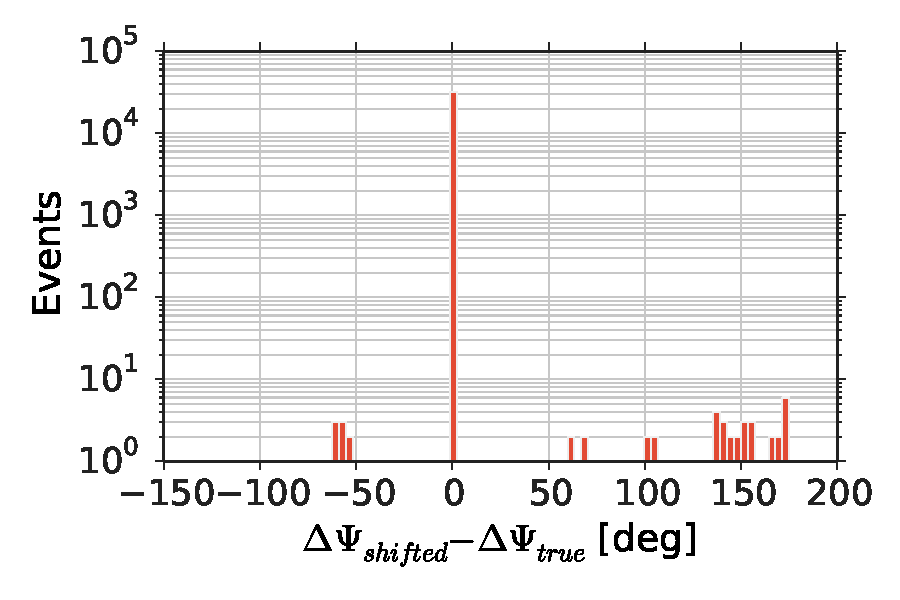
\includegraphics[width=
1.\textwidth]{fig/shift2source_true_minus_shifted_error.pdf}
  \caption{\label{fig:shift2source_proof}Shown is the difference between the
true error between reconstructed and true direction and the error between the
shifted reconstructed direction and the GRB direction. Almost all events have 
been shifted perfectly.}
\end{figure}

\begin{figure}[h]
\centering
 \captionsetup{width=.9\textwidth}
%  \captionsetup{margin=0pt}
\subfloat[Dependency on zenith angle.\label{fig:shift2source_zendependency}]{%
 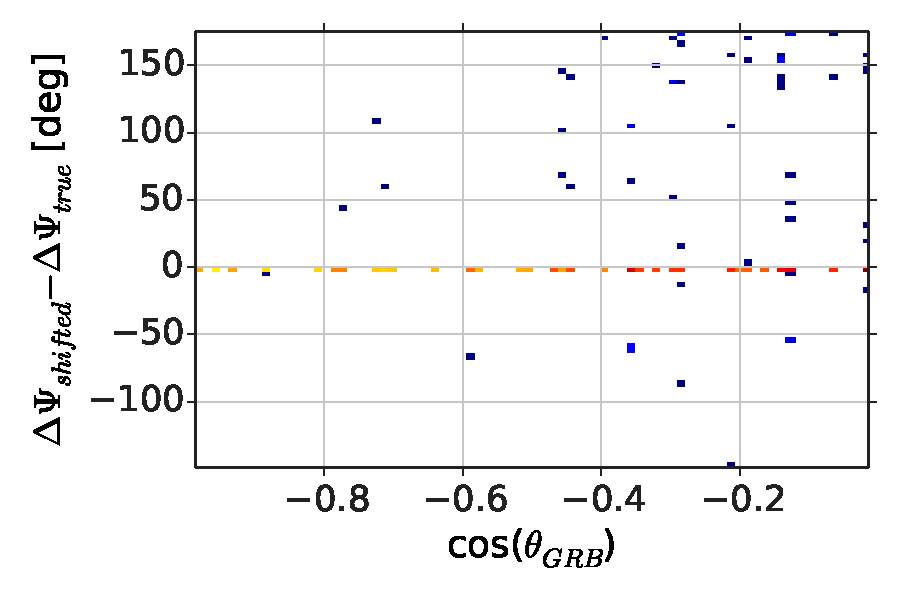
\includegraphics[width=0.45\textwidth]{fig/shift2source_zendependency.pdf}}
 \subfloat[Dependency on the azimuth angle. 
\label{fig:shift2source_azidependency}]{%
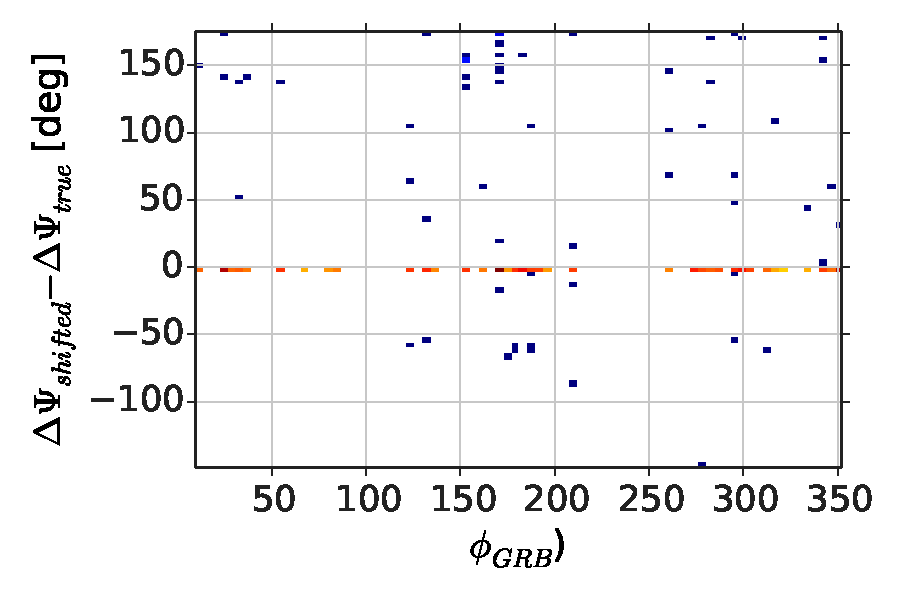
\includegraphics[width=0.45\textwidth]{fig/shift2source_azidependency.pdf}}
\caption{Two dimensional histograms showing the dependency of the difference 
between shifted and true reconstruction error to the zenith (left) and azimuth 
angle (right). No true dependency can be seen.}
\end{figure}

Figure \ref{fig:shift2source_proof} demonstrates that, for almost all events, 
the new directions 
have
 the same distance to the GRB as the originally
reconstructed directions had compared to their true directions. There are few 
events \textbf{(I need a percentage here!!!???)} for which the process doesn't 
work. The reasons are unknown at this point. Figures 
\ref{fig:shift2source_zendependency} and \ref{fig:shift2source_azidependency} 
demonstrate that there is no directional correlation. However, as this effect 
is only true for ???\% of the events, the effect can be neglected.
% An example skymap for one GRB and the correspondingly shifted neutrino
% directions is shown in Figure \ref{fig:skymap_grb}.




\subsubsection{Total Emitted Energy as Source $\hat{E}_{\nu, \text{total}}$}
\label{sec:Etotal}
So far, the steps dealing with simulation effects and neutrino directions have
been described. To calculate $N_\text{exp}^\nu$ the differential particle
fluence in energy at earth needs to be calculated as well, based on parameters
that are drawn as part of the simulation (chapter \ref{sec:drawnProp}). A first
step is to calculate the total emitted energy in neutrinos at the source
$\hat{E}_{\nu, \text{total}}$.

The peak luminosity and the 90\% time window can be used if the light curve is
known. In
this work a fast rise and rapid decay (FRED) light curve with an instant jump
to the peak luminosity and an exponential decay afterwards is assumed. 

%comment about test if this is folded into normalization?

The luminosity at a given time $\hat{t}$ is defined as 
\begin{equation}
 \hat{L}(\hat{t}) = \hat{L}_{\text{Peak}} \cdot e^{\left(-
\frac{\hat{t}}{\hat{\tau}}\right)}
\label{eq:lum_vs_time}
\end{equation}
The total energy is the time integral over the time dependent luminosity
distribution
\begin{equation}
\label{eq:Eiso}
\begin{align}
 \hat{E}_{\nu, \text{total}} & =  \int_0^{\infty} \hat{L}(\hat{t}) d\hat{t} 
	  =  \hat{L}_{\text{Peak}} \int_0^{\infty} e^{-\frac{t}{\tau}} dt\\
	 & = - \hat{\tau} \cdot \hat{L}_{\text{Peak}} \left[
e^{-\frac{\hat{t}}{\hat{\tau}}}
\right]_0^{\infty}
          = \hat{\tau} \cdot \hat{L}_{\text{Peak}}
\end{align}
\end{equation}
The final shape of the distribution depends on the unknown $\tau$ which needs to
be replaced by a known quantity such as the 90 \% time window
$\hat{t}_{90}$ in which 90\% or $\hat{E}_{\nu, 90}=0.9 \cdot \hat{E}_{\nu,
\text{total}}$ are
observed. 
The amount of energy radiated within this time can be determined with
\begin{equation}
 \begin{align}
  \hat{E}_{\nu, 90} & = 0.9 \cdot \hat{E}_{\nu, \text{total}} = 0.9 \cdot
\hat{\tau} \hat{L}_{\text{Peak}} = 
\int_0^{\hat{t}_{90}} \hat{L}(\hat{t}) d\hat{t} \\
         & = - \hat{\tau} \hat{L}_{\text{Peak}}
\left[e^{-\frac{\hat{t}}{\hat{\tau}}} \right]_0^{\hat{t}_{90}}
= \hat{\tau} \hat{L}_{\text{Peak}} \left[1 -
e^{-\frac{\hat{t}_{90}}{\hat{\tau}}} \right]
 \end{align}
\end{equation}
leading to 
\begin{equation}
 \begin{align}
  \left[ 1 - e^{-\frac{\hat{t}_{90}}{\hat{\tau}}} \right] &= 0.9 \\
 0.1 & = e^{-\frac{\hat{t}_{90}}{\hat{\tau}}} \\
 \text{ln}(0.1) & = -\frac{\hat{t}_{90}}{\hat{\tau}}\\
 \Rightarrow \hat{\tau} &= \frac{-\hat{t}_{90}}{\text{ln}(0.1)}
 \label{eq:ToyMC_tau}
 \end{align}
\end{equation}
Entering this in equation \ref{eq:Eiso} leads to:
\begin{equation}
 \hat{E}_{\nu, \text{total}} = - \hat{L}_{\text{Peak}}
\frac{\hat{t}_{90}}{\text{ln}(0.1)}
\end{equation}


\subsubsection{Fluence at Source}
The simulation draws GRB properties at source. In the first step they are used
to calculate the differential particle fluence in energy
$\frac{d\hat{F}_P}{d\hat{E}}$ in units $\text{GeV}^{-1}
\text{s}^{-1}\text{sr}^{-1} \text{cm}^{-2}$ at a small co-moving distance from
the source $\hat{d}_0$. The spectral shape is a generalization based on the fits
to the HESE flux (eq. \ref{eq:HESEflux_gen}).

\begin{equation}
 \frac{d\hat{F}_P}{d\hat{E}} = \frac{\hat{F}_0}{4 \pi \hat{d}_0^2} \cdot
\hat{E}^{-\gamma} \text{exp} \left( - \frac{\hat{E}}{\hat{E}_\text{cut}} \right)
\end{equation}
The fluence normalization $\hat{F}_0$ is unknown. However, in the previous
section \ref{sec:Etotal} the total emitted energy was calculated. It equals the
integral over $\hat{E} \cdot \frac{d\hat{F}_P}{d\hat{E}}$.

\begin{equation}
\label{eq:Etotal}
 \hat{E}_{\nu, \text{total}} = \int_{\hat{E}_{min}}^\infty \hat{E} \hat{F}_0
\hat{E}^{-\gamma} \text{exp} \left(  -
\frac{\hat{E}}{\hat{E}_\text{cut}}\right) d\hat{E} = \hat{F}_0
\Upsilon \left(\hat{E}_{min}, \hat{E}_\text{cut}\right)
\end{equation}
The result depends on two GRB parameters which are chosen equally as physics 
parameters
for all GRBs: A minimal energy of the neutrinos $\hat{E}_{min}$ and the
break energy $\hat{E}_{cut}$. Once, these parameters are chosen, $\Upsilon$ is
a constant for all GRBs and the differential particle fluence in energy at
source can be written as

\begin{equation}
 \frac{d\hat{F}_P}{d\hat{E}} = \frac{\hat{E}_{\nu, \text{total}}}{4 \pi
d_0^2\Upsilon\left(\hat{E}_{min}, \hat{E}_\text{cut}\right)} \cdot
\hat{E}^{-\gamma}
\text{exp} \left( - \frac{\hat{E}}{\hat{E}_\text{cut}} \right)
\label{eq:partFluenceS}
\end{equation}
%  The impact 

\subsubsection{Fluence at Earth}
\label{sec:FatEarth}
Having derived the fluence at source, cosmological effects need to be taken
into account when calculating the fluence at earth. The energy and time
at source relate to the values at earth with $\hat{E} = (1 + z) E$ and 
$\hat{t} = \frac{t}{1+z}$. 
The energy flux at earth $\Phi_E$ is linked to the luminosity via
\begin{equation}
\label{eq:PhiEL}
 \Phi_E (t) = \frac{\hat{L} \left(\hat{E}, \hat{t} \right)}{4 \pi d_l^2} =
\frac{L \left(E, t \right)}{4 \pi d_l^2}
\end{equation}
with the luminosity distance $d_l=(1+z) \cdot d_c$.
The particle fluence $F_P$ at earth is the time integrated particle flux
$\Phi_P$ which in turn is the energy derivative of the energy flux.
\begin{equation}
F_P(E) = \int \Phi_P(E,t)\, dt = \int
\frac{d\Phi_E(E,t)}{dE}\,dt 
% = \frac{dN(E)}{dA}
\label{eqn:fluence}
\end{equation}

% \begin{equation}
% \Phi_E (t) = \int \Phi_P(E,t) \, dE = \int \frac {dN(E,t)}{dA\,dt}\, dE.
% \label{eqn:fluxes}
% \end{equation}
% \begin{eqnarray}
%   \frac {dN(E,t)}{dA\,dt} = \Phi_P =  \frac{d\Phi_E(E,t)}{dE}
%    & = & \frac{1}{4 \pi d_l^2} \frac {d L(t)}{dE}
% \end{eqnarray}
% \begin{eqnarray}
% \frac {dF_P(E)}{dE} = \frac {dN(E)}{dA\,dE} & = &  \int \frac{\Phi_P(E,t)}{dE}\,
% dt %\\
% %   & = & \frac{1}{4 \pi d_l^2} \int \frac{d^2 L(t)}{dE^2} dt
%   \label{eqn:local}
% \end{eqnarray}
The energy flux can be replaced with the luminosity according to
\ref{eq:PhiEL}. Applying a derivation in energy and transforming energy and
time to the source frame, one obtains
\begin{eqnarray}
  \frac {dF_P(E)}{dE}
     & = &  \frac{1}{4 \pi d_l^2} \int \frac{d^2 L(t)}{dE^2} dt \\
     & = &  \frac{1}{4 \pi d_l^2} \int \frac{d^2 L(\hat{t})}{d\hat{E}^2}
     \frac{d^2\hat{E}}{dE^2} \frac{dt}{d\hat{t}}
     d\hat{t} \\
     & = & \frac{(1+z)^3} {4 \pi d_l^2} \int \frac{d^2 L(\hat{t})}{d\hat{E}^2}
     d\hat{t}
     \label{eqn:final}
\end{eqnarray}
A similar equation is true for differential particle fluence in energy near the
source at a distance $d_0$.
\begin{eqnarray}
\frac {d\hat{F}_P(\hat{E})}{d\hat{E}}
  & = & \frac{1}{4 \pi d_0^2} \int \frac{d^2 L(\hat{t})}{d\hat{E}^2} d\hat{t}
  \label{eqn:grb}
\end{eqnarray}
Combining equation \ref{eqn:final} and \ref{eqn:grb} relates the differential
particle fluence at earth to the differential particle fluence at source
derived in \ref{eq:partFluenceS}.
\begin{eqnarray}
  \frac{dF_P(E)}{dE}
    & = & \left(\frac{d_0}{d_l}\right)^2 (1+z)^3 \frac
{d\hat{F}_P(\hat{E})}{d\hat{E}} \\
&=& \frac{\hat{E}_{\nu, \text{total}}}{4 \pi
d_l^2\Upsilon\left(\hat{E}_{min}, \hat{E}_\text{cut}\right)} \cdot
\hat{E}^{-\gamma}
\text{exp} \left( - \frac{\hat{E}}{\hat{E}_\text{cut}} \right) \cdot (1+z)^3 \\
&=& \frac{\hat{E}_{\nu, \text{total}}}{4 \pi
d_l^2\Upsilon\left(\hat{E}_{min}, \hat{E}_\text{cut}\right)} \cdot
E^{-\gamma}
\text{exp} \left( - \frac{E \cdot (1+z)}{\hat{E}_\text{cut}} \right) \cdot
(1+z)^{3 - \gamma}
\end{eqnarray}
In the last step the energy at source was replaced with the energy at earth in
consideration of the cosmological effects. This formula can now be used to
calculate the number of expected neutrinos within IceCube given the drawn
properties and a nugen dataset (section \ref{subsubsec:NExp}).

\subsubsection{Number of Expected Neutrinos Within IceCube}
\label{subsubsec:NExp}
This chapter described how the differential particle fluence in energy can be
derived from the drawn parameters describing a GRB in this simulation. The
number of expected neutrinos is  given with

%??? detail about  nugen and oneweight. cite paper on oneweight. detector
% response

\begin{equation}
\begin{align}
 N_\text{exp}^\nu & = \sum_i\frac{dF_P(E_i)}{dE} \cdot
\frac{OneWeight_i}{N_\text{generated} \cdot A_{ZB}} \\
&= \sum_i \cdot \frac{\hat{E}_{\nu, \text{total}}}{4 \pi
d_l^2\Upsilon\left(\hat{E}_{min}, \hat{E}_\text{cut}\right)} \cdot
E_i^{-\gamma}
\text{exp} \left( - \frac{E_i \cdot (1+z)}{\hat{E}_\text{cut}} \right) \cdot
(1+z)^{3 - \gamma}
\frac{OneWeight_i}{N_\text{generated} \cdot \frac{A_{ZB}}{4 \pi}}
\end{align}
\end{equation}
It is dependent on various factors of the nugen simulation and some parameters
from the derivation of the differential particle fluence. The nugen simulation
describes the probability for each simulated event $i$ to reach the detector,
interact within its effective volume and to be detected ($OneWeight_i$), the
individual energy $E_i$, the number of generated MC neutrino events
$N_\text{generated}$ and a re-weighting factor $\frac{A_{ZB}}{4 \pi}$. The
re-weighting factor has been explained in more detail in section ???. 

Furthermore, the number of expected neutrinos is dependent on the redshift of
the GRB, the total emitted energy in neutrinos $\hat{E}_{\nu, \text{total}}$ -
and thus $\hat{L}_\text{Peak}$ and $\hat{t}_{90}$ - as well as the constant
$\Upsilon$. The constant itself is dependent on the energy of the cut-off
$\hat{E}_\text{cut}$ and the minimal neutrino energy at source $\hat{E}_{min}$.
As described in ??? the cut-off energy will be optimized to reproduce the
observed cut-off or set to very high values depending on the spectrum that is
used (see ???). The effect of the minimal energy can be either absorbed into
the normalization to the HESE flux (chapter \ref{sec:norm2HESE}) or specific
cases and their impact can be studied (chapter ???).
\subsection{Normalization to HESE Flux}
\label{sec:norm2HESE}
% \begin{itemize}
%  \item my way: average Lpeak, average t90, integrate over ???
%  \item same result.
%  \item table of results??? once I have final dataset?
%  \item plot
%  \item influence of emin: upsilon but also not considering events with
% E<E(1+z)???
% \end{itemize}
The luminosity is drawn according to the luminosity function fitted to
gamma-ray data, assuming the neutrino luminosity function to follow the
same shape. However, a normalization factor might be needed to trim it to the
correct energies and consequently to the correct number of neutrinos to produce
the HESE flux. ($N_\text{exp}^\nu \propto \hat{E}_{\nu, \text{total}} \propto
L_\text{Peak}$). Equation \ref{eq:Nexp_wZB} evolves to
% \begin{equation}
% \label{eq:Nexp_wZB_wEps}
%  N_\text{exp}^\nu = \sum_i\frac{dF_P(E_i)}{dE_i} \cdot
% \frac{OneWeight_i}{N_\text{generated}}
% \end{equation}
\begin{eqnarray}
\label{eqn:Nexp_wZB_wEps}
 N_\text{exp}^\nu &= & \epsilon \cdot \sum_i \cdot \frac{\hat{E}_{\nu,
\text{total}}}{4 \pi
d_l^2\Upsilon\left(\hat{E}_{min}, \hat{E}_\text{cut}\right)} \cdot
E_i^{-\gamma}
\text{exp} \left( - \frac{E_i \cdot (1+z)}{\hat{E}_\text{cut}} \right) \cdot
(1+z)^{3 - \gamma}
\frac{OneWeight_i}{N_\text{generated} \cdot \frac{A_{ZB}}{4 \pi}} \\
&= & \epsilon^* \cdot \sum_i \cdot \frac{\hat{E}_{\nu, \text{total}}}{4 \pi
d_l^2} \cdot
E_i^{-\gamma}
\text{exp} \left( - \frac{E_i \cdot (1+z)}{\hat{E}_\text{cut}} \right) \cdot
(1+z)^{3 - \gamma}
\frac{OneWeight_i}{N_\text{generated} \cdot \frac{A_{ZB}}{4 \pi}}
\label{eqn:Nexp_wZB_wEpsStar}
\end{eqnarray}
Once $\hat{E}_{min}$ (chapter ???) and $\hat{E}_\text{cut}$ are determined,
$\Upsilon$ is a constant for every GRB which can be included in an effective
normalization factor
\begin{equation}
\epsilon^* =
\frac{\epsilon}{\Upsilon\left(\hat{E}_{min}, \, \hat{E}_\text{cut}\right)}
\end{equation}
Due to the effective normalization factor it is redundant to calculate the
constant $\Upsilon$. However, a different $\epsilon^*$ needs to be determined
for different $\hat{E}_{min}$. The impact of choosing different minimal
energies is studied in chapter ???.

There are two ways to determine $\epsilon$ - a Monte Carlo based and a semi
analytic one.
\subsubsection{$\epsilon^*$ - Monte Carlo Based}
This approach was followed by Nora Strotjohann. Given the different
spectra fitted to the HESE flux (chapter \ref{sec:GRBSpectra}), a different
number of neutrinos per year are expected due to GRBs. Using the nugen
simulation without the GRB simulation one can simply calculate the number of
neutrinos using the spectra fitted at earth. They are displayed in figure
\ref{fig:Espectra}. Their shape is quite similar at high energies at which the
HESE events were found. However, the curves diverge quite significantly at
lower energies leading to different predictions about the number of neutrinos
one could expect from GRBs on OFU level.

\begin{figure}[h]
\centering
 \captionsetup{width=.68\textwidth}
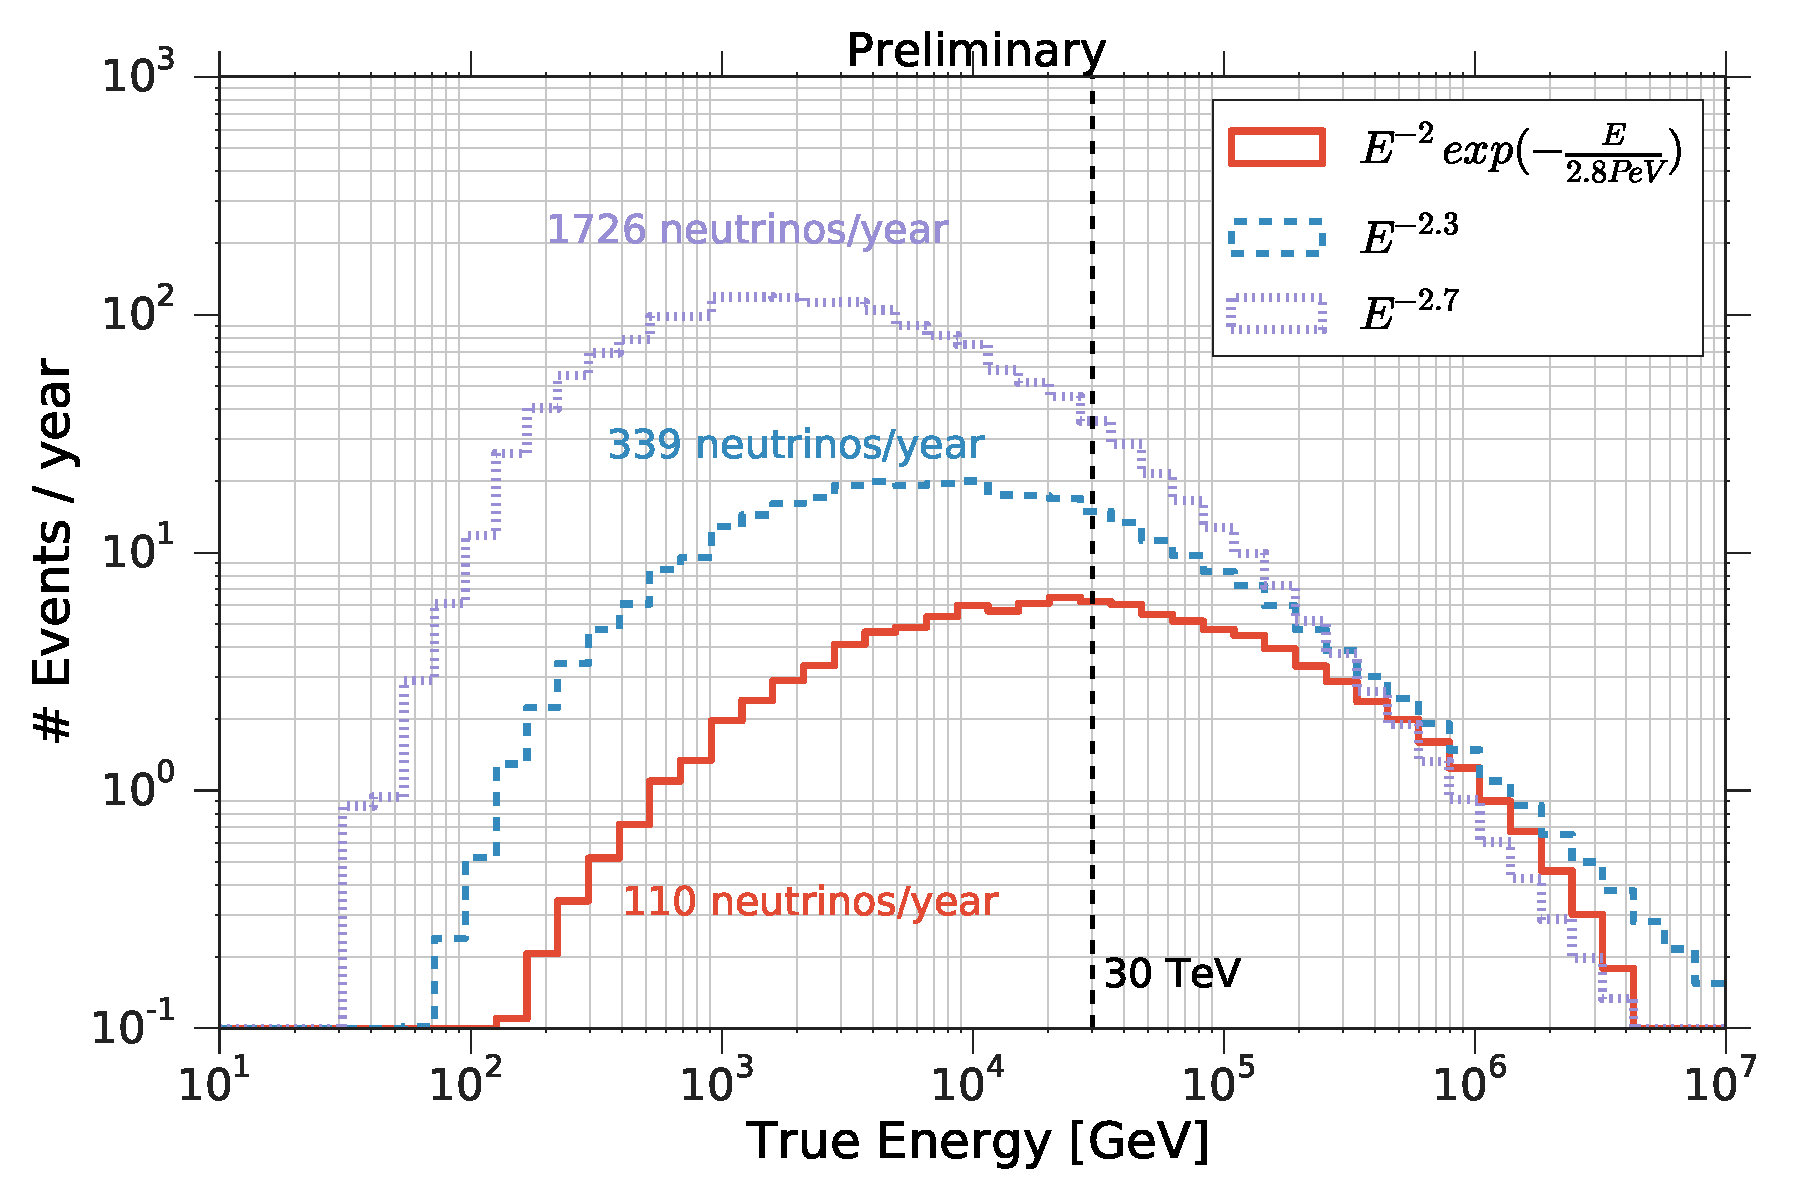
\includegraphics[width=0.68\textwidth]{fig/Spectra_on_OFU.pdf}
    \caption{The three different spectra fitted to the HESE events on OFU
level. The true neutrino energy is used. The number of expected neutrinos is
highly dependent on the chosen spectrum.}
\label{fig:Espectra}
\end{figure}

To determine $\epsilon^*$ up to 5 million GRBs ($N_\text{GRB, sim}$) are
simulated with $\epsilon^*$ set to one. The sum over $N_\text{exp}^\nu$ of all
GRBs is renormalized to the number of expected GRBs per year
$N_\text{GRB, yr}$ and needs to reproduce the number of expected neutrinos on
OFU level.
\begin{equation}
\epsilon^*  = \frac{N_\text{exp}^\nu (\epsilon^* = 1) \cdot
\frac{N_\text{GRB, yr}}{N_\text{GRB, sim}}}{N_{\text{exp, OFU}}^\nu}
\end{equation}
The final result depends on the number of expected GRBs per year which is an
uncertain number. Fortunately, it is a linear factor and $\epsilon^*$ can be
changed easily with the knowledge with which $N_\text{GRB, yr}$ it was
calculated.
\begin{equation}
 \epsilon_\text{new}^* = \epsilon^* \cdot \frac{N_\text{GRB,
yr}^\text{new}}{N_\text{GRB,yr}}
\end{equation}



\subsubsection{$\epsilon^*$ - Semi-Analytic Approach}
The second approach integrates over the expected differential fluxes in energy
from all GRBs up to the maximal chosen redshift ($z_{max}=8$) under
consideration of their redshift distribution.
\begin{eqnarray}
 \Phi_\text{GRB} &=& \int_{z=0}^{z=8} dz \, R(z) \cdot \frac{dF_P \left(z,  E,
\hat{E}_{\nu, \text{total}} \left(\hat{t}_{90}, \, L_\text{Peak}\right)
\right)}{dE} \\
&=& \int_{z=0}^{z=8} dz \, R(z) \cdot \frac{\hat{E}_{\nu, \text{total}}}{4 \pi
d_l^2(z)} \cdot
E_i^{-\gamma}
\text{exp} \left( - \frac{E_i \cdot (1+z)}{\hat{E}_\text{cut}} \right) \cdot
(1+z)^{3 - \gamma}
\end{eqnarray}
The final result needs to equal the measured fluxes on earth over the  whole
energy range and the flux is recalculated for 100 energy values between $10$
and $10^9$ GeV evenly spaced in $\text{log} E$.

Next to the redshift of the GRBs and the energy of the neutrinos the signal
expectation is dependent on the
total energy in neutrinos and thus the peak luminosity and the $\hat{t}_{90}$
values. The average value is calculated based on an average time window and
peak luminosity. The average time window $<\hat{t}_{90}>$ was determined out of
5 million drawn values while the average peak luminosity is calculated
according to
\begin{equation}
\begin{align}
 <L_\text{Peak}> &=
\frac{\int_{L_\text{Peak}^{min}}^{L_\text{Peak}^{max}} L_\text{Peak}
\cdot \Phi(L_\text{Peak})
d\text{log}_{10}L_\text{Peak}}{\int_{L_\text{Peak}^{min}}^{L_\text{Peak}^{max}
}\Phi(L_\text{ Peak})
d\text{log}_{10}L_\text{Peak}}\\
&= \frac{\int_{L_\text{Peak}^{min}}^{L_\text{Peak}^{max}} L_\text{Peak}
\cdot
\frac{\Phi(L_\text{Peak})}{L_\text{Peak} \text{ ln}(10)}
dL_\text{Peak}}{\int_{L_\text{Peak}^{min}}^{L_\text{Peak}^{max}}\frac{
\Phi(L_\text{ Peak})}{L_\text{Peak}
\text{ ln}(10)} dL_\text{Peak}}\\
&=
\frac{\int_{L_\text{Peak}^{min}}^{L_\text{Peak}^{max}}\frac{\Phi(L_\text{
Peak})}{\text{ln} (10)}
dL_\text{Peak}}{\int_{L_\text{Peak}^{min}}^{L_\text{Peak}^{max}}\frac{
\Phi(L_\text{ Peak})}{L_\text{Peak}
\text{ ln}(10)} dL_\text{Peak}}
\end{align}
\end{equation}

%table with average values ???


The co-moving rate density $R(z)$ includes a normalization to the number of
expected GRBs according to said model. If a different number of GRBs is
assumed, then the resulting flux needs to be adjusted by an according factor.

This flux of all GRBs up to a redshift of eight needs to reproduce the HESE
flux over the whole energy range (Fig. \ref{fig:Phi_norm}). This can be
achieved for the two spectra without a cut-off.
However, the HESE flux can not be reproduced at very high energies using the
same
exponential cut-off for all GRBs at all redshifts. $\hat{E}_\text{cut}$ was
chosen such that an exact agreement was reached for the most part of the energy
range accepting a disagreement in the tail. Possibly, one could determine an
energy dependent $\epsilon^*$. However, given the few numbers of events at
these energies and the lack of knowledge of the exact shape of the cut-off due
to missing HESE statistic this extra complication was not attempted.
\begin{equation}
 \epsilon^* = \frac{\Phi_\text{HESE}(E)}{\Phi_\text{GRB}(E)}
\end{equation}
The effective efficiency factor can be applied in the further simulation to
each GRB using equation \ref{eqn:Nexp_wZB_wEpsStar}.

Both methods of determining $\epsilon^*$ agree in the order of 1\%. The 
disagreement could result from a random extra bright GRB in the sample used in 
the Monte Carlo based method and / or the calculation precision set for the 
semi-analytic approach.
\begin{figure}[h]
 \centering
 \captionsetup{width=.9\textwidth}
\subfloat[$\hat{E}_{min}$ was set to 1.\label{fig:Phi_norm}]{%
 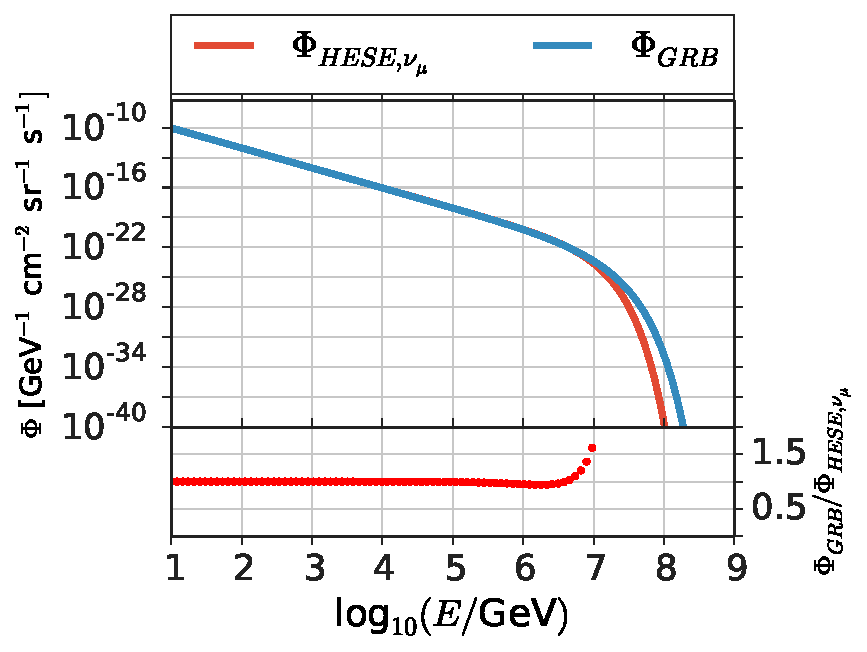
\includegraphics[width=0.45\textwidth]{fig/Phi_norm_gamm2.pdf}}
\subfloat[$\hat{E}_{min}$ was set to $10$ 
TeV.\label{fig:Phi_norm_Emin}]{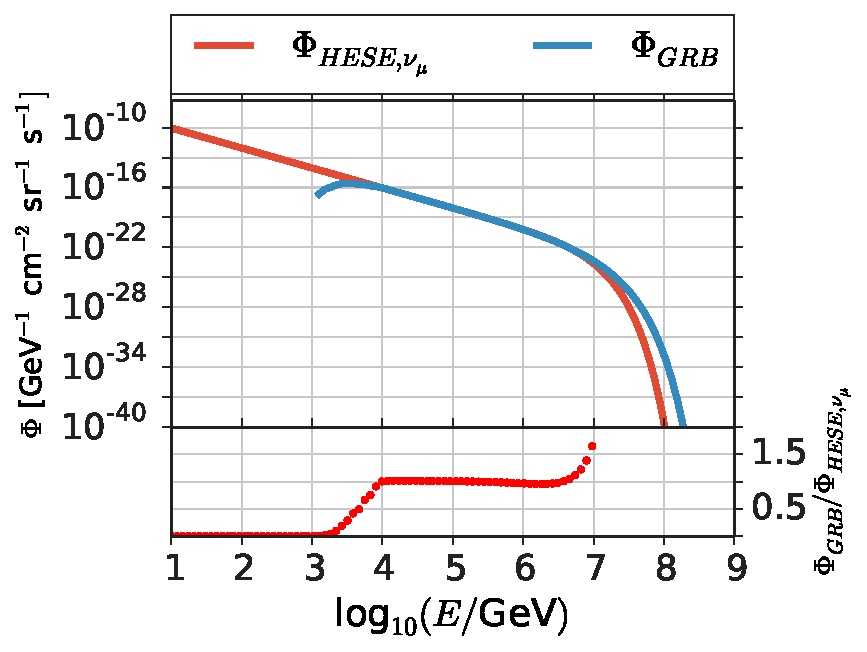
\includegraphics[width=0.45\textwidth]{%
fig/Phi_norm_gamm2_Emin.pdf}}
 \caption{Upper plot: The differential flux in energy for the HESE spectrum
($E^{-2}$ with cut-off) and the spectrum produced by all GRBs up to a redshift
of 8. \\
Lower plot: ratio between the GRB flux and the HESE flux. The ratio should be
queal to one.}
\end{figure}
% emin plot with Emin=10000???



\subsubsection{Influence of $\hat{E}_{min}$}
The influence of the minimal neutrino energy from a GRB has two effects.

The constant $\Upsilon$ in eq. \ref{eqn:Nexp_wZB_wEps} becomes smaller the more
stringent the energy cut is (Eq. \ref{eq:Etotal}) leading to a smaller
efficiency factor $\epsilon$ as the flux at each energy needs to
reproduce the HESE flux. The effective efficiency factor $\epsilon^*$ will stay
the same.
Using the example of $\hat{E}_{min} = 10 \text{ TeV}$ shown in figure
\ref{fig:Phi_norm_Emin}, $\epsilon^*$ was chosen such that an agreement was
found for as large an energy range as possible. Considering all energies (Fig.
\ref{fig:Phi_norm}) $\epsilon^*=0.149$ was determined while applying a minimal
energy leads to  $\epsilon^*=0.151$. The discrepancy of about 1.5 \%  is
probably due to the precision of agreement between the two fluxes required in
the procedure. \textbf{can i do better? I think that I did. checkout 
$emin_redon.ipynb$}

The other effect can be seen at low energies at which the GRB flux drops to
zero. No events with energies
\begin{equation}
 E_\nu \leq \frac{\hat{E}_{min}}{1+z}
\end{equation}
can exist in the detector if a minimal neutrino energy cut at source is
applied. The GRB flux transitions from an agreement with the HESE flux towards
no flux at all because the cut effects are redshift dependent. Neutrinos 
with higher
energies are more effected the  closer to earth a GRB is assumed to be.

In summary, the effect of a different $\hat{E}_{min}$ on the final flux per
energy is non existent. However, events will be lost at lower energies. 

%result table ???


\subsection{Detection Probabilities}
At this stage, the drawing of GRB properties according to the specified 
functions
and the subsequent derivation and calculation of the signal expectation in
IceCube has been explained. However, the Optical (and X-ray) Follow-Up does not
trigger on singlets but on multiplets fulfilling several criteria.

Multiplets are a number of neutrinos that arrive within 100 s and 3.5 degrees
of each other (chapter \ref{sec:OFU_alert_system}). A test statistic was 
implemented to select the
most signal like doublets to trigger Swift Follow-Up observations. Once 
triggered there
is a chance that a source will not be within the FoV of the XRT. The 
probabilities for two neutrinos to pass these criteria will be 
explained in this section.

\subsubsection{Doublet Probabilities}

\paragraph{Probability to detect two neutrinos $P_{2 \nu}$}$\;$\\
In section \ref{subsubsec:NExp}, the number of expected neutrinos per 
GRB $\mu$ was calculated. 
Given this number, the probability to see $N$ neutrinos is given with the 
Poisson 
distribution
\begin{equation}
  P_\text{Poisson}(N, \mu) = \frac{\mu^N}{N!} \exp^{-\mu}
\end{equation}
Hence, the probability to see exactly one neutrino and one or more neutrinos is 
\begin{eqnarray}
 P_{1 \nu} &= P_\text{Poisson}(1, \mu) \\
 P_{\geq 1 \nu} &= 1 - P_\text{Poisson}(0, \mu)
\end{eqnarray}
The subsequent probabilities apply to the case of exactly two detected 
neutrinos.
\begin{equation}
 P_{2\nu} = P_\text{Poisson}(2, \mu) = \frac{\mu^2}{2!} \exp^{-\mu}
\end{equation}


\paragraph{P$_{\Delta t}$}$\;$\\
% \\
%  \Rightarrow \tau &= \frac{-t_{90}}{\text{ln}(0.1)}
P$_{\Delta t}$ is the probability that two neutrinos arrive within
100 seconds, the time window
specified in the doublet search. 
It decreases exponentially with time if the lightcurve is assumed to be fast 
rising
with an exponential decay (FRED)
\begin{equation}
 P(\Delta t) = 1 - e^{\left(-\frac{\Delta t}{\tau} \right)}.
\end{equation}
$\tau$ can be determined according to equation \ref{eq:ToyMC_tau} given
a specific $t_{90}$ (drawn according to \ref{eq:t90dist} and converted in 
agreement
with \ref{eq:t90earth}). For the Optical Follow-Up
$\Delta t_{max} =100 \text{ s}$ is currently set. 
%more detail here? too much just refering to other equations?
The effects of different time
windows could be examined by choosing different values. However, this is not
the focus of this work.



\paragraph{P$_{3.5^\circ}$}$\;$\\
The second requirement for each neutrino pair is that they arrive with a
maximum angular separation of 3.5 degrees. To calculate this probability 
P$_{3.5^\circ}$ for a given GRB, NuGen events need to be
selected from within the zenith band (chapter \ref{sec:zenith_bands}) and
shifted to the GRB direction (chapter \ref{sec:shift2source}). 
% Each remaining event is paired with all other events, 
To save on computation time, 4000 of the NuGen events are selected randomly
and the angular 
differences of the
shifted reconstructed directions are determined for each event combination. The 
probability is then the
ratio between the sum of the weight products (term $i$ and $j$ in Eq. 
\ref{eqn:Nexp_wZB_wEps}) of
all event pairs passing the $3.5^\circ$ cut and all evaluated pairs
\begin{equation}
\label{eq:P3p5}
 P_{3.5^\circ} = \frac{\sum_{i} \sum_{j=i+1} w_i \cdot w_j | \Delta \Psi(i, j)
\leq
3.5^{\circ}}{\sum_i \sum_{j=i+1} w_i \cdot w_j}
\end{equation}
Though selecting 4000 events randomly speeds up this calculation, combining 
each event of the selection with all others requires computational power 
and time. 
If all events from within the zenith bands were to be considered, all events 
and therefore the probability $P_{3.5^\circ}$ should be the same for all GRBs 
coming from the exact same zenith angle suggesting that a parameterization in 
dependence of the drawn GRB zenith angle should be possible. 

About 8000 GRBs are drawn for each season and HESE spectra
%  and GRB model 
and the probability calculated according to \ref{eq:P3p5}. The resulting 
parameterization 
$P_{3.5^\circ}(\theta_\text{GRB})$ is then used to simulate GRBs in greater 
numbers.
Exemplary, two cases are shown here to demonstrate the quality and the 
different behavior of the parameterization in different seasons.

The probabilities follow different behaviors in different zenith ranges. Using 
a 
hard spectrum with $\gamma=2$ and the NuGen dataset of the BDT season, the 
probability is displayed  vs
$\theta_\text{GRB}$ in a 2d histogram in Fig. \ref{fig:P3p5param_bdt_gamma2}. A 
mean probability value is calculated for each $\theta_\text{GRB}$ bin.
The probability follows two different functional behaviors. A hyperbolic 
tangent is fitted to the data near the pole ($\cos(\theta_\text{GRB}) 
\leq -0.81$)
\begin{equation}
\label{eq:Ptanh}
 P = a \cdot \text{tanh}(b \cdot (\cos(\theta_\text{GRB}- c)) + d
\end{equation}
while a simple polynomial function of the fifth order is used in the second 
region
\begin{equation}
\label{eq:PPoly}
 P = a \cdot \cos^5\theta_\text{GRB} + b \cdot 
\cos^4\theta_\text{GRB} + c \cdot \cos^3\theta_\text{GRB} + d 
\cdot \cos^2\theta_\text{GRB} + e \cdot \cos\theta_\text{GRB} + f
\end{equation}
Next to the mean probability of each bin, the fits use the coordinates of 
the mean of these averaged values between the 
last bin of the first region and the first bin of the last region and the 
splitting zenith value as an additional data point.
The quality of the parameterization was examined by creating a second dataset 
of GRBs. The probability was calculated according to Eq. 
\ref{eq:P3p5} based on all 
NuGen events within a zenith region around a GRB ($P_{3.5^\circ}^\text{MC}$) 
and parametrized according to the fit to the first 
dataset ($P_{3.5^\circ}^\text{param}$).
% to characterize the probability with the most 
% information available.
A good agreement between the two procedures is presented in Fig. 
\ref{fig:P3p5param_bdt_gamma2_quality} with a maximum deviation of about 1\%.

\begin{figure}[h]
\centering
 \captionsetup{width=.9\textwidth}
\subfloat[Parametrization (blue line) of the 
probability $P_{3.5^\circ}$\label{fig:P3p5param_bdt_gamma2}]{%
  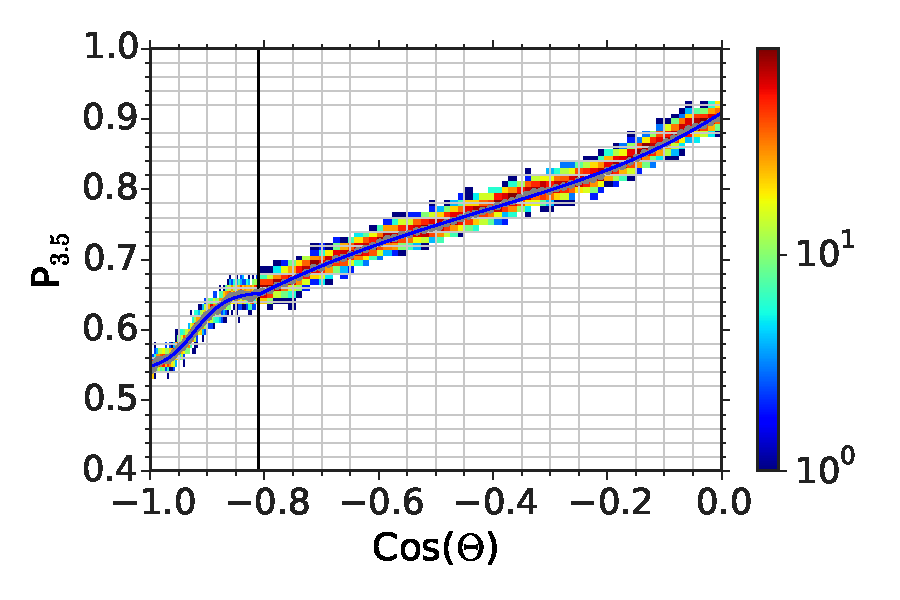
\includegraphics[width=0.45\textwidth]{fig/P3p5param_bdt_gamma2.pdf}}
\subfloat[Testing the 
parameterization with a second 
dataset.\label{fig:P3p5param_bdt_gamma2_quality}]{%
  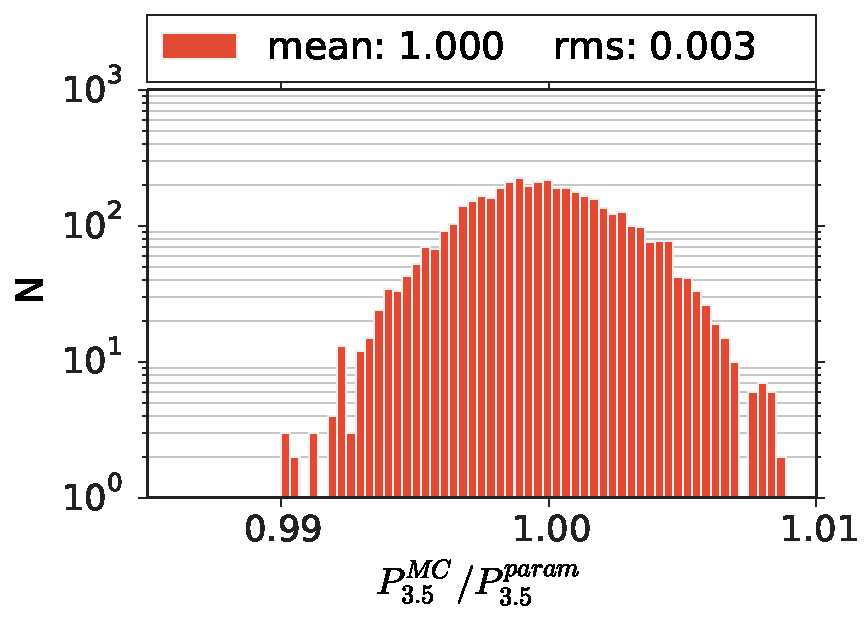
\includegraphics[width=0.45\textwidth]{fig/P3p5param_bdt_gamma2_quality.pdf}}
\caption{IC86-BDT season: The probability of neutrino events to be within 3.5\% 
of each other and the dependency on the cosinus of the GRB zenith angle. The 
blue line represents the parameterization (left). Using a second set of 
simulated GRBs, a histogram 
of the ratio between the calculated probabilities based on all events in 
the zenith bands and the parametrized values is shown (right). The maximum 
deviation 
is about 1\%.}
\end{figure}

The second example (IC86-2) demonstrates the difference between the IC86-1/2 
seasons 
and the BDT season. The dependence of the zenith angle shows more structure 
(Fig \ref{fig:P3p5param_862_gamma2}) and the parameterization is split into 
four regions. The data in the first one starting at the pole is fitted with a
hyperbolic tangent (Eq. \ref{eq:Ptanh}) while the data in the other three 
regions are all fitted with the polynomial function (Eq. \ref{eq:PPoly}) each.

\begin{figure}[h]
\centering
 \captionsetup{width=.9\textwidth}
%  \captionsetup{margin=0pt}
 \subfloat[Parametrization (blue line) of the 
probability $P_{3.5^\circ}$\label{fig:P3p5param_862_gamma2}]{%
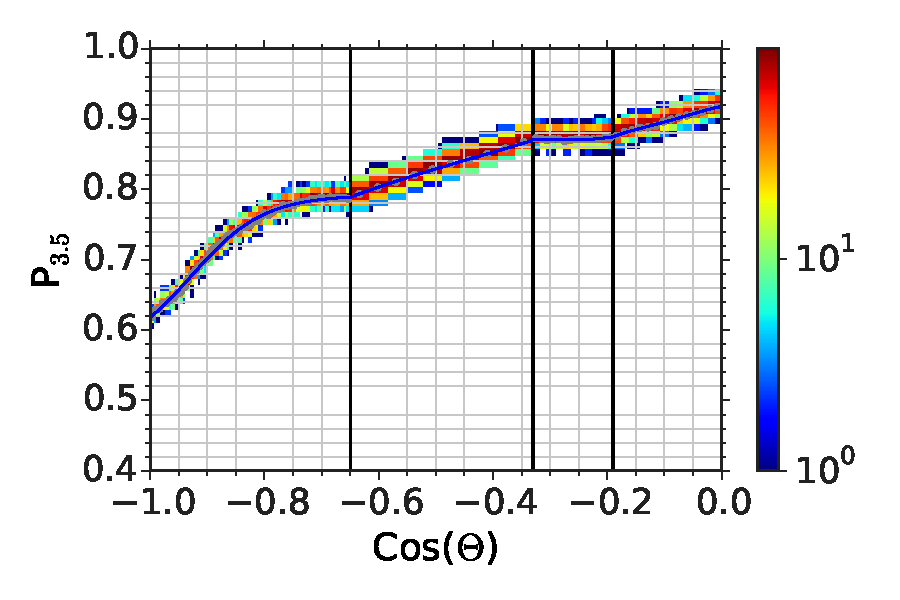
\includegraphics[width=0.45\textwidth]{fig/P3p5param_862_gamma2.pdf}}
\subfloat[Testing the 
parameterization with a second 
dataset.\label{fig:P3p5param_862_gamma2_quality}]{%
 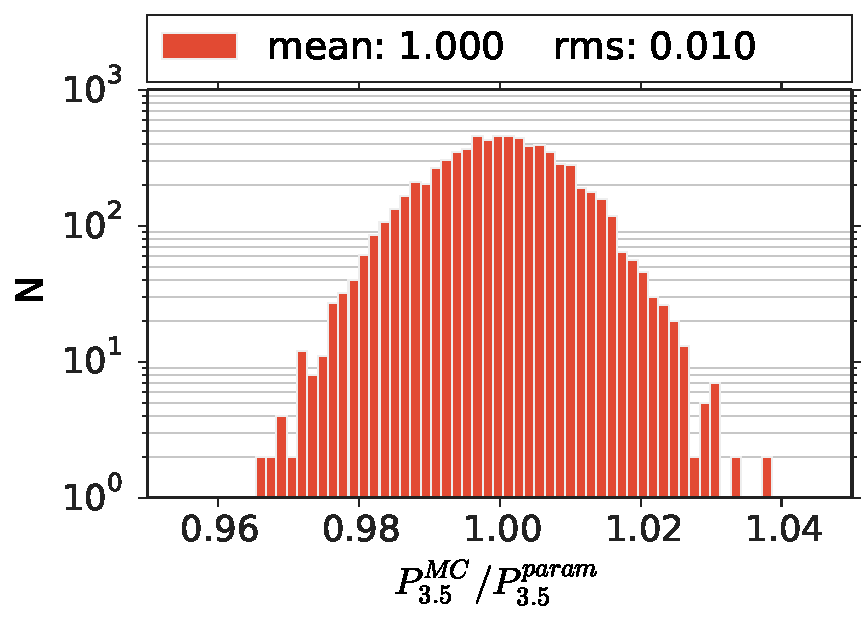
\includegraphics[width=0.45\textwidth]{fig/P3p5param_862_gamma2_quality.pdf}}
\caption{IC86-2 season: The probability of neutrino events to be within 3.5\% 
of each other and the dependency on the cosinus of the GRB zenith angle. The 
blue line represents the parameterization (left). Using a second set of 
simulated GRBs, a histogram 
of the ratio between the calculated probabilities based on all events in 
the zenith bands and the parametrized values is shown (right). The maximum 
deviation 
is about 4\%.}
\end{figure}
The quality of the parameterization can be examined in Fig. 
\ref{fig:P3p5param_862_gamma2_quality}. The overall result is still very 
satisfying though the root mean square is with 0.01 instead of 0.003 larger as 
is the maximum deviation of about 4\% instead of 1\%. However, the 
probabilities $P_{3.5^\circ}^\text{MC}$ in the second control dataset are 
not based on all events within the zenith region in this test. Instead, a 
random selection of 4000 events was used as well leading to possible 
fluctuations of the comparison points compared to the optimal value based on all 
events.
% enabling the comparison of the 
% parametrized value to a deviation of the optimal value based on all events. 
Thus, the slightly worse but still good result is explained and the 
parameterization will be used.

The final probability per zenith direction is not dependent on the absolute 
normalization of the flux as it cancels in equation \ref{eq:P3p5}, but on the 
chosen OFU cuts and the spectral shape. The season and the signal spectrum
define the amount 
events of different energies contribute to the calculation. Therefore, the 
probability is parametrized once per season and spectral index $\gamma$ and is 
then used for all GRB models. The root-mean-square suffers by about 0.1 - 0.2 
percentage points in comparison to individual parameterizations per season, 
$\gamma$ and GRB model and is considered acceptable.

The fitted values to the free parameters in Eq. \ref{eq:Ptanh} and 
\ref{eq:PPoly} as well as the break points between the different regions are 
listed for all season - spectra combinations in table \ref{tab:P3p5fitvalues}.

\begin{table}[h]
  \centering
  \begin{tabular}{r|c|r||l|l|r|l|l|l|l}
season  &  $\gamma$ & region & $b_i$ & a & b & c 
& d & e & f \\
\hline\hline
IC86-1 & 2 & I & -1 &0.113& 7.847& -0.923 &  0.680& - & 
-\\
IC86-1 & 2 & II & -0.65 & 1.206 & 2.472 & 7.126 & 9.782 & 
4.855 \\
IC86-1 & 2 & III & -0.33 & 3.257e-02 & -1.455e+01 & -9.1460e+01 
& -2.488e+02 & -2.481e+02 \\
IC86-1 & 2 & IV & -0.21 & 9.198e-01 & 3.415e-02 & -3.649e+00 &  
-2.404e+01 & -5.053e+01 \\
\hline
IC86-2 & 2 & I &  -1 & 0.115 & 7.857 & -0.928 & 0.678 & - 
& -\\
IC86-2 & 2 & II & -0.65 & 1.041 & 0.910 & 2.191 & 2.687 & 
1.140 \\
IC86-2 & 2 & III &  -0.33 & 0.753 & -2.582 & -18.718 & 
-56.052 &  -59.955 \\
IC86-2 & 2 & IV &  -0.19 & 0.918 & 0.156 & -1.679 & 
-14.0167 & -37.505 \\
\hline
IC86-BDT & 2 & I & -1 & 0.056 & 17.705 & -0.923 & 0.598 & - & - 
\\
IC86-BDT & 2 & II & -0.81 & 0.909 & 0.525 & 0.728 & 0.724 & 0.171 \\
\hline
\hline
IC86-1 & 2.3 & I & -1 & 0.121 & 8.142 & -0.915 & 0.649 & - & -\\
IC86-1 & 2.3 & II & -0.66 & 0.699 & -1.484 & -4.571 & -5.137 & -2.116 \\
IC86-1 & 2.3 & III & -0.33 & 0.463 & -7.566 & -51.675 & -149.622 & -156.750 \\
IC86-1 & 2.3 & IV & -0.22 & 0.907 &  0.149 & -1.409 & -6.671 & -9.912 \\
\hline
IC86-2 & 2.3 & I & -1 & 0.127 & 7.667 & -0.924 &  0.640 & - & - \\
IC86-2 & 2.3 & II & -0.66 & 0.843 & -0.357 & -1.481 & -1.560 & -0.640 \\
IC86-2 & 2.3 & III & -0.33 & 2.351e-02 & -1.387e+01 & -8.545e+01 
& -2.300e+02 & -2.273e+02 \\
IC86-2 & 2.3 & IV & -0.21 & 0.904 & 0.169 & -1.130 & -2.400 & 5.261 \\
\hline
IC86-BDT & 2.3 & I & -1 & 0.066 & 18.423 & -0.925 & 0.560 \\
IC86-BDT & 2.3 & II & -0.81 & 0.899 & 0.638 & 1.153 & 1.339 & 0.454 \\
\hline
\hline
IC86-1 & 2.7 & I & -1 & 0.130 & 8.742 & -0.906 & 0.592 & - & - \\
IC86-1 & 2.7 & II & -0.65 & -0.448 & -10.910 & -33.936 & -44.693 & -21.645 \\
IC86-1 & 2.7 & III & -0.32 & 19.454 & 276.583 & 1531.855 & 3754.553 & 3435.745 
\\
IC86-1 & 2.7 & IV &  -0.23 & 0.873 & 0.077 & -2.717 & -9.764 &  -7.907 \\
\hline
IC86-2 & 2.7 & I & -1 & 0.150 & 7.004 & -0.922 & 0.573 & - & - \\
IC86-2 & 2.7 & II & -0.66 & 0.430 & -3.295 & -9.984 & -12.148 & -5.474 \\
IC86-2 & 2.7 & III & -0.33 & 1.965 & 15.083 & 71.629 & 147.549 & 111.037 \\
IC86-2 & 2.7 & IV & -0.22 & 0.872 & 0.236 & -0.210 & 14.100 & 61.454 \\
\hline
IC86-BDT & 2.7 & I & -1 & 0.079 & 18.777 & -0.929 & 0.489 & - & -  \\
IC86-BDT & 2.7 & II & -0.81 & 0.874 & 0.919 & 2.247 & 2.942 & 1.226 \\
  \end{tabular}
  \caption{The fit values to the parameters in functions \ref{eq:Ptanh} and 
\ref{eq:PPoly}. $e$ and $f$ are marked '-' if the first function was used. All 
values have been rounded to the third decimal place. The break points $b_i$ 
denote the left starting point of a region in $\cos \theta_\text{GRB}$.}
  \label{tab:P3p5fitvalues}
\end{table}


% parameterization.]{
% %  \captionsetup{width=.9\textwidth}
%   
% % \caption{}
% % 
% %  \end{minipage}
% %  \begin{minipage}{0.5\textwidth}
% %  \captionsetup{width=.9\textwidth}
% \subfloat[]{
% % \caption{}
% % 
% %  \end{minipage}
% \end{figure}
%explain figure ???
%is delta t really drawn within 0, 100 s? or is max t90? and what is correct?

\paragraph{Doublet Probability}$\;$\\
The probability that two neutrinos coincide as a doublet that triggers OFU is 
then
\begin{equation}
 P_\text{D} = P_{\Delta t} \cdot P_{3.5^\circ}
\end{equation}


\paragraph{P$_{\text{llh}}$}$\;$\\
On average the doublet selection based on time and direction leads to about 50 -
60
doublets per year (depending on season) while only seven alerts can be sent to
the Swift telescope. The
selection of the most signal like doublets is based on the OFU test statistic 
\ref{eq:alert-llh}.
% \begin{align}
%     \begin{split}
%     \lambda = -2 \ln \mathcal{L} &= \frac{\Delta\Psi^2}{\sigma_q^2} + 2 \ln(2
% \pi \sigma_q^2) \\
%                               &- 2 \ln\left( 1 -
% e^{\frac{-\theta_A^2}{2\sigma_w^2}}\right) 
%                               + 2 \ln\left( \frac{\Delta T}{\unit[100]{s}}
% \right)
%     \end{split}
%   \label{eq:alert-llh}
% \end{align}
% where the time between the neutrinos in the multiplet is denoted as $\Delta T$
% and their angular separation as $\Delta\Psi$. $\sigma_q^2 = \sigma_1^2 +
% \sigma_2^2$ and $\sigma_w^2 = \left(1/\sigma_1^2 + 1/\sigma_2^2\right)^{-1}$
%  are the combined uncertainties of the directional
% reconstruction errors $\sigma_1$ and $\sigma_2$ of the two neutrino events.
% $\theta_A$ corresponds to the (circularized) angular radius of the field
% of view (FoV) of the follow-up telescope (set to $0.5^\circ$ for Swift). A cut 
% value $\lambda_\text{cut}$ was chosen each season to filter out the best nine 
% alerts (Table \ref{tab:llh cut values}).
% 
% \begin{table}[h]
%   \centering
%   \begin{tabular}{l|c|c|c}
%    Season & IC86-1 & IC86-2 & IC86-BDT \\
% \hline
%    cut value & -8.8 (check) & -8.8 & -9.41 \\
%   \end{tabular}
%   \caption{The cut values on the likelihood to filter down the number of
% background doublets to less or equal than 9.}
%   \label{tab:llh cut values}
% \end{table}

The test statistic is calculated for all event pairs that pass the condition of
being reconstructed within $3.5^\circ$ (denoted as $| \; \Delta \Psi(i, j) \leq 
3.5^{\circ}$). They are given a total weight by multiplying the individual 
event weights.
The time difference is randomly drawn
with $\Delta T \in [0, 100]$ s and weighted according to an exponential decay
(Eq. \ref{eq:lum_vs_time}) introducing a dependency on $t_{90}$
(Eq. \ref{eq:ToyMC_tau}).
The probability that
a GRB doublet will pass the cut $\lambda_\text{cut}$ is determined by taking 
the ratio of the weight sum of doublets passing $\lambda_\text{cut}$ and the 
weight sum of all considered doublets.
\begin{equation}
\label{eq:Pllh}
 P_\text{llh} = \frac{\sum_{i} \sum_{j=i+1} w_i \cdot w_j \; | \; \lambda(i, j)
\leq \lambda_\text{cut} \; | \; \Delta \Psi(i, j) \leq 3.5^{\circ}}{\sum_i
\sum_{j=i+1} w_i \cdot w_j \; | \; \Delta \Psi(i, j) \leq 3.5^{\circ}}
\end{equation}

% \begin{figure}[h]
%  \begin{minipage}{0.5\textwidth}
%  \captionsetup{width=.9\textwidth}
%   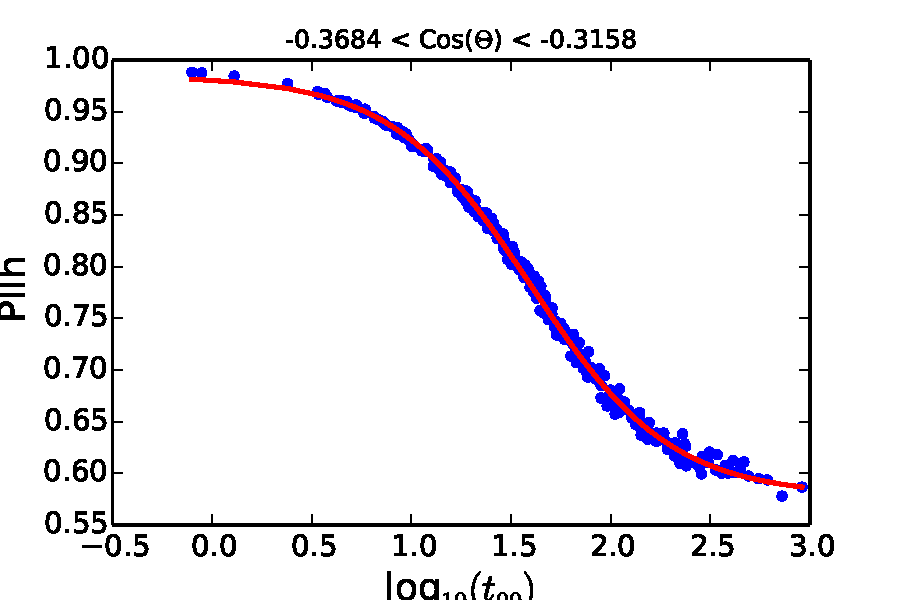
\includegraphics[width=\textwidth]{fig/Pllhparam.pdf}
% \caption{The probability of neutrino events to pass the cut on the test
% statistic and the dependency on the logarithm of the $t_{90}$ value for a
% certain cosinus bin. The red line represents the parameterization.}
% \label{fig:Pllhparam}
%  \end{minipage}
%  \begin{minipage}{0.5\textwidth}
%  \captionsetup{width=.9\textwidth}
%   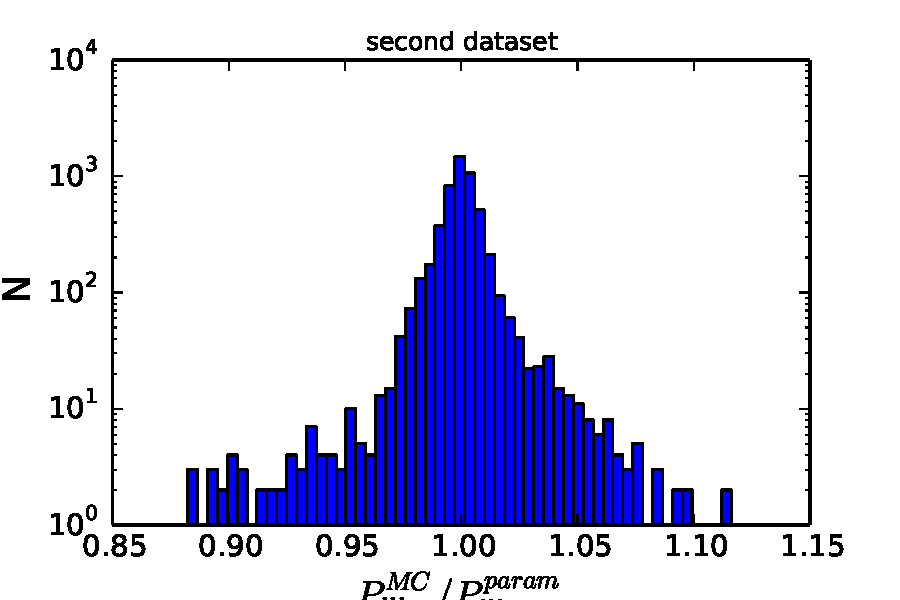
\includegraphics[width=\textwidth]{fig/Pllhparam_quality.pdf}
% \caption{Using a second dataset, a histogram of the ratio between the calculated
% and parametrized values is shown. Most GRBs fall within 5\% derivation while
% some outliers differ up to 12\%.\\}
%  \end{minipage}
% \end{figure}



The parameterization of $P_\text{llh}$ is more complicated than
$P_{3.5^\circ}$. The test statistic depends not only on properties of the 
simulated neutrino events like the zenith angle
% and thus the zenith angle
but on the time window 
between two neutrinos and, therefore, on $t_{90}$. The data is split 
into 180 cosinus bins
and the probability is fitted against the logarithm of the drawn $t_{90}$ (Eq.
\ref{eq:t90dist} and \ref{eq:t90earth}) value for each bin. The amount of 180 
bins is a compromise between precision and needed computational power. The 
probability changes rapidly near the pole requiring a high 
number of bins. In return, many simulated GRBs are needed to facilitate a good 
parameterization representing various GRBs per bin and $t_{90}$ value.

\begin{figure}[h]
 \centering
 \captionsetup{width=0.85\textwidth}
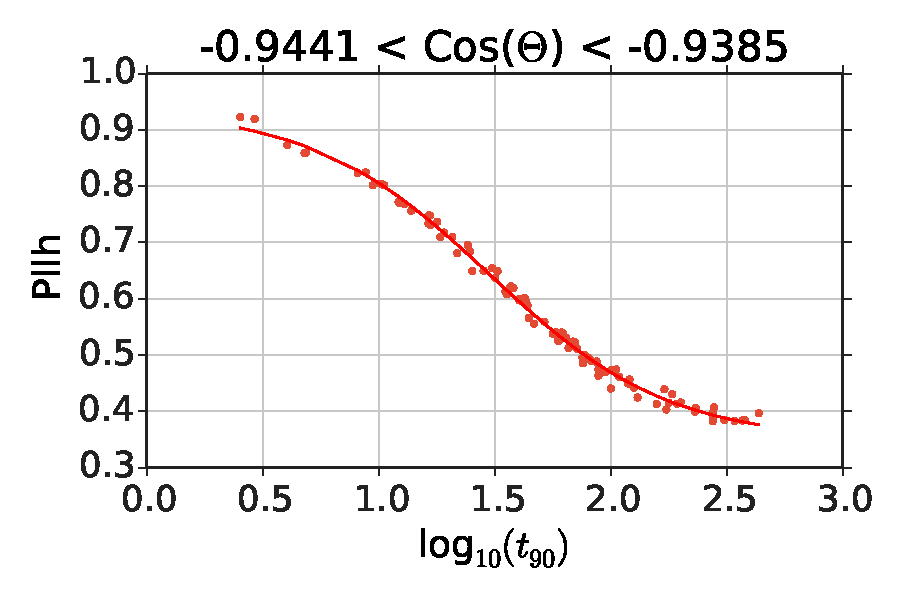
\includegraphics[width=0.6\textwidth]{fig/Pllh_example_g2_bdt.pdf}

\caption{The probability for a doublet to pass 
the cut on the likelihood (Eq. 
\ref{eq:alert-llh}) vs the logarithm of 
$t_{90}$. As an example, the cosinus bin of $-0.9441 < \cos \theta_\text{GRB} 
< -0.9385$ is shown. The red dots represent values calculated according to Eq. 
\ref{eq:Pllh} for drawn GRBs. The red line is a fit to these values. 
\label{fig:Pllh_example_g2_bdt}}
\end{figure}

An example based on a dataset for the IC86-BDT season and a spectral index of 
$\gamma=2$ is shown in Figure
\ref{fig:Pllh_example_g2_bdt} displaying individual calculated probabilities of 
GRBs as red dots and a fit to these points as a function of the logarithm of 
$t_{90}$. The fit is based on Eq. \ref{eq:Ptanh}. Such a fit is done for each 
bin in $\cos \theta_\text{GRB}$ and for each season - $\gamma$ combination in 
turn. Due to the large number of plots only an example is displayed.

The quality of the parameterization can be judged by examining Figure 
\ref{fig:Pllhparam_bdt_gamma2_quality}. The parameterization was applied to a 
second dataset for which the probability was calculated according to 
\ref{eq:Pllh} for all events within the zenith band. The ratio of calculated 
and parametrized values are displayed in the histogram. Both the root mean 
square with $0.006$ and the maximum deviation with about 3 
percentage points are satisfactory small. 

%proof that outliers average out???
%where do they lie??? which GRBs???
\begin{figure}[h]
\centering
 \captionsetup{width=.85\textwidth}
%  \captionsetup{margin=0pt}
\subfloat[Probability to pass 
likelihood cut.\label{fig:Pllhparam_bdt_gamma2_quality}]{%
 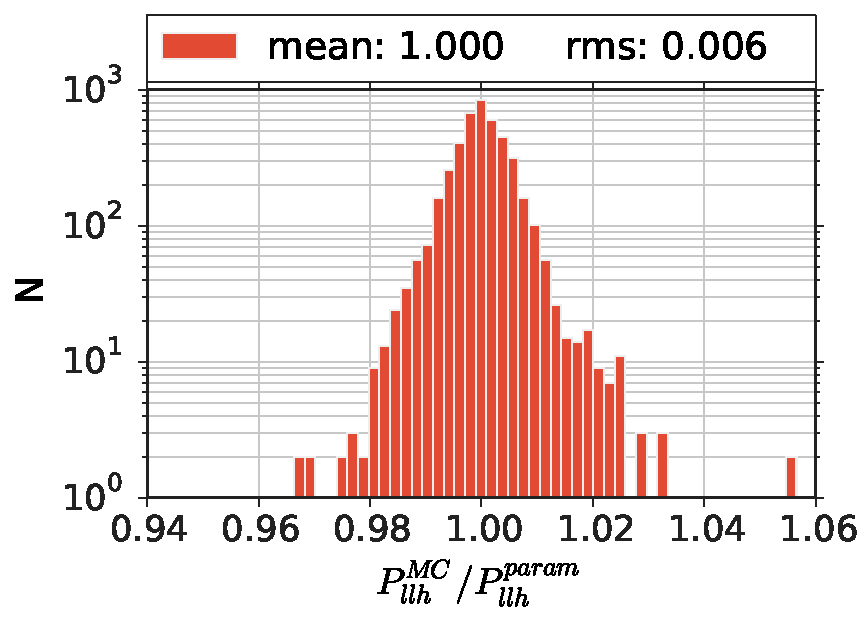
\includegraphics[width=0.45\textwidth]{fig/Pllhparam_bdt_gamma2_quality.pdf}}
 \subfloat[Probability for a GRB to be within Swift FoV. 
\label{fig:PonSparam_bdt_gamma2_quality}]{%
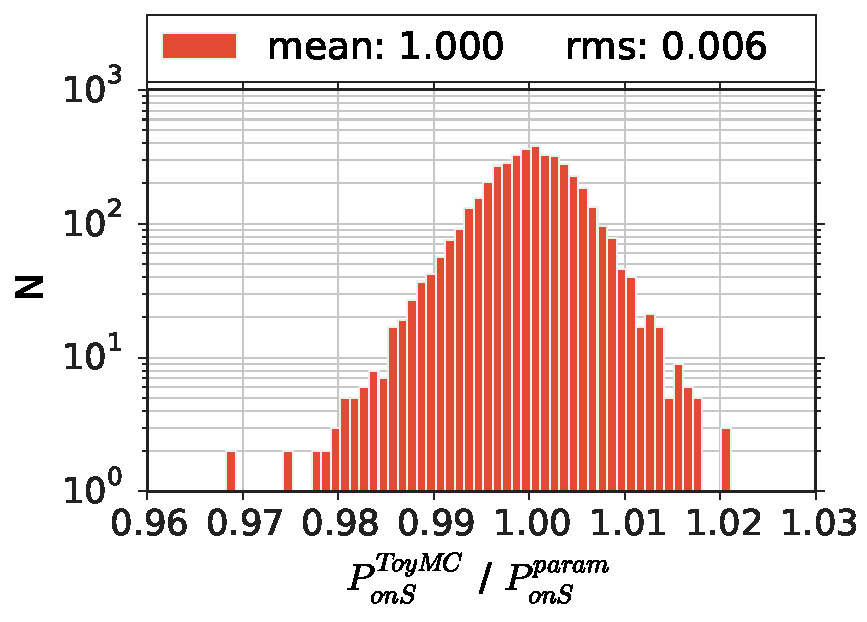
\includegraphics[width=0.45\textwidth]{fig/PonSparam_bdt_gamma2_quality.pdf}}
\caption{Season IC86-BDT: Using a second set of simulated GRBs, a histogram 
of the ratio between the calculated probabilities and the parametrized values 
is shown. The maximum deviation 
is of about 2 percentage points.}
\end{figure}


\paragraph{P$_\text{onS}$}$\;$\\
The Optical Follow-Up program calculates the weighted mean direction from all
events contributing to a multiplet using the Cramer Rao error as weights. For a 
source to be detectable
with Swift, its
direction must be within 0.5 degrees of the true source direction. The
probability $P_\text{onS}$ for two events to point back to the source well
enough is given by
the ratio of the sum over the event weight products fulfilling the condition
and the sum over all event weight products:
\begin{equation}
P_\text{onS} = \frac{\sum_i \sum_{j=i+1} w_i \cdot w_j |
\Psi_{\text{weighted mean}}(i, j) - \Psi_{GRB} \leq 0.5^{\circ} \; | \;
\lambda(i, j)
\leq \lambda_\text{cut} \; | \; \Delta \Psi(i, j) \leq 3.5^{\circ}}{\sum_i
\sum_{j=i+1} w_i \cdot w_j \; | \; \lambda(i, j)
\leq \lambda_\text{cut} \; | \; \Delta \Psi(i, j) \leq 3.5^{\circ}} 
\end{equation}
Only events passing the conditions $\Delta \Psi(i,j) \leq 3.5^\circ$ and 
$\lambda(i, j) \leq \lambda_\text{cut}$ are considered.
The parametrization is performed using the methods used and described for 
$P_\text{llh}$ leading to a similar quality as can be judged with the help of 
Figure 
\ref{fig:PonSparam_bdt_gamma2_quality}.

\paragraph{Alert Probability}$\;$\\
The probabilities described in this section until now are conditional and can 
be 
combined via multiplication according to the Base Theorem and the probability 
that two neutrinos are detected, trigger the Swift Follow-Up and that the 
source is within Swifts FoV is
\begin{equation}
 P_\text{Alert} = P_{2\nu} \cdot P_D \cdot P_\text{llh} \cdot P_\text{onS}.
\end{equation}
$P_\text{onS}$ can be set to one if only the probability to have a Swift
alert is of interest.

Given these parameterizations, a big number of usually around five 
million GRBs are thrown to create a sample representing the complete redshift 
and luminosity range.

%more detail? plot?


\subsubsection{Probability to Detect a GRB}
The previous section described a simplified case of only two neutrinos. 
However, if $\mu$ neutrinos are expected per GRB there is a chance to see more 
than two neutrinos. There are two trigger conditions for a Swift alert. 
Usually, one doublet is 
detected and passes the Swift cut on the OFU test statistic as 
well. However, there is the 
possibility of a 'higher multiplet' as well which we define as an alert of at 
least three neutrinos.

In both cases the number of possible 
doublets and the probability of them to be detected needs to be calculated. If 
$N$ neutrinos are detected, the first neutrino can be part of a doublet with 
$N-1$ partners, while the second neutrino can combine with $N-2$ partners. The 
general formula describing the number of possible combinations is the Gaussian 
Sum Formula
\begin{equation}
 d = 1 + 2 + ... + (x-1) + x= \frac{x^2 + x}{2}.
\end{equation}
Two neutrinos are needed to form a doublet, leading to the substitution $N = 
x-1$. The number of possible doublets is then 
\begin{equation}
 d = \frac{N^2 - N}{2}.
\end{equation}
with each doublet having a probability $P_D$ to pass the time window and 
angular separation cuts. The probability for this to happen $k$ out of $d$ 
times is given by the binomial distribution
\begin{equation}
 P_\text{bin} ( k, d(N), P_D) =  \binom{d}{k} \cdot P_{D}^k \cdot 
(1 - P_{D})^{d-k} = \binom{0.5 (N^2 - N)}{k} \cdot P_{D}^k \cdot 
(1 - P_{D})^{0.5(N^2 -N) -k}
\end{equation}

The correct probability to see exactly one doublet to is determined by 
multiplying the probability to see $N$ neutrinos and the probability of these 
$N$ 
neutrinos to form exactly one doublet for all $N \geq 2$
\begin{equation}
 P_\text{1 Doublet} = \sum_{N=2}^{N_\text{max}} P_\text{Poisson}(N, 
\mu) \cdot P_\text{bin} (1, d(N), P_D)
\end{equation}
$N_\text{max}$ is chosen to achieve a precision in the order of $10^{-6}$.
The probability that one doublet passes the likelihood cut as well is given by
\begin{equation}
 P_\text{1 Swift Doublet} = P_\text{1 Doublet} \cdot P_\text{llh}
\end{equation}

The second channel is triggered when at least three neutrinos 
result in at least two doublets.
\begin{equation}
 P_\text{Multiplet} = \sum_{n=3}^{n_\text{max}} P_\text{Poisson}(n, 
\mu) \cdot [1 - P_\text{bin} (0, d(n), P_D) - P_\text{bin} (1, 
d(n), P_D)]
\end{equation}

These definitions can be used to calculate the probability to detect a specific 
GRB. Generating $N_\text{gen} = 5\cdot10^6$ GRBs, the number of GRBs that are 
expected to be detected
in a specific channel is the sum over all probabilities, e.g. for higher 
multiplets
\begin{equation}
 N_\text{GRB} / yr = \sum_{i=0}^{N_\text{gen}} P_{\text{multiplet},i} \cdot 
\frac{N_\text{GRB, yr}}{N_\text{GRB, gen}}
\end{equation}
The ratio at the end is necessary to renormalize the result to the expected 
number of 
GRBs per year $N_\text{GRB, yr}$.

This concludes the description of the Toy Monte Carlo to calculate the expected 
number of expected signal alerts for different spectra and GRB models. The 
following section describes how to use the background and signal expectations 
 to calculate a test statistic. It will be used to draw limits on the 
contribution of transients to the HESE flux.

\newpage
\section{Significance and Limit calculation}
\label{sec:limits}
This 
section will describe the test statistic to evaluate the conformity with 
background of the measured alerts.
% if the measured alerts are 
% background conform or can be attributed to a signal source.
The test statistic is based on multiplying the p-values of different 
components which can be separated into two categories: the pure number of 
alerts and the probability that doublets stem from background.

The Optical Follow-Up was designed with the expectation that most of the alerts 
will be triggered due to background events of atmospheric neutrinos. An excess 
of detected multiplets in comparison to the expected background 
average can indicate a possible signal contribution. 

Given the average 
background expectation (Section ???) $\mu_{k,b}$ for multiplets with 
multiplicity $k$, the probability to see $N_k$ or more alerts during one 
season is
\begin{equation}
 P(N_k, \mu_k) = \sum P_\text{Poisson} = \sum_{i=N_k}^\infty 
\frac{\mu_k^i}{i!}\exp^{-\mu_k}.
\end{equation}
The sum is aborted when a precision of $10^{-6}$ is reached.
The probabilities for the different multiplicities $k$ and seasons $i$ are then 
multiplied to form the test statistic $\lambda_{na}$ to evaluate the number of 
alerts
\begin{equation}
\label{eq:test_statistic}
 \lambda_{na} \left(N_k^i, \mu_{k,b}^i \right) = \prod_{k=2}^\infty \prod_i 
P(N_k^i, 
\mu_{k,b}^i).
\end{equation}

The second component is only valid for doublets as higher multiplicities are 
automatically considered true alerts. The OFU system generates up to about 50 
doublets per year of which only seven can be sent to Swift. The down selection 
is based on the OFU test statistic (Section ???) separating the more signal 
like and the more background like doublets. For each doublet an OFU test 
statistic value is drawn and compared to the background distribution to 
calculate the p-value $p_{j, i}^{ofu}$. The p-values of all doublets can not 
simply be multiplied as the number of doublets would influence the significance 
of the test statistic. E.g. three background doublets would form a smaller 
overall p-value $O(10^{-3})$ than one signal doublet $O(10^{-1})$. A combination 
of all $p_{j,i}^{ofu}$ was chosen to keep the total contribution in the same 
order of magnitude independent of the number of doublets.
%order as the contributions of the amount of multiplets per multiplicities and 
%season $P(N_k^i, \mu_{k,b}^i)$ by multiplying i
All $p_{j,i}^{ofu}$ are multiplied and 
the ${N_2^i}^{th}$ square root is taken of the product with $N_2^i$ being the 
number of considered 
doublets of season $i$
\begin{equation}
\label{eq:lambda_ofu}
 \lambda_\text{ofu} = \prod_i \sqrt[N_2^i]{\prod_{j=1}^{N_2^i} p_{j,i}^{ofu}}
\end{equation}
Calculating $p_{j,i}^{ofu}$ is based on several steps. The OFU test statistic 
distribution differs slightly for different zenith regions. To evaluate the 
correct test 
statistic a zenith value is drawn for each doublet according to the squared 
singlet rate (Figure \ref{fig:cos_zen_prob_dens_bg_IC86_BDT}, 
\ref{fig:cos_zen_prob_dens_sg2p3_IC86_BDT}). 

\begin{figure}[h]
\centering
 \captionsetup{width=.85\textwidth}
%  \captionsetup{margin=0pt}
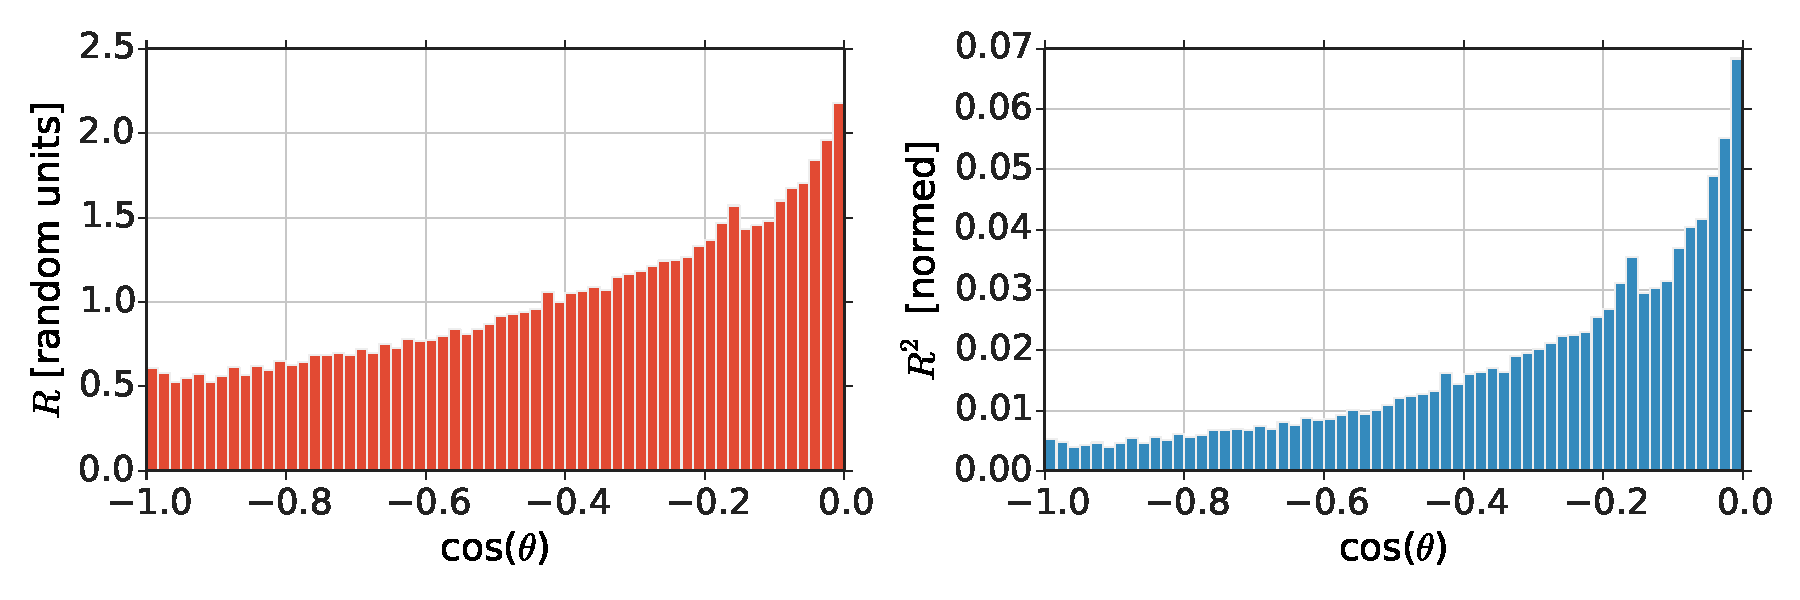
\includegraphics[width=0.85\textwidth]{%
fig/cos_zen_prob_dens_bg_IC86_BDT.pdf}
 \caption{The plots show the cosinus zenith distribution for background of the 
IC86-BDT season. The left plot depicts the singlet rate in random units and the 
right plot is the probability density function of the doublet distribution 
(singletrate squared)}
\label{fig:cos_zen_prob_dens_bg_IC86_BDT}
\end{figure}

\begin{figure}[h]
\centering
 \captionsetup{width=.85\textwidth}
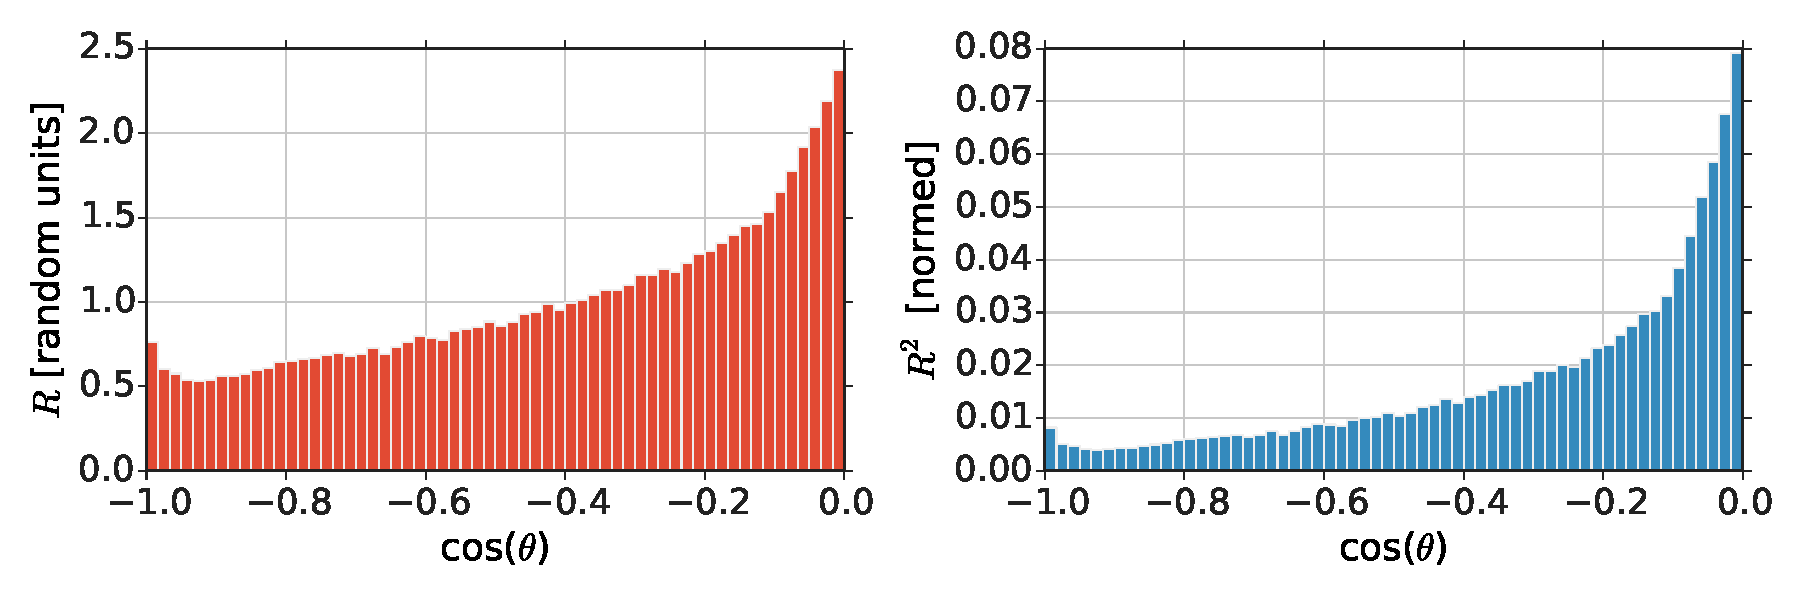
\includegraphics[width=0.85\textwidth]{%
fig/cos_zen_prob_dens_sg2p3_IC86_BDT.pdf}
\caption{The plots show the cosinus zenith distribution for signal with a 
spectral index of $\gamma=2.3$ of the 
IC86-BDT season. The left plot depicts the singlet rate in random units and the 
right plot is the probability density function of the doublet distribution 
(singletrate squared)}
\label{fig:cos_zen_prob_dens_sg2p3_IC86_BDT}
\end{figure}
The northern sky was divided 
into twenty even regions in $\cos(\theta)$ and the probability density 
functions of the OFU test statistic were created for background and signal of 
all considered spectra for all seasons in each region. An example is shown 
in Figure \ref{fig:ofu_teststat_zone00_IC86_BDT_bg_g2p3} for the first zone 
from the pole for the IC86-BDT season. Using the zenith value the correct OFU 
test statistic probability density function is chosen to draw a test statistic 
value. As the probability to have a Swift doublet is already included in 
calculating the expected number of doublets $\mu_{2}^i$, the test statistic 
value must be smaller than the Swift cut of the season. The chosen value is 
then compared to the cumulative background distribution (Figure 
\ref{fig:ofu_teststat_zone00_IC86_BDT_bg_cum}) and the p-value is extracted.

\begin{figure}[h]
\centering
 \captionsetup{width=.4\textwidth}
%  \captionsetup{margin=0pt}
 \subfloat[The probability density functions of the OFU test statistic 
(background and signal with a spectral index of $\gamma=2.3$) for the first 
region starting from the pole for the IC86-BDT season. 
\label{fig:ofu_teststat_zone00_IC86_BDT_bg_g2p3}]{%
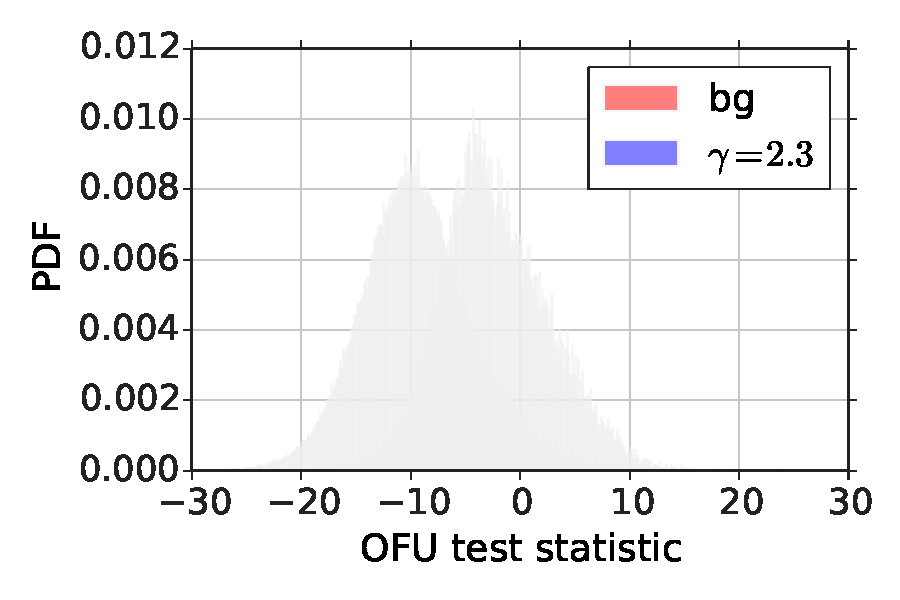
\includegraphics[width=0.45\textwidth]{%
fig/ofu_teststat_zone00_IC86_BDT_bg_g2p3.pdf}}
\subfloat[The cumulative 
distribution of the background 
OFU test statistic for the 
IC86-BDT season.\label{fig:ofu_teststat_zone00_IC86_BDT_bg_cum}]{%
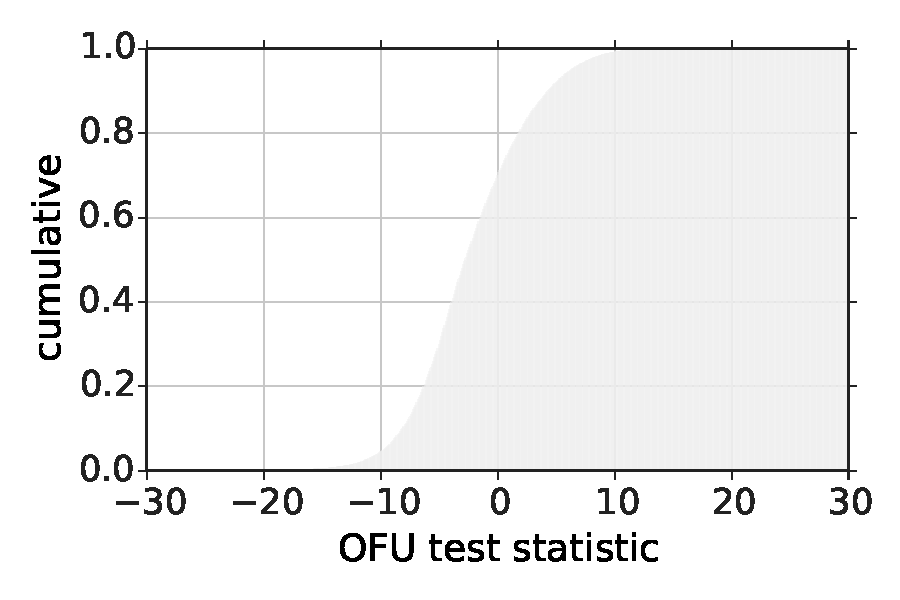
\includegraphics[width=0.45\textwidth]{%
fig/ofu_teststat_zone00_IC86_BDT_bg_cum.pdf}}
\end{figure}

The complete test statistic is the combination of both components
\begin{equation}
\label{eq:lam_total}
 \lambda = \lambda_{na} \cdot \lambda_\text{ofu}
\end{equation}


The final significance and limit calculation is based on running pseudo 
experiments. To evaluate the 
agreement of the measured alerts with a pure background hypothesis, the average 
background expectation $\mu_{k, b}^i$
per season $i$ and multiplicity $k$  is used to draw a number of 
detected multiplets $N_k^i$ according to a Poisson distribution. 
For all $N_2^i$ doublets, $p_{j,i}^{ofu}$ is calculated. 
In total, 
$10^6$ experiments are performed per season and the resulting 
 test statistic values are compared to the measured result ($\lambda_m$). The 
p-value is the fraction of experiments with worse agreement to the background 
hypothesis ($\lambda < \lambda_m$).


Similarly, a signal hypothesis can be tested. The GRB Toy Monte Carlo is used 
to estimate the average number of expected multiplets $\mu_{k,s, \gamma}^i$ for 
a 
specific model and $N_{k,s, \gamma}^i$ values are again generated according to 
the 
Poisson  distribution. The number of alerts $N_{k,s+b}^i$ is the
combination of background and signal alerts
\begin{equation}
 N_{k,s+b}^i = N_{k,s}^i + N_{k,b}^i.
\end{equation}
The influence of the OFU test statistic (Eq. \ref{eq:lambda_ofu}) is 
\begin{equation}
 \lambda_\text{ofu} = \prod_i \sqrt[N_{2,s+b}^i]{\prod_{j=1}^{N_{2,b}^i} 
p_{j,i,b}^{ofu} \cdot \prod_{j=1}^{N_{2,s}^i}
p_{j,i,s}^{ofu}}
\end{equation}

Again, $10^6$ experiments are performed per season and GRB 
model and the test statistic (Eq. \ref{eq:lam_total})
% $\lambda\left(N_{k,s+b}^i, \mu_{k,b}^i \right)$
evaluated. A model can be ruled 
out at 90\% confidence level if 90\% of the experiments show a worse agreement 
with the background only hypothesis than the actual experimental results.
An example is shown in Figures \ref{fig:test_statistic} and 
\ref{fig:test_statistic_cumulative}.
\begin{figure}[h]
\centering
 \captionsetup{width=.9\textwidth}
%  \captionsetup{margin=0pt}
\subfloat[Differential distribution\label{fig:test_statistic}]{%
 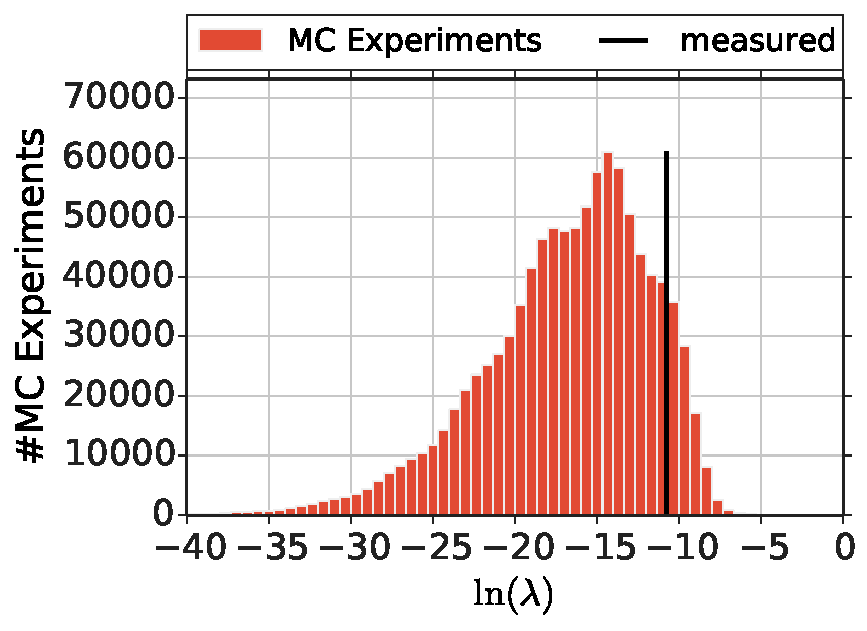
\includegraphics[width=0.45\textwidth]{fig/test_statistic.pdf}}
 \subfloat[cumulative distribution\label{fig:test_statistic_cumulative}]{%
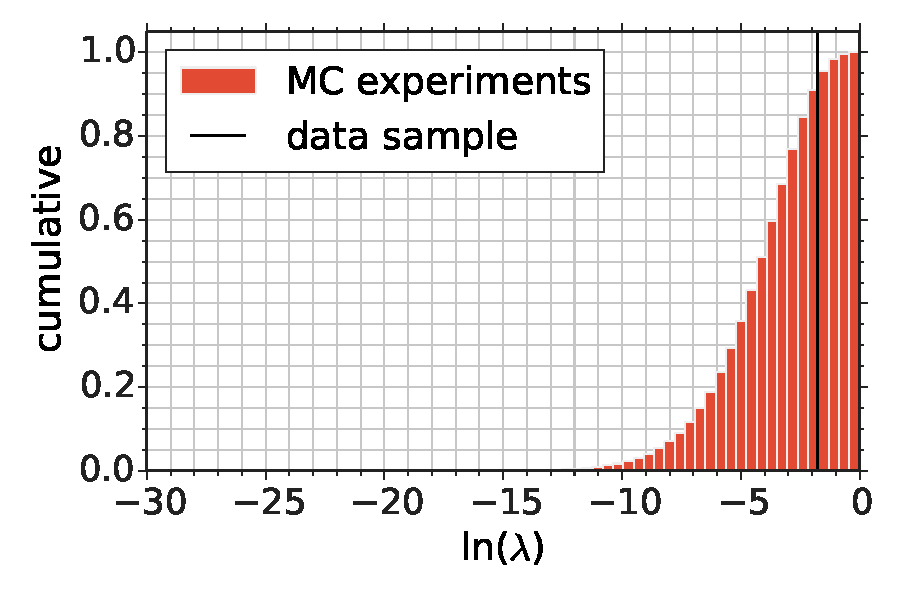
\includegraphics[width=0.45\textwidth]{fig/test_statistic_cumulative.pdf}}
\caption{$10^6$ experiments were thrown and the 
test statistic $\lambda$ was calculated according 
to equation \ref{eq:test_statistic}. In read is the differential
distribution of the Monte Carlo experiments while 
the black line represents the detected value. About 90\% of the experiments 
have a worse agreement with the background only hypothesis.}
\end{figure}

% % in thesis write abortion of quadruplets in bg//????
% 
% % explain: more multiplets than expected. might be due to signal. test hypothesis 
% % that it is pure background. -> test how many experiments are less background 
% % like than measured. -> pvalue
% % 
% % the other idea: we have a model giving us a signal leading to a certain number 
% % of multiplets. if high enough, than having measured to few -> model can be 
% % excluded. for that u_k stays for background only in test statistic but is 
% % tested with N_k = N_k,s + N_k,b. hence. the signal plus bg is tested against 
% % background case. if in 90 \% of the cases the lambda is smaller means that 
% % measurement agrees better with bg than 90 \% of the experiments. only 10 \% 
% % better with bg. model can be ruled out. 
% % 
% % problem: I think that current setup uses signal + bg in lambda. Is that true. 
% % How do I then get the same exclusion regions as nora? in that case shouldn't be 
% % 0.1 be the 90\% exclusion?
% 
% 
% In this section the test test statistic and the Toy Monte Carlo are explained 
% that are used to test the hypothesis that the experimental data is pure 
% background and to limit the possible contribution of a neutrino signal due to 
% a 
% transient source.
% 
% The Toy Monte Carlo runs $10^6$ experiments drawing a number of alerts $N_k$ 
% according to a Poisson distribution with a given mean expectation of $\mu_k$.
% % Given an average expectation value $\mu_k$ of alerts with a multiplicity $k$, 
% % a 
% % number of alerts $N_k$ are drawn according to the Poisson distribution $10^6$ 
% % times for each season.
% For each experiment 
% \begin{equation}
%  P(N_k, \mu_k) = \sum P_\text{Poisson} = \sum_{i=N_k}^\infty 
% \frac{\mu_k^i}{i!}\exp^{-\mu_k}
% \end{equation}
% describes the probability to detect $N_k$ or more alerts. The sum is aborted 
% when a precision of $10^{-6}$ is reached. All experiments are combined to a 
% distribution of the test statistic
% \begin{equation}
%  \lambda_\nu = \prod_{k=2}^\infty \prod_i P(N_k^i, \mu_k^i)
% \end{equation}
% in which the probabilities of each contributing seasons are multiplied per 
% multiplicity and then similarly combined with the probabilities of the 
% different types of multiplets.
% 
% In the previous section the methods to calculate an average background 
% $\mu_k^{BG}$ and a signal expectation $\mu_k^{S}$ for alerts with the 
% multiplicity $k$ has been described. 
% To limit a possible signal flux, the average expectation value is set to a 
% combination of background and signal expectation
% \begin{equation}
%  \mu_k = \mu_k^S + \mu_k^{BG}
% \end{equation}
% and the test statistic is calculated $10^6$ times as explained above and 
% compared to the value for the measured multiplets rate $\lambda_m$. A model 
% can be ruled out with the probability of the fraction $x$ of experiments 
% which show a worse agreement with the hypothesis, e.g. with a smaller test 
% statistic value than the measured data.
% An example is shown in Figures \ref{fig:test_statistic} and 
% \ref{fig:test_statistic_cumulative} in which the signal hypothesis is ruled out 
% at a 90\% confidence level.
% \begin{figure}[h]
% \centering
%  \captionsetup{width=.4\textwidth}
% %  \captionsetup{margin=0pt}
% \subfloat[\label{fig:test_statistic}]{%
%  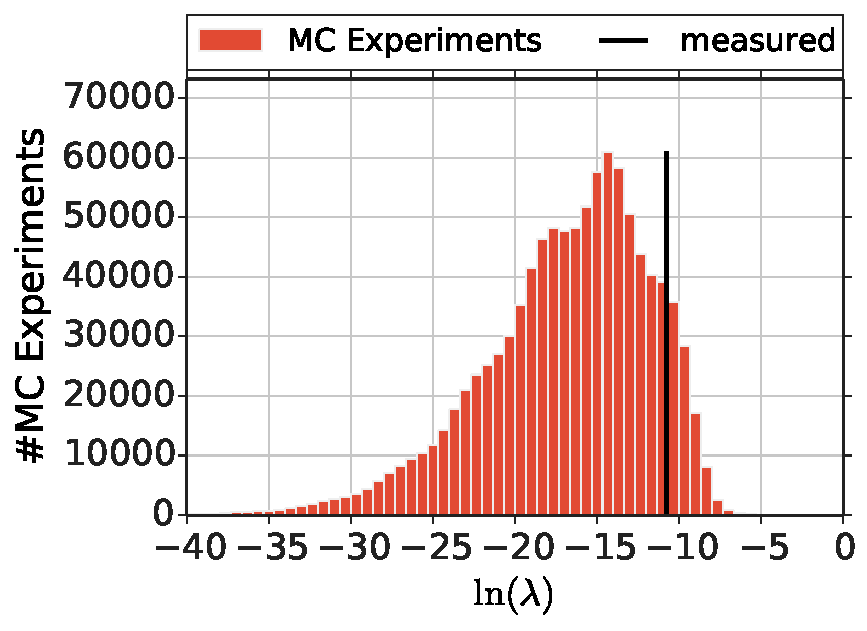
\includegraphics[width=0.45\textwidth]{fig/test_statistic.pdf}}
%  \subfloat[ 
% \label{fig:test_statistic_cumulative}]{%
% 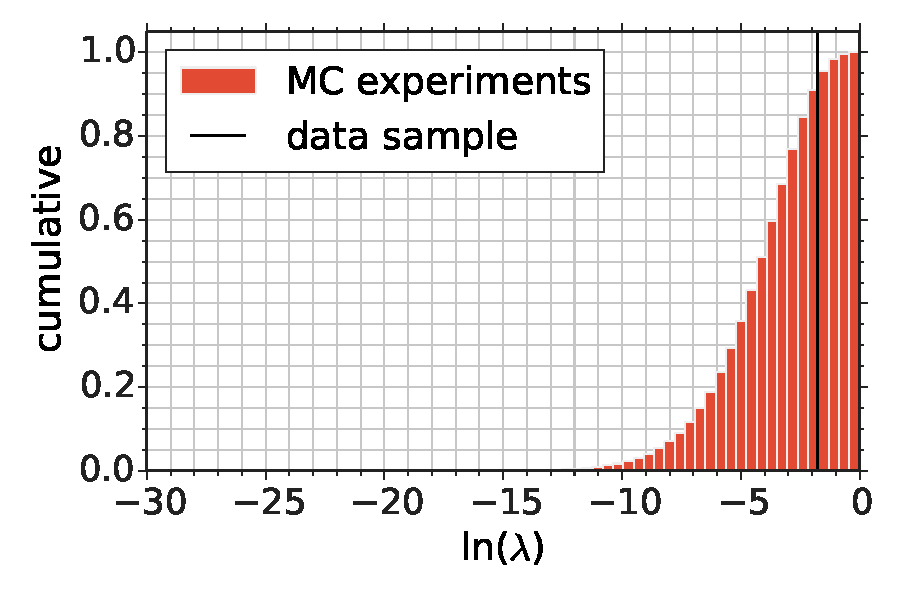
\includegraphics[width=0.45\textwidth]{fig/test_statistic_cumulative.pdf}}
% \end{figure}
% 
% Similarly, the sensitivity to the pure background hypothesis can be tested by 
% setting 
% \begin{equation}
%  \mu_k = \mu_k^{BG}
% \end{equation}
% and rerunning the Toy Monte Carlo. A possible signal contribution becomes 
% likely if few experiments have a worse agreement with the background assumption 
% meaning a value less than the measured 
% 
%  significance  The p-value is the 
% fraction of experiments that agree worse with this hypothesis than the data 
% taken, i.e. the experiments with a value smaller than $\lambda_m$.

\section{Results}
\label{sec:Results}
The whole simulation setup and the methodology described in the last sections 
can be used to draw limits on the contribution of GRBs and other short 
transients to the detected diffuse high energy neutrino flux (HESE flux). The 
results and the impacts of different models is described in this section.

\subsection{Limits on Contribution to the HESE Flux by Transient Neutrino 
Sources}
In chapter \ref{sec:limits}, the methodology to calculate limits on the 
contribution of a transient population to the HESE flux was described. The 
pseudo experiments need to be repeated for each different signal model. The 
result for a spectrum with $\gamma=2.3$, 3000 GRBs per year and a fraction of 
5.95\% of the HESE flux to be produced by these GRBs are shown in Figures 
\ref{fig:test_statistic} and \ref{fig:test_statistic_cumulative}. The GRB rate 
density is not a known value but a parameter. To calculate the p-value for 
different rate densities and fraction of contribution to the HESE flux, the 
signal expectation $\mu_s$ can be scaled by 
\begin{equation}
 \hat{\mu_s} = \mu_s \cdot \zeta \frac{3000\mathrm{ 
GRBs/yr}}{N_\mathrm{GRBs/yr}}
\end{equation}
with $\zeta$ being the contribution to the total HESE flux. By doubling the 
number of GRBs, the neutrino flux per GRB gets reduced by half, leading to 
softer limits.

\begin{figure}[h]
 \centering
 \captionsetup{width=.9\textwidth}
%  \captionsetup{margin=0pt}
 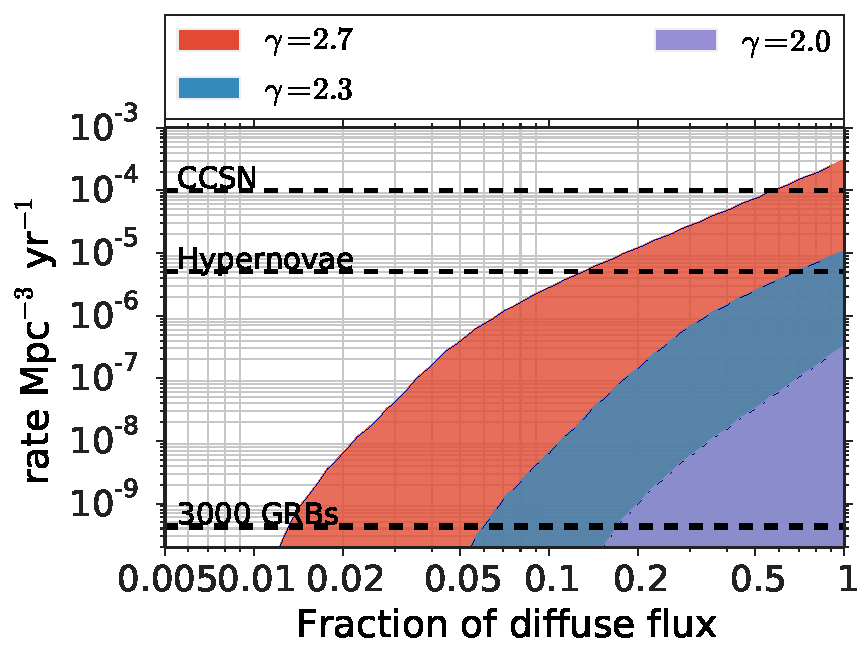
\includegraphics[width=0.75\textwidth]{fig/limits_wp_allgammas.pdf}
\caption{Limits on the contribution of short transient sources to the HESE 
flux depending on their rate density. The 90\% confidence regions are shown for 
three different spectra using the WP model.}
\label{fig:WP_2d_limit}
\end{figure}

Figure \ref{fig:WP_2d_limit} showcases the limits for the three different 
spectra using the WP model. The softer the spectrum the more singlets are 
expected especially at lower energies (Fig. \ref{fig:Espectra}) increase the 
multiplet expectation as well. Therefore, the hardest limits can be 
drawn using a spectrum with $\gamma=2.7$ decreasing in power the harder the 
spectrum gets. The results for a flux to be ruled out at a 90\% confidence 
level are listed in Table \ref{tab:WP_2d_limit_3000}.


\begin{table}[h]
  \centering
  \begin{tabular}{c|c|c}
$\gamma$  &  $N_\mathrm{GRB/yr}$ & $\zeta$ \\
\hline
2.7 & 3000 & 0.013 \\
2.3 & 3000 & 0.0595 \\
2.0 & 3000 & 0.18 \\
  \end{tabular}
  \caption{The values of the fraction to the HESE flux and the number of GRBs 
per year that are ruled out at a 90\% confidence level.}
  \label{tab:WP_2d_limit_3000}
\end{table}


\subsubsection{Signal origin}
% As part of the analysis, the question which simulated GRBs contribute most to 
% the limits, shall be answered in this section.
To answer the question on which GRBs the limits are most reliant on, the 
dependence on the luminosity and the redshift is examined at the 90\% 
confidence limit point for 3000 GRBs per year. Representing the different 
season and spectra, the BDT season and the intermediate spectrum with 
$\gamma=2.3$ were selected.

\begin{figure}[h!]
\centering
 \captionsetup{width=.9\textwidth}
%  \captionsetup{margin=0pt}
\subfloat[WP model\label{fig:ngrb_redshift_dependence_swiftdoublet_ndetF}]{%
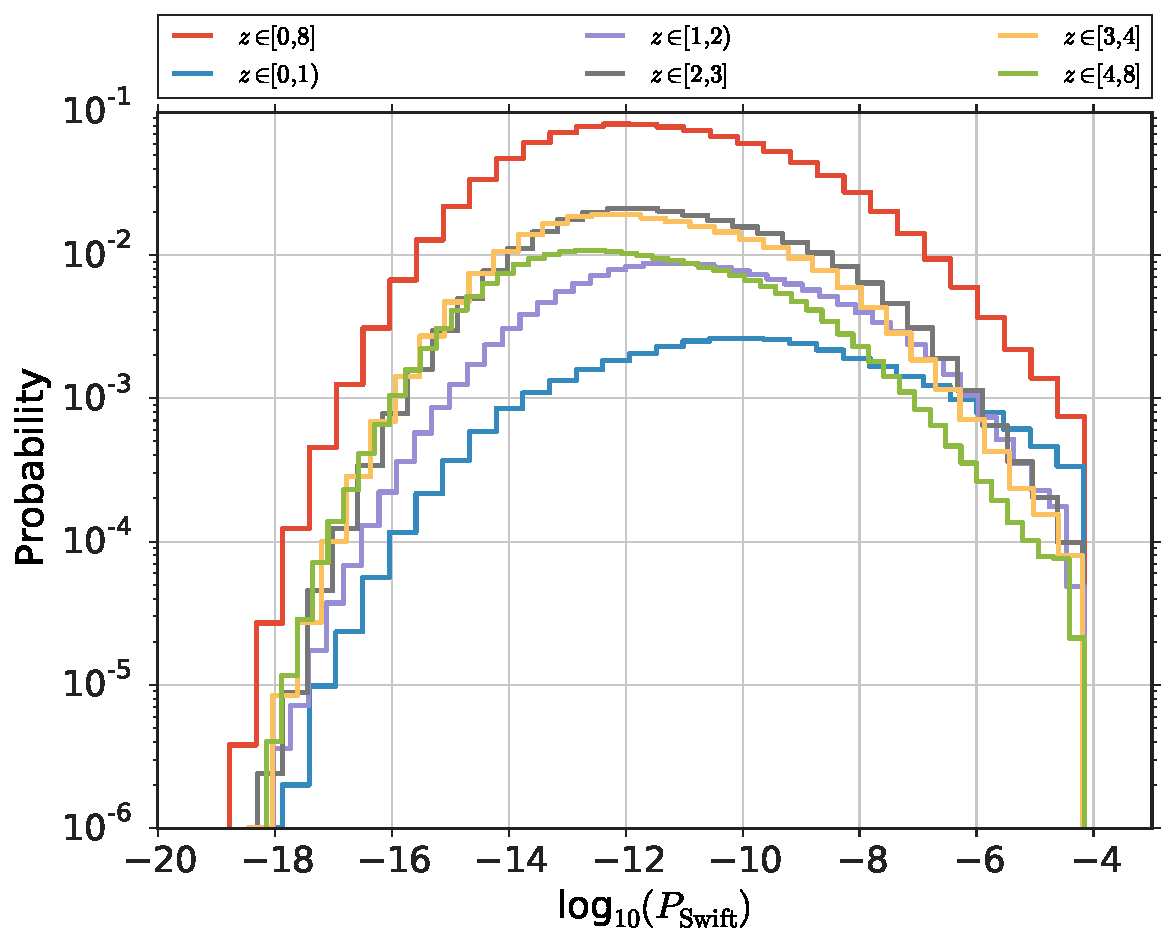
\includegraphics[width=0.45\textwidth]{%
fig/ngrb_redshift_dependence_swiftdoublet_ndetF.pdf}}
\subfloat[HC model\label{
fig:ngrb_hc_redshift_dependence_swiftdoublet_ndetF}]{%
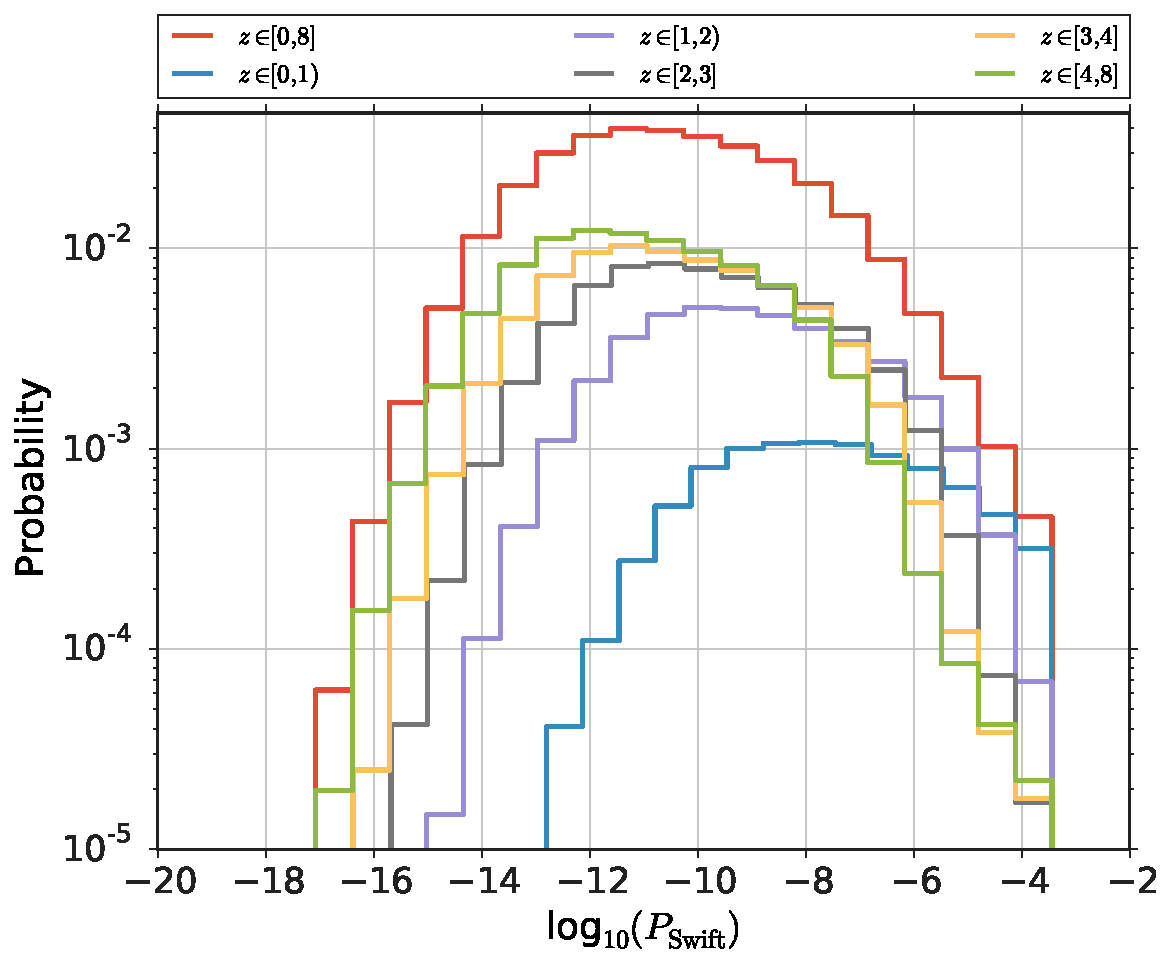
\includegraphics[width=0.45\textwidth]{%
fig/ngrb_hc_redshift_dependence_swiftdoublet_ndetF.pdf}}\\
\subfloat[WP model\label{fig:ngrb_lum_dependence_swiftdoublet_ndetF}]{%
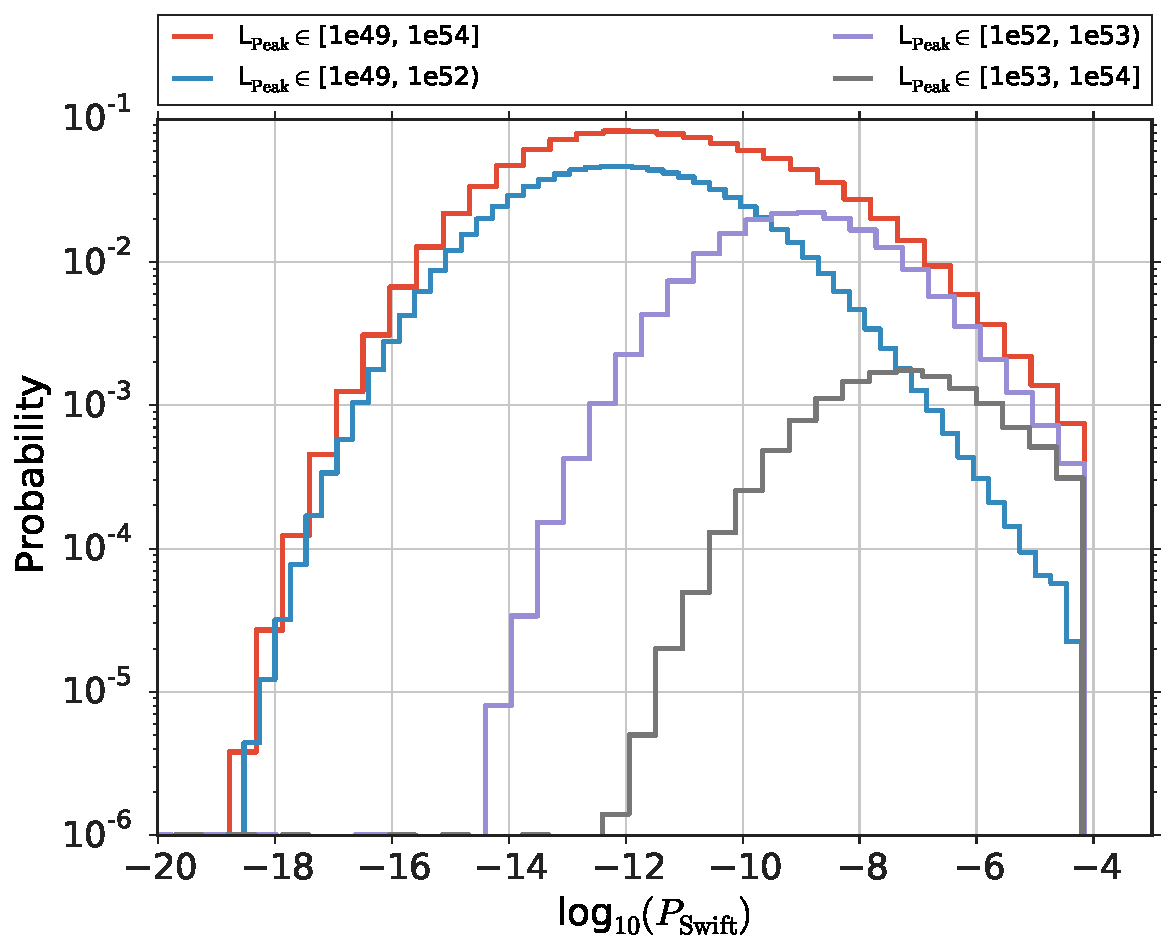
\includegraphics[width=0.45\textwidth]{%
fig/ngrb_lum_dependence_swiftdoublet_ndetF.pdf}}
\subfloat[HC model\label{fig:ngrb_hc_lum_dependence_swiftdoublet_ndetF}]{%
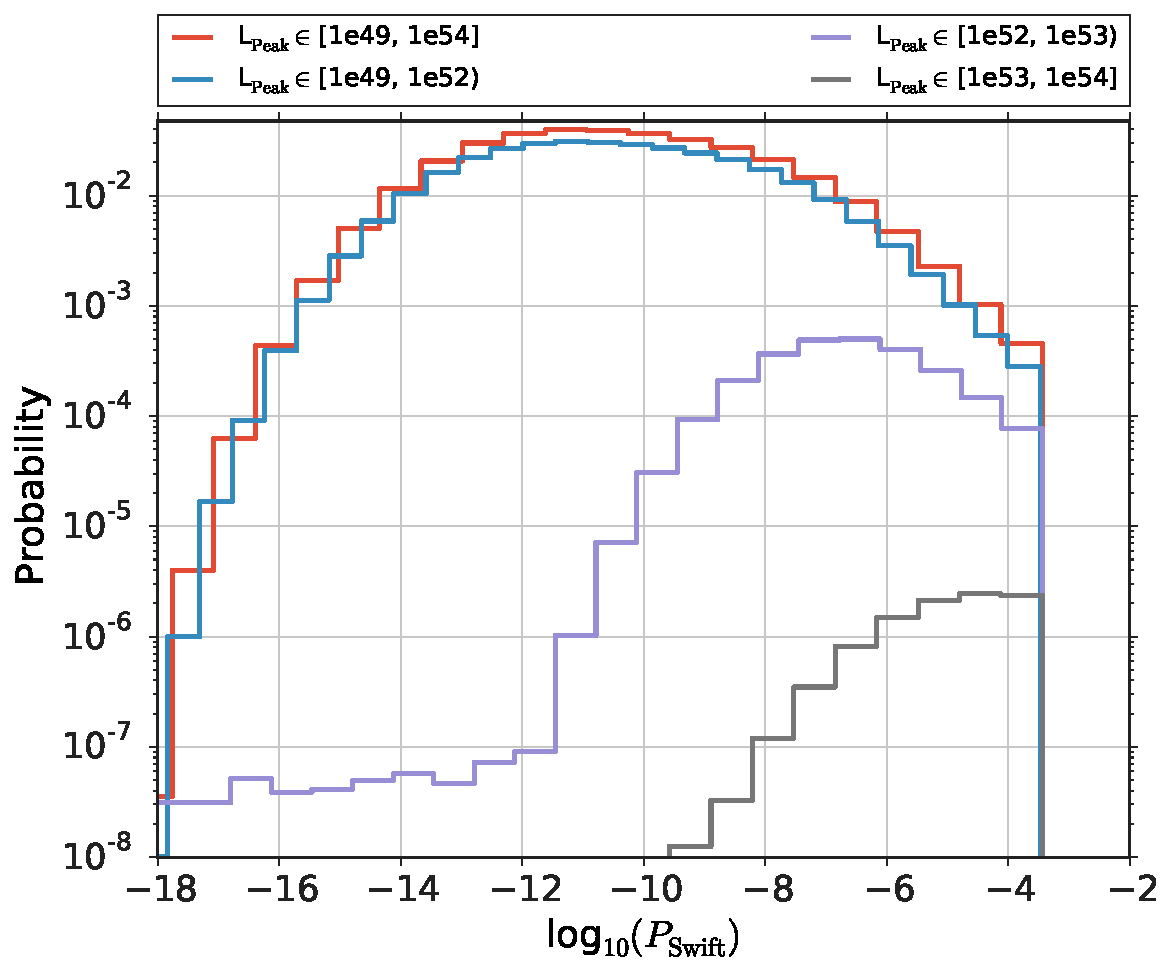
\includegraphics[width=0.45\textwidth]{%
fig/ngrb_hc_lum_dependence_swiftdoublet_ndetF.pdf}}
\caption{The probability for a GRB to have a certain probability to produce a 
Swift doublet. The contribution of the whole signal and the contribution of 
various redshift and luminosity bins are shown. Note that contributions with 
very small 
probabilities ($P_\mathrm{Swift}$) were cut off to display the more relevant 
region.}
\end{figure}

In Figure \ref{fig:ngrb_redshift_dependence_swiftdoublet_ndetF}, one can see 
the probability of a GRB to have a certain probability $P_\mathrm{Swift}$ for a 
swift doublet to be detected. Most GRBs are in a redshift range between 2 and 4 
which corresponds to the peak in the redshift distribution in Figure 
\ref{fig:GRB_rate_density}. However, these GRBs and the GRBs further out mostly 
contribute to the distribution for low to intermediate $P_\mathrm{Swift}$ 
values. The most likely GRBs to be seen in IceCube with high $P_\mathrm{Swift}$ 
values are within a redshift of one even though they occur less frequent due 
to the small volume. In total, about 0.3 GRBs per year are expected to be 
detectable with Swift doublets within the BDT season. About 35\% of which would 
be within the first redshift bin (Figure 
\ref{fig:ngrb_redshift_dependence_swiftdoublet_cum}). However, the other 
regions all contribute more than 10\% to the total signal as well.

\begin{figure}[h]
\centering
 \captionsetup{width=.9\textwidth}
%  \captionsetup{margin=0pt}
\subfloat[WP model\label{fig:ngrb_redshift_dependence_swiftdoublet_cum}]{%
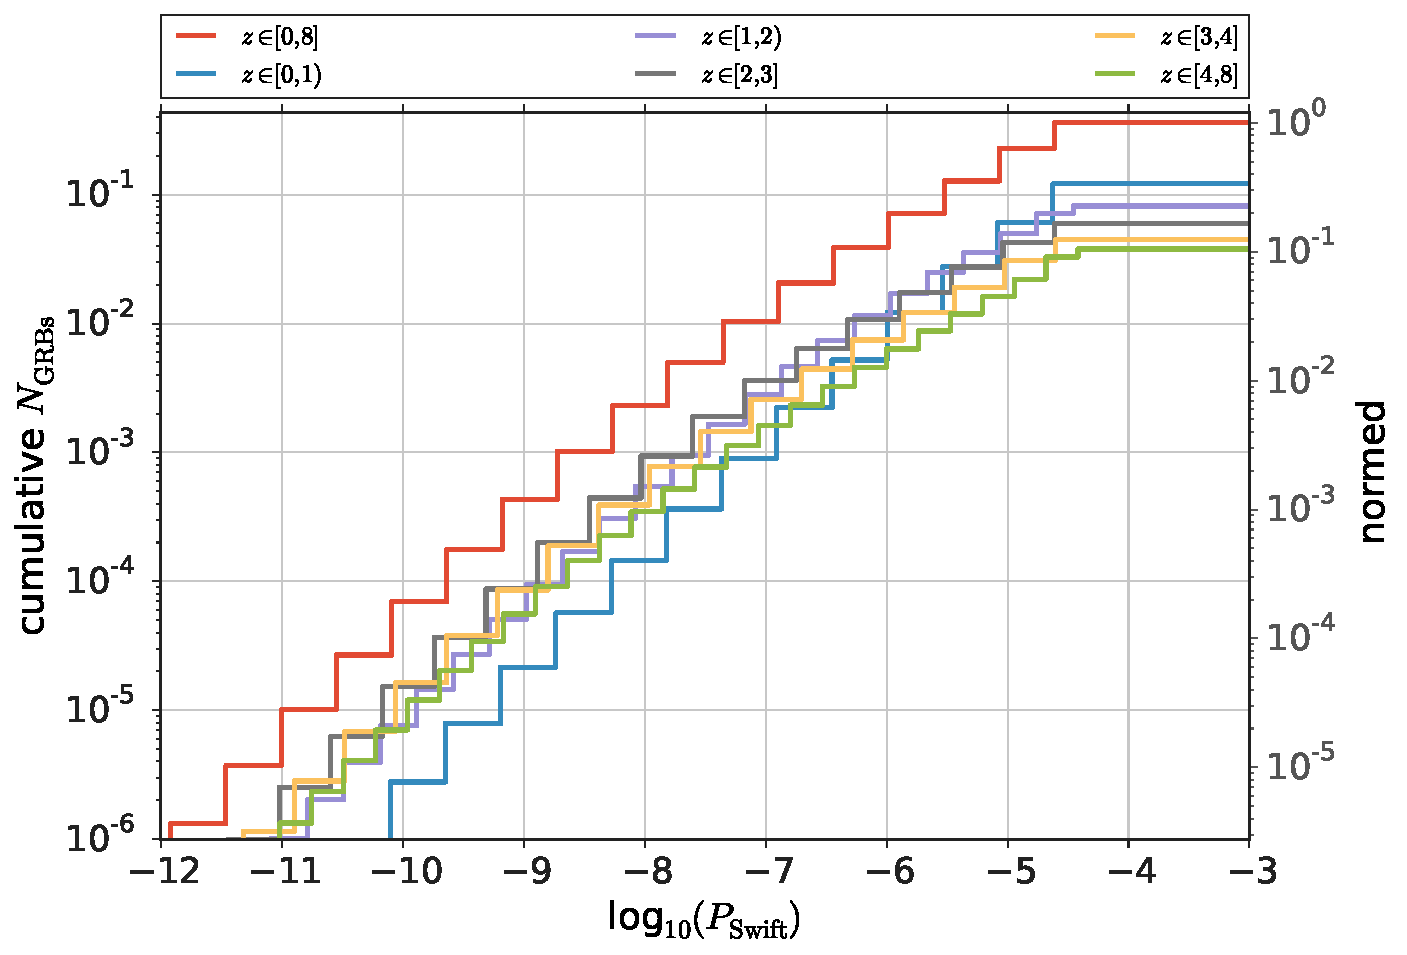
\includegraphics[width=0.45\textwidth]{%
fig/ngrb_redshift_dependence_swiftdoublet_cum.pdf}}
\subfloat[HC model\label{
fig:ngrb_hc_redshift_dependence_swiftdoublet_cum}]{%
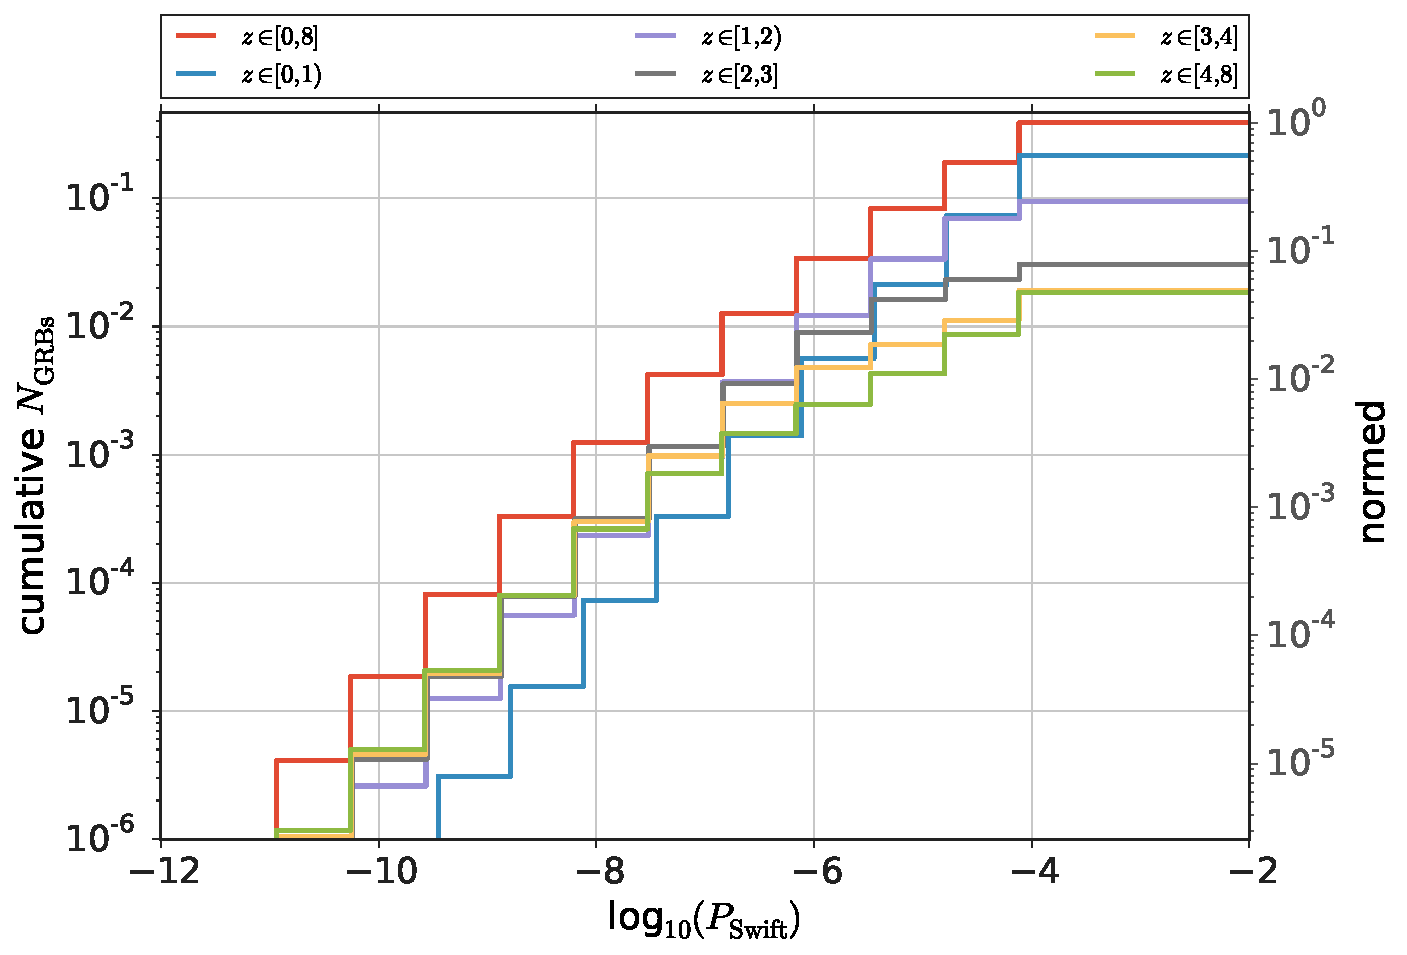
\includegraphics[width=0.45\textwidth]{%
fig/ngrb_hc_redshift_dependence_swiftdoublet_cum.pdf}}\\
\subfloat[WP model\label{fig:ngrb_lum_dependence_swiftdoublet_cum}]{%
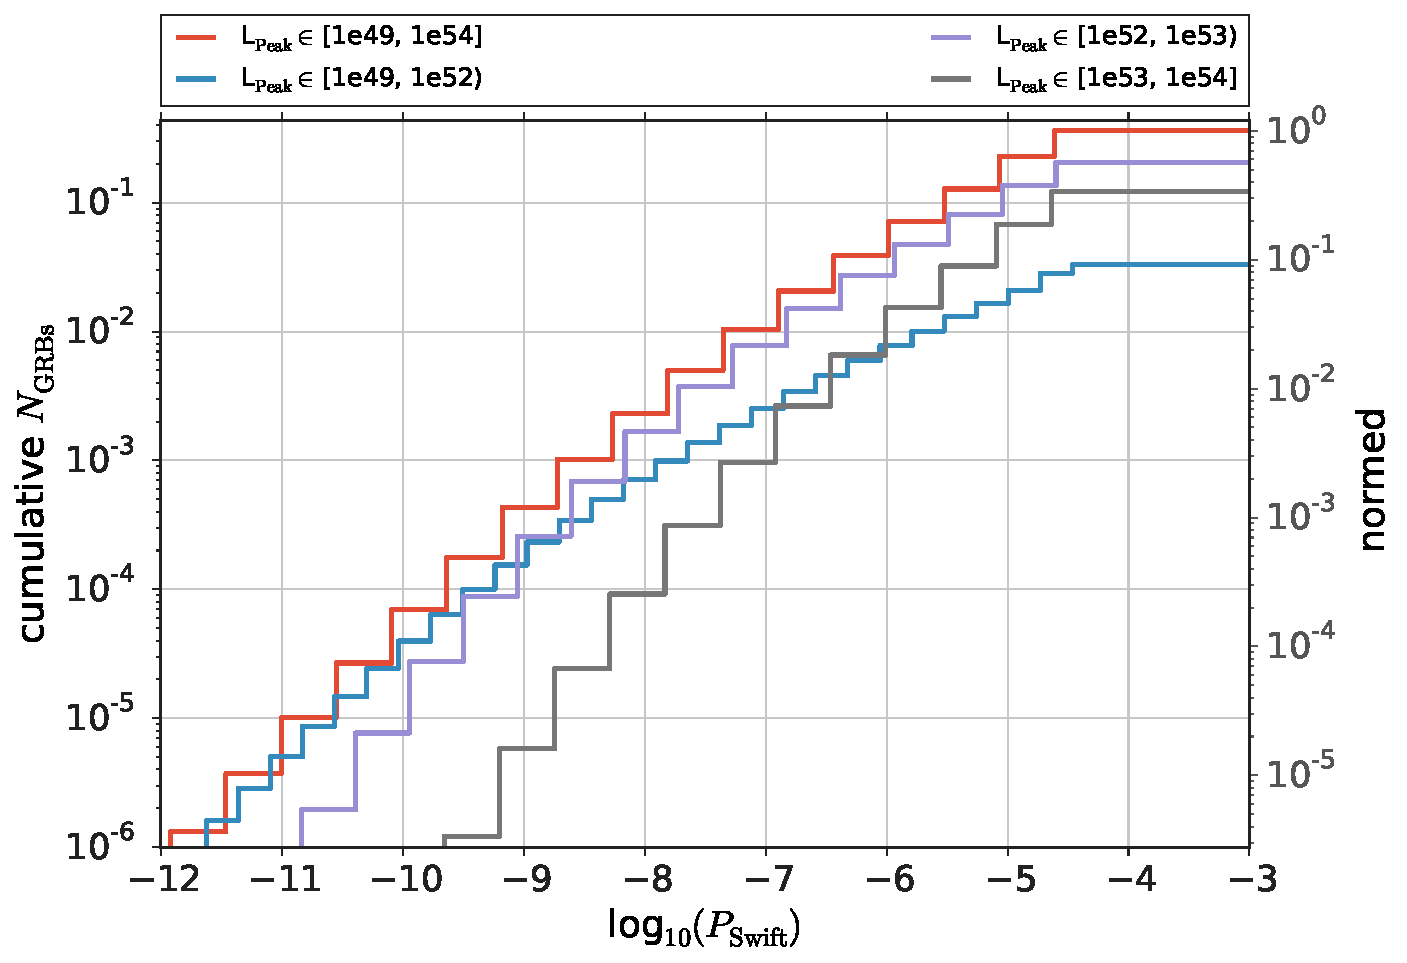
\includegraphics[width=0.45\textwidth]{%
fig/ngrb_lum_dependence_swiftdoublet_cum.pdf}}
\subfloat[HC model\label{fig:ngrb_hc_lum_dependence_swiftdoublet_cum}]{%
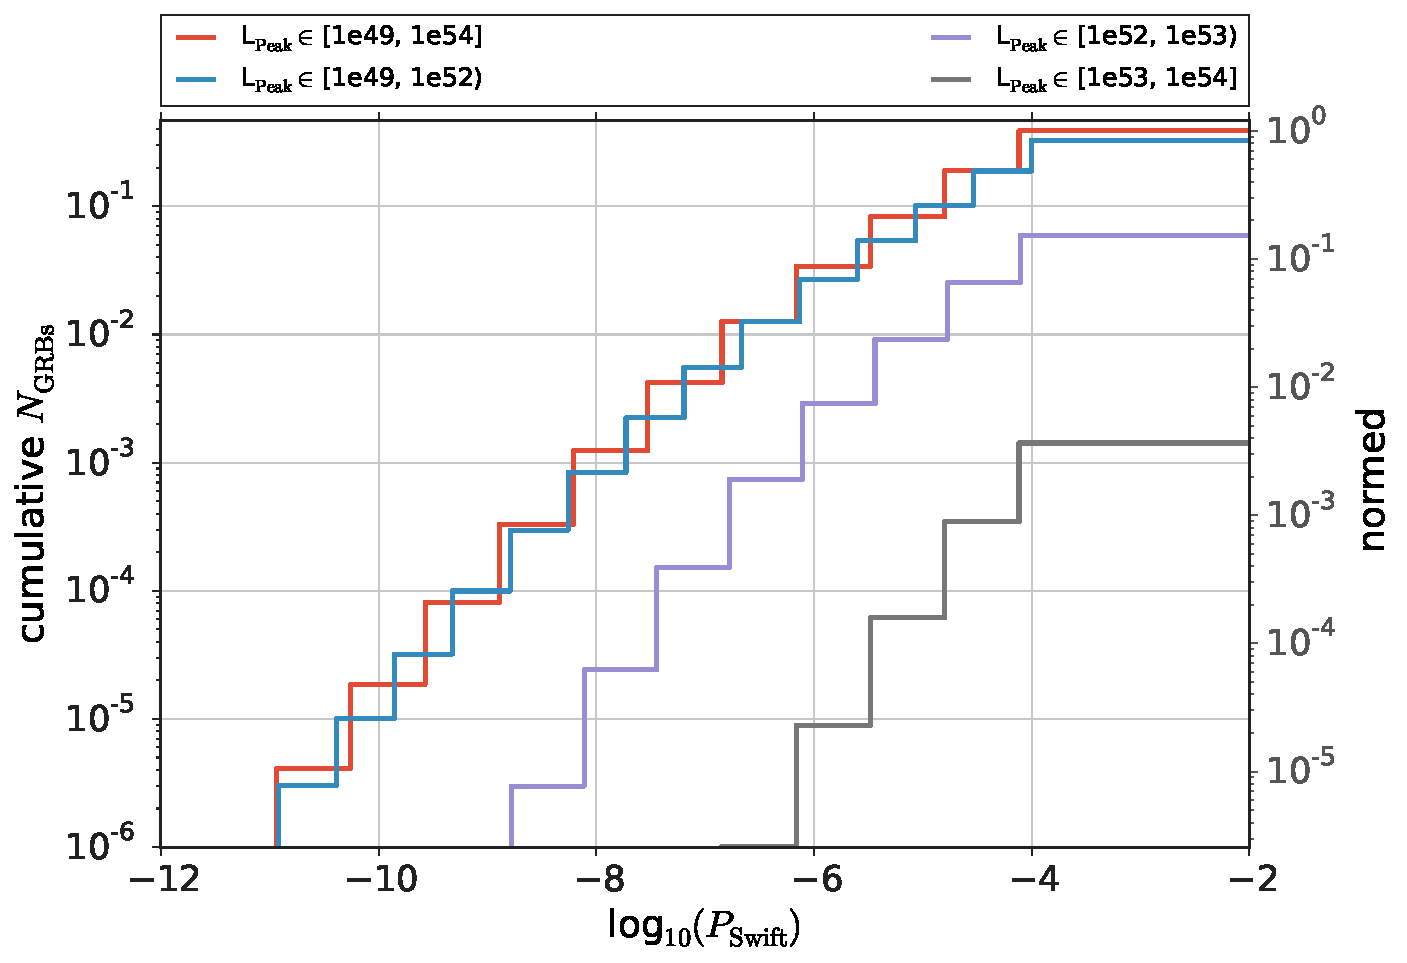
\includegraphics[width=0.45\textwidth]{%
fig/ngrb_hc_lum_dependence_swiftdoublet_cum.pdf}}
\caption{The cumulative distribution to the number of GRBs detected 
per year depending on the probability to produce a Swift doublet. The 
contribution of the whole signal and the contribution of 
various redshift and luminosity bins are shown. On the right 
y-axis, the values are divided by the complete number of GRBs produced per 
year, thus, showing the fraction contributed by the different bins. Note that 
contributions with very small 
probabilities ($P_\mathrm{Swift}$) were cut off to display the more relevant 
region.}
\end{figure}

Similar plots can be examined in Figures 
\ref{fig:ngrb_lum_dependence_swiftdoublet_ndetF} and 
\ref{fig:ngrb_lum_dependence_swiftdoublet_cum} examining the influence of the 
peak luminosity. Low luminosity GRBs of less than $10^{52}\mathrm{ erg / s}$ 
produce mainly GRBs with low detection probability only contributing about 10\% 
to the expected number of detectable GRBs. The main contribution of almost 60\% 
stems from GRBs with peak luminosities within $10^{52}$ and 
$10^{53}\mathrm{erg/s}$ by compromising between abundance and brightness. 
However, this describes the cumulative contribution of all GRBs, the most 
likely GRBs to be actually detectable are very bright and very close GRBs. 
Unfortunately, they happen rather seldom.

The same comparison can be done for the probability to see higher multiplets 
of at least three neutrinos (Figures 
\ref{fig:ngrb_redshift_dependence_multiplet_cum} and 
\ref{fig:ngrb_lum_dependence_multiplet_cum}). The signal is more dependent on 
the very bright and close GRBs as others do not produce the necessary flux to 
make a detection likely. The contribution to the total number of 0.5 detectable 
GRBs per year with the BDT season setup drops to about 6\% for the low 
luminosity GRBs while the very close GRBs up to a redshift of one constitute 
about 80\% of the total signal for higher multiplets.


\begin{figure}[h]
\centering
 \captionsetup{width=.9\textwidth}
%  \captionsetup{margin=0pt}
\subfloat[WP model\label{fig:ngrb_lum_dependence_multiplet_cum}]{%
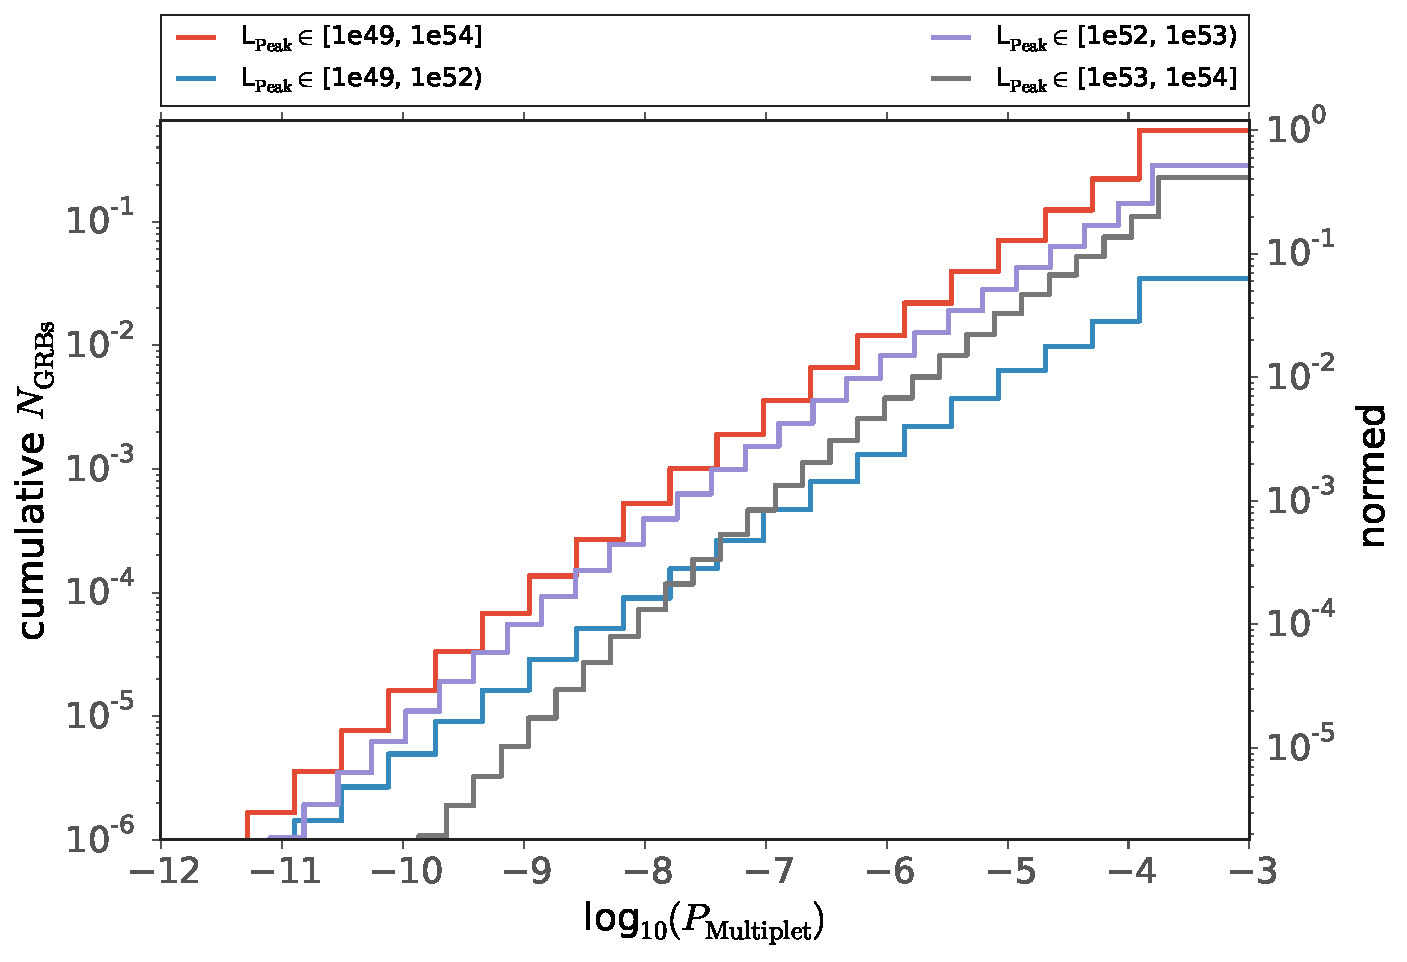
\includegraphics[width=0.45\textwidth]{%
fig/ngrb_lum_dependence_multiplet_cum.pdf}}
\subfloat[HC model\label{fig:ngrb_hc_lum_dependence_multiplet_cum}]{%
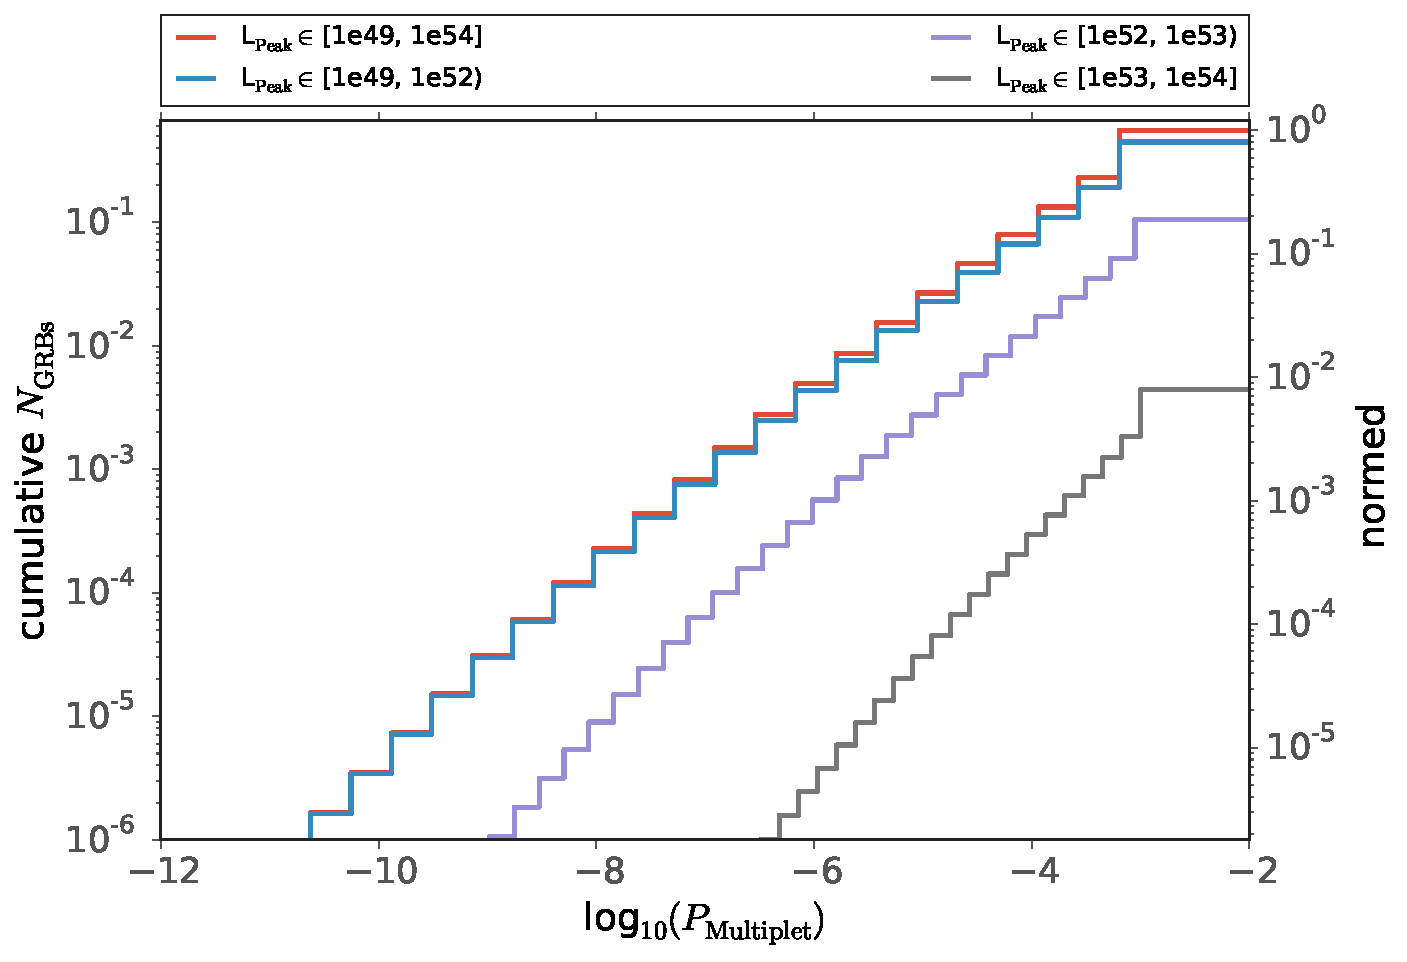
\includegraphics[width=0.45\textwidth]{%
fig/ngrb_hc_lum_dependence_multiplet_cum.pdf}}\\
\subfloat[WP model\label{fig:ngrb_redshift_dependence_multiplet_cum}]{%
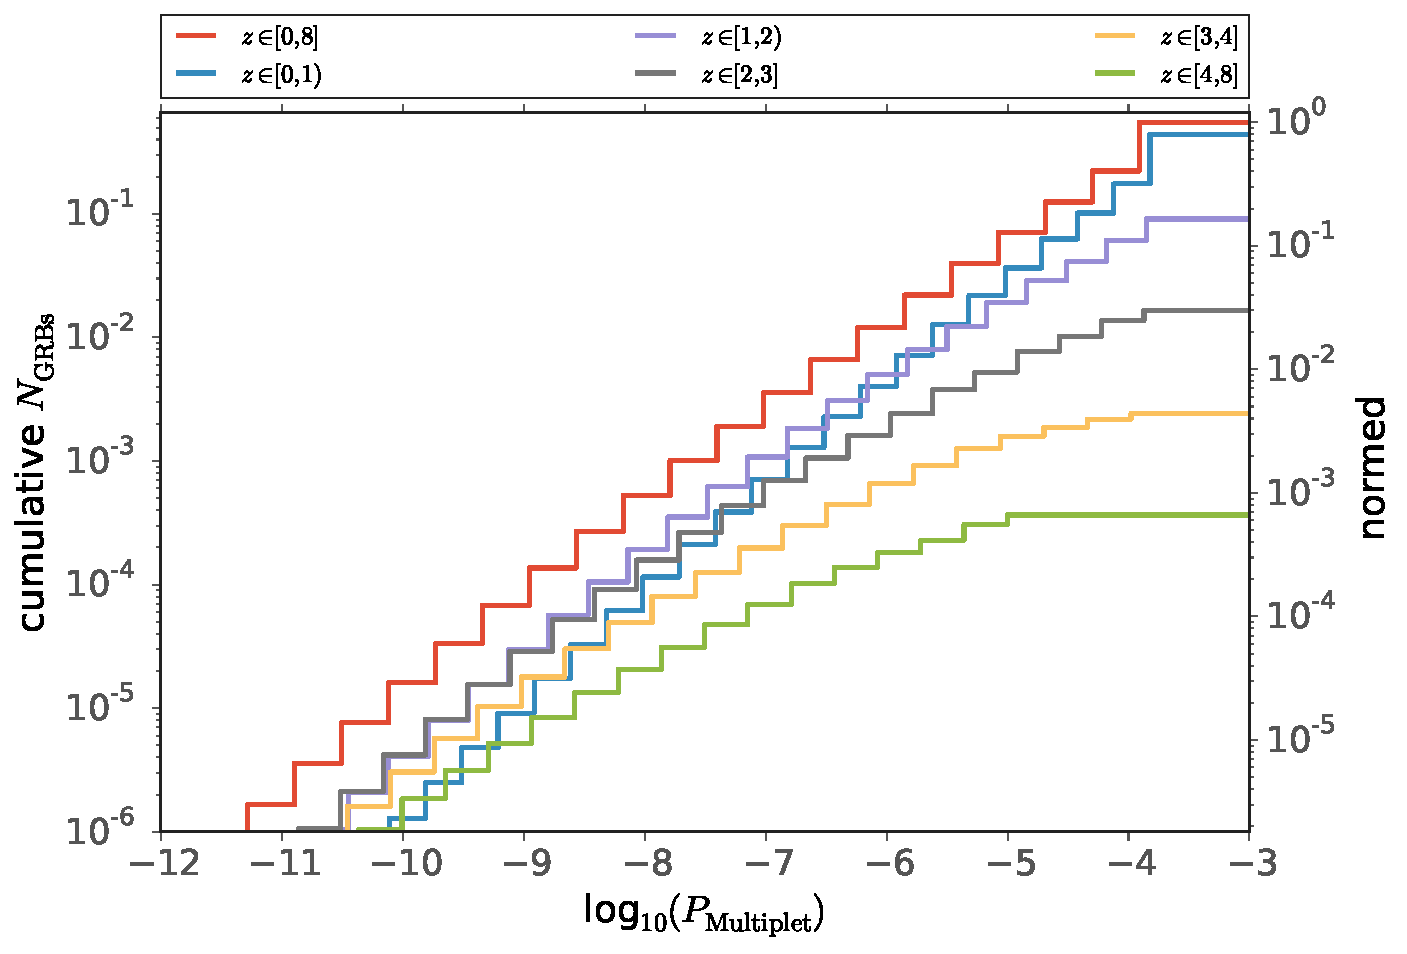
\includegraphics[width=0.45\textwidth]{%
fig/ngrb_redshift_dependence_multiplet_cum.pdf}}
\subfloat[HC model\label{fig:ngrb_hc_redshift_dependence_multiplet_cum}]{%
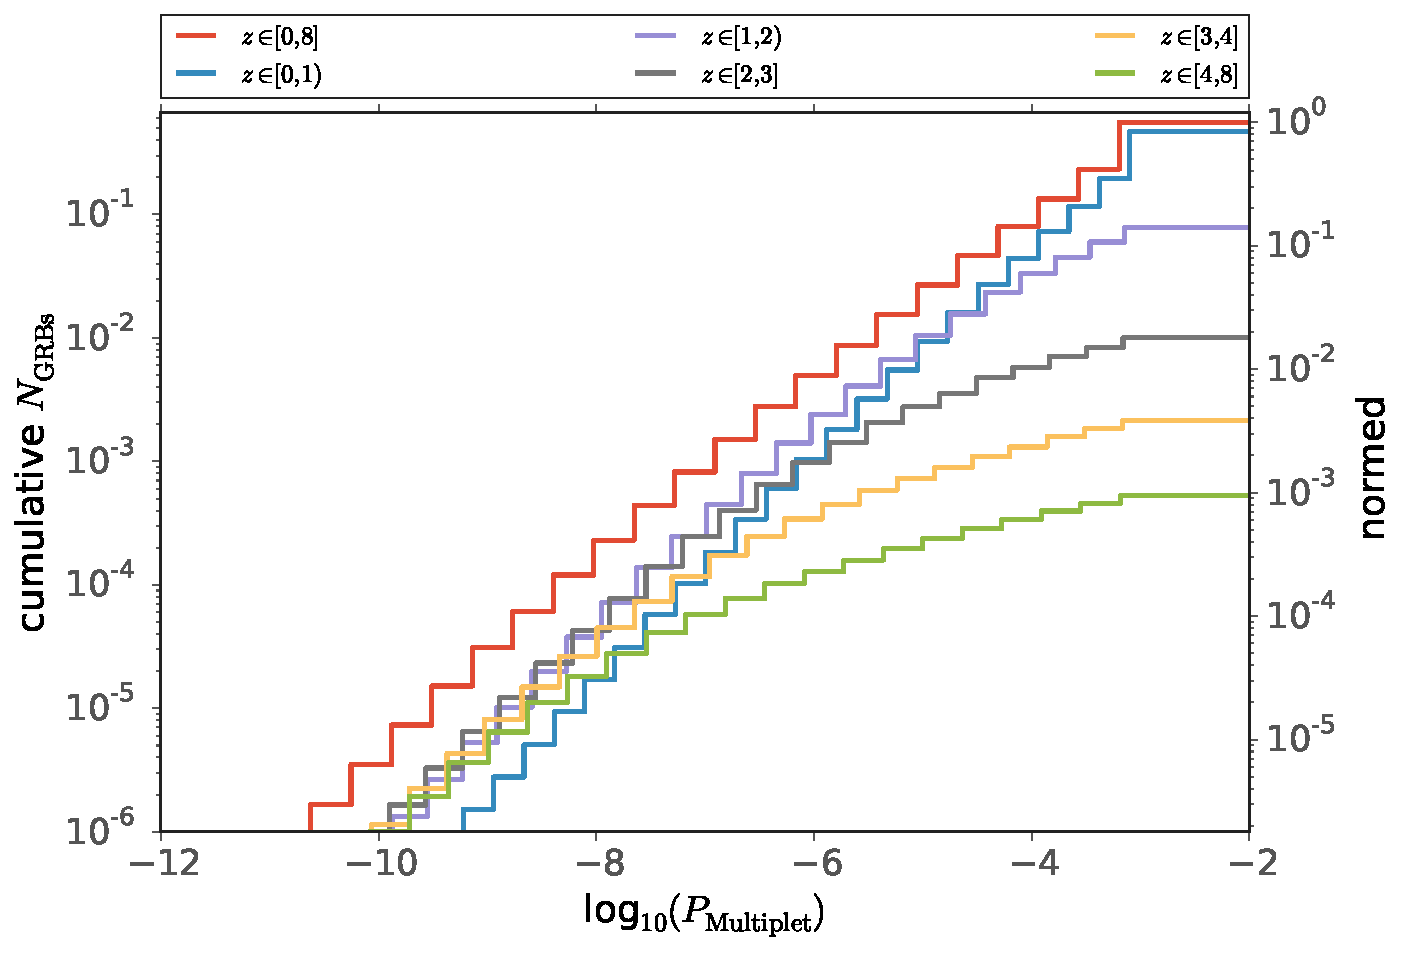
\includegraphics[width=0.45\textwidth]{%
fig/ngrb_hc_redshift_dependence_multiplet_cum.pdf}}
\caption{The cumulative distribution to the number of GRBs detected 
per year depending on the probability to produce a higher multiplet. The 
contribution of the whole signal and the contribution of 
various luminosity and redshift bins are shown. On the right 
y-axis, the values are divided by the complete number of GRBs produced per 
year, thus, showing the fraction contributed by the different bins. Note that 
contributions with very small 
probabilities ($P_\mathrm{Multiplet}$) were cut off to display the more 
relevant region.}
\end{figure}


Combining these results, one can see that we expect most signal from the 
very rare and close GRBs within a redshift of one. The number of detectable 
GRBs per year is displayed over the redshift in Figure
\ref{fig:hfcws_g2p3_n0p0595}. Both channels - the detection with swift doublets 
and higher multiplets - peak in the number of GRBs per year for GRBs within the 
first redshift bin with the multiplets dominating the signal strength. GRBs at 
these ranges produce a neutrino flux high enough that it is more likely to see 
multiplets than swift doublets. Exploring the cosmos to higher redshifts, the 
flux decreases and starting at about $z=1$ it is more likely to see swift 
doublets. However, the chance to be seen at all decreases as well, limiting the 
contribution to the cumulative signal with anything above $z=2$ only summing up 
to about 1\% of the combined multiplet and swift doublet signal. Combined with 
the fact that in contrast to the doublets there is very limited multiplet 
background, the higher multiplet channel is the main contributer to the 90\% 
confidence point for an expected 3000 GRBs per year. 

\begin{figure}[h]
\centering
 \captionsetup{width=.9\textwidth}
%  \captionsetup{margin=0pt}
\subfloat[WP model\label{fig:hfcws_g2p3_n0p0595}]{%
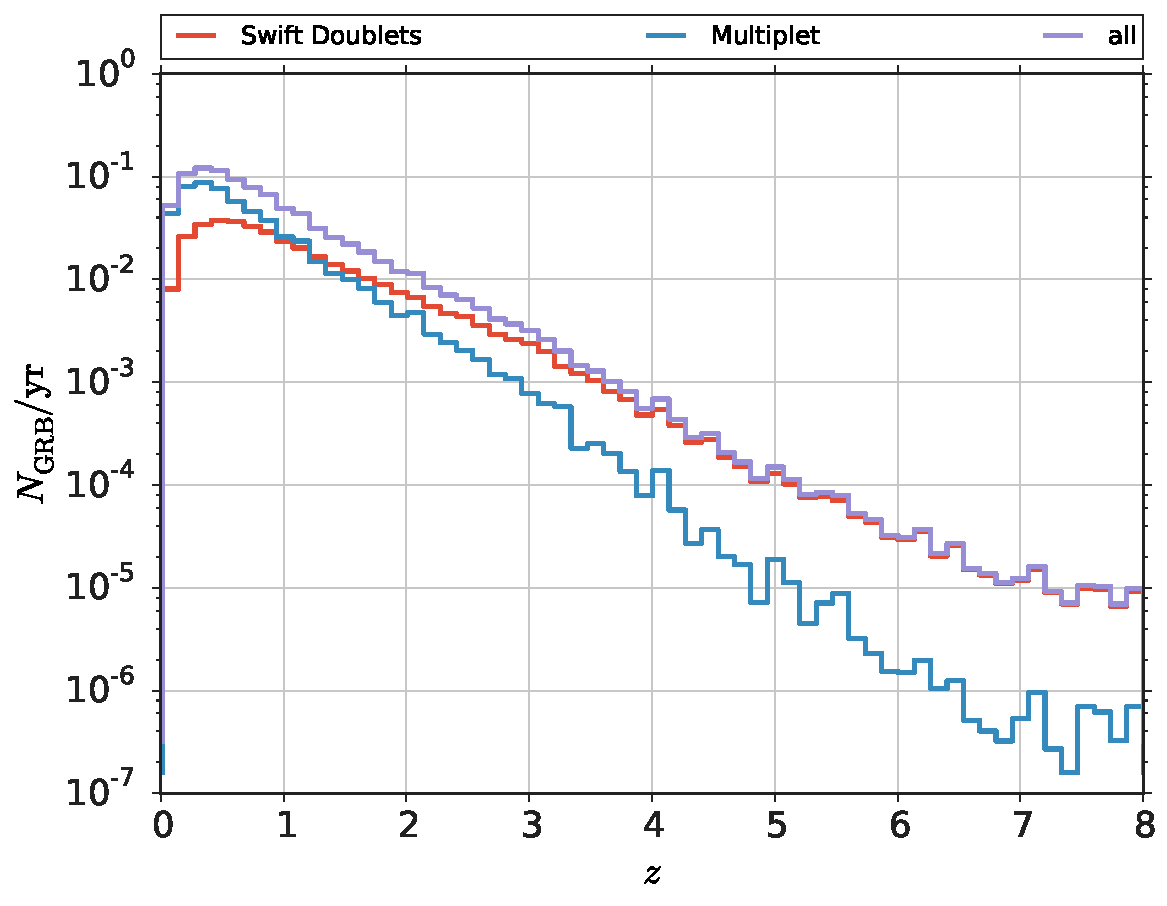
\includegraphics[width=0.45\textwidth]{%
fig/hfcws_g2p3_n0p0595.pdf}}
\subfloat[HC model\label{fig:hfcws_g2p3_hc2_n0p0759}]{%
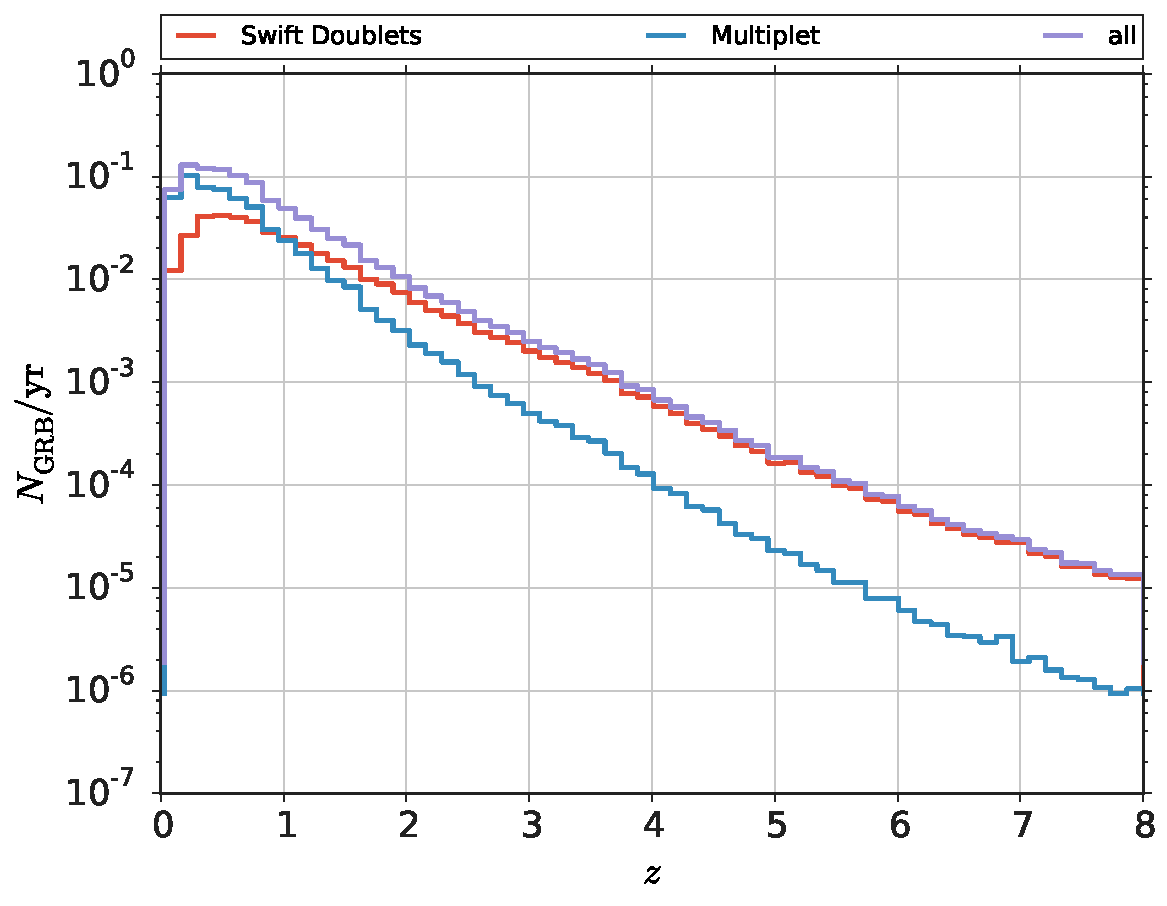
\includegraphics[width=0.45\textwidth]{%
fig/hfcws_g2p3_hc2_n0p0759.pdf}}
\caption{The cumulative distribution to the number of GRBs detected 
per year depending on the probability to produce a higher multiplet. The 
contribution of the whole signal and the contribution of 
various luminosity and redshift bins are shown. On the right 
y-axis, the values are divided by the complete number of GRBs produced per 
year, thus, showing the fraction contributed by the different bins. Note that 
contributions with very small 
probabilities ($P_\mathrm{Multiplet}$) were cut off to display the more 
relevant region.}
\end{figure}

Reducing the fraction of contribution to the HESE flux by GRBs, reduces the 
flux per GRB and as such the importance of the multiplet channel as well. A 
similar effect is to be expected by looking at higher rate densities. With more 
sources producing the same diffuse neutrino flux, the flux per source decreases.


% test statistic distribution shows the point at which p=0.9 was reached for WP 
% for 3000 GRBs showing maximum contribution of 0.05\%??? (factor 0.05 on HESE 
% flux -> $\mu$ <- describing the scaling in )
% 
% total number of GRBs is uncertain. therefore limits depending on the transient 
% rate density and the fraction of the HESE flux are drawn. the more sources 
% contribute to the known signal the less flux can be attributed to one source. 
% scale $\mu (Nexp) = \mu \frac{x GRBs}{3000 GRBs}$ . limit plots
% 
% the softer the spectrum the more singlets (especially at low energies) and 
% therefore more multiplets (reference spectrum plot) can be expected. 
% influence of a minimal energy cutoff in section ???. best limit for gamma=2.7 
% scenario. worst for gamma=2. with cutoff. some numbers (maybe in table)
% 
% looking at higher transient rates, limits extend to SN (which kind) especially 
% considering that not all SN are expected to generate jets. further discussion 
% in section ???.
% 
% where does signal come from? close and high. need to see plots to write more



\subsection{Different models}
So far, the Wanderman Piran model was examined to present the results of the
analysis. The influence of two different factors will be analyzed in the 
subsequent sections. 

The WP model is based on a broad luminosity function. The resulting variation 
in luminosity can lead to seldom but very bright GRBs producing the most 
detectable signal. Two different luminosity functions will be examined, the 
Howell Coward model (Section \ref{sec:results_HC}) and a more SN conform 
luminosity distribution (Section \ref{sec:results_SN}). 

The second factor is a low energy cut-off, having great influence on the final 
limits on the HESE flux contribution (Section \ref{sec:results_Emin}).

\subsubsection{Howell Coward}
\label{sec:results_HC}
% discripancy higher at high rates between models? at low not so much because 
% mainly dependent on multiplets and therefore close GRBs?
The Howell Coward model (Section ???) predicts various luminosity distributions 
that have one thing in common when compared to WP: less GRBs are predicted at 
high peak luminosity values (Fig. \ref{fig:wp_hc_comp_lum}). While the slope 
at 
low peak luminosities is with $\alpha_{WP}=-0.17$ and $\alpha_{HC}=-0.13$ quite 
similar, the distributions diverge quite strongly above $L_\mathrm{Peak} \geq 
1e52 \mathrm{ erg} \mathrm{ s}^{-1}$ and the HC luminosity function drops with 
$\beta{HC}=-2.42$ much faster than the WP function ($\beta{WP}=-1.44$).
% \begin{figure}[h]
% \centering
%  \captionsetup{width=.9\textwidth}
% %  \captionsetup{margin=0pt}
% \subfloat[WP model\label{fig:test_statistic_norm0p0595_rate3e3}]{%
% 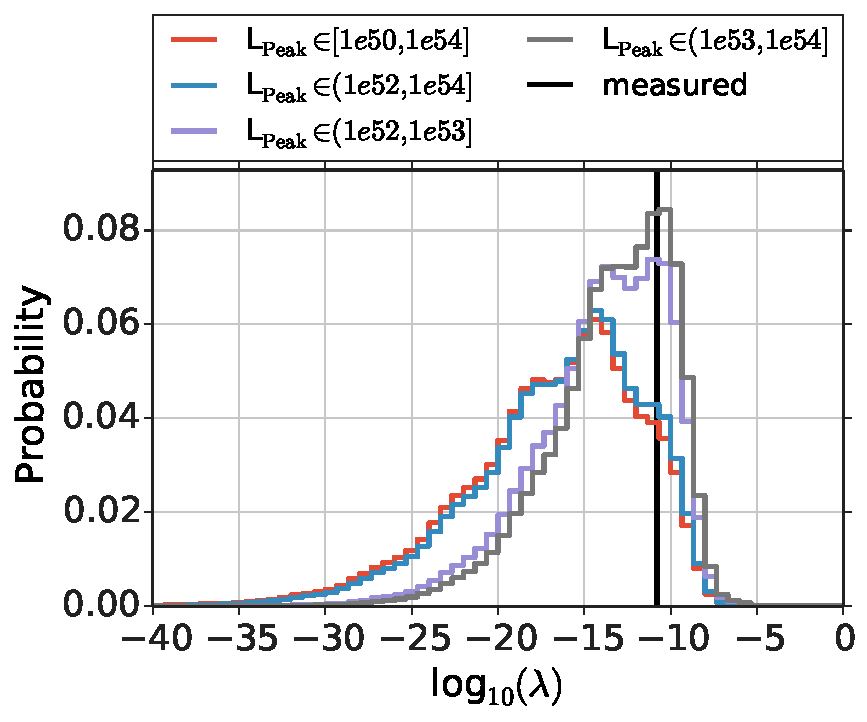
\includegraphics[width=0.45\textwidth]{%
% fig/test_statistic_norm0p0595_rate3e3.pdf}}
% \subfloat[HC model\label{fig:test_statistic_hc_norm0p0759_rate3e3}]{%
% \includegraphics[width=0.45\textwidth]{%
% fig/test_statistic_hc_norm0p0759_rate3e3.pdf}}
% \caption{caption}
% \end{figure}



The impact of this deviating behavior will be examined for the flux model with 
a spectral index of $\gamma=2.3$ as the intermediate model. The result can be 
seen in Figure \ref{fig:limits_wphc_g2p3} displaying the less 
stringent limits of the HC model. 
Assuming 3000 contributing GRBs per year, the contribution to the HESE flux of 
GRBs following the HC luminosity can be determined at a 90\% confidence level to 
be less than 7.59\% (WP: 5.95\%). This point will be examined in more detail in 
the following paragraphs.

\begin{figure}[h]
\centering
 \captionsetup{width=.9\textwidth}
%  \captionsetup{margin=0pt}
\includegraphics[width=0.75\textwidth]{%
fig/limits_wphc_g2p3.pdf}
\caption{Limits on the contribution of short transient sources to the HESE 
flux depending on their rate density. The 90\% confidence regions are shown for 
a spectrum with $\gamma=2.3$ comparing the WP and the HC model.}
\label{fig:limits_wphc_g2p3}
\end{figure}

Looking at the luminosity distribution (Fig. \ref{fig:wp_hc_comp_lum}) already 
indicates that high luminosity GRBs will have less impact for the HC model than 
the WP model as they are suppressed in frequency by almost four orders of 
magnitude at the highest luminosities of $10^{54}\mathrm{erg/s}$ alone. Figure 
\ref{fig:ngrb_hc_lum_dependence_swiftdoublet_ndetF} demonstrates that the low 
luminosity GRBs dominate the whole range of detection probabilities 
($P_\mathrm{Swift}$) even to the highest values contributing a total of about 
90\% to the cumulative swift doublet signal (Fig. 
\ref{fig:ngrb_hc_lum_dependence_swiftdoublet_cum}). The other GRBs mainly occur 
at high probability values but lack influence nonetheless due to their 
sparsity. 

Not having the abundance of bright GRBs to produce high neutrino fluxes even at 
great distances, the cumulative swift doublet signal depends with almost 60\%  
on GRBs within a redshift of one (WP: 35\%).  % \begin{figure}[h]

In case of the higher multiplets, the signal contribution is similar dependent 
on the low luminosity GRBs (Fig. 
\ref{fig:ngrb_hc_lum_dependence_multiplet_cum}) and even more so on the close 
ones (Fig. \ref{fig:ngrb_hc_redshift_dependence_multiplet_cum}). However, while 
 the behavior so far differed quite obviously from the distribution produced 
with the WP model, the possibility to detect a 
neutrino multiplet depends similarly on close by GRBs (compare Figs. 
\ref{fig:ngrb_hc_redshift_dependence_multiplet_cum} and 
\ref{fig:ngrb_redshift_dependence_multiplet_cum}). Keeping in mind that most of 
the signal is generated by multiplets within a redshift of one for both the WP 
model (Fig \ref{fig:hfcws_g2p3_n0p0595}) and the HC model (Fig. 
\ref{fig:hfcws_g2p3_hc2_n0p0759}), the comparatively small difference of a 
factor of 1.28 between the two points of 90\% confidence level assuming 3000 
GRBs per year is explained. The lack of high luminosity GRBs in the HC model 
does not matter, as the signal depends mainly on GRBs close enough to produce 
enough higher multiplets.
The discrepancy between the two models increase slightly towards higher GRB 
rate densities with less flux per GRB. While the flux decrease can be 
compensated to a degree by the high luminosity GRBs, this is not possible for 
the HC model.

% \centering
%  \captionsetup{width=.9\textwidth}
% %  \captionsetup{margin=0pt}
% \subfloat[WP model\label{
% fig:test_statistic_norm0p0595_rate3e3_cum}]{%
% \includegraphics[width=0.45\textwidth]{%
% fig/test_statistic_norm0p0595_rate3e3_cum.pdf}}
% \subfloat[HC model\label{
% fig:test_statistic_hc_norm0p0759_rate3e3_cum}]{%
% \includegraphics[width=0.45\textwidth]{%
% fig/test_statistic_hc_norm0p0759_rate3e3_cum.pdf}}
% \caption{caption}
% \end{figure}

% Looking at the test statistic distributions at the 90\% exclusion value for 
% each model, the low luminosity GRBs reproduce the overall distribution quite 
% well (Fig. ???) in case of the HC model while one can observe a significant 
% shift between the distributions - and therefore worse limits - for the WP model 
% (Fig. ???). The cumulative distributions further support the result that the 
% high luminosity GRBs do not contribute much to the HC-limit while each 
% luminosity bin ($L_\mathrm{Peak} \in [1e52, 1e53)$ and $L_\mathrm{Peak} \in 
% [1e53, 1e54]$) can still rule out the WP model at about
% 80\% confidence level.


% show contribution to Luminosity, redshift??? maybe how far can I look -> more 
% dependent on low lum GRBs. can not look as deep.

In conclusion it is possible to say that the limits for do only depend 
partially on the luminosity 
function. The limits on the HC model are mainly produced by the low 
luminosity GRBs due to the lack of high luminosity ones. This leads to 
worse limits in comparison to the WP model. However, the discrepancy is 
contained due to the dependence on multiplets from close by GRBs. Both 
models still exclude a wide 
region of parameter space.


\subsubsection{Supernova Luminosity Function}
\label{sec:results_SN}
% redshift distribution can stay the same. or did I already write that?
Examining a different luminosity distribution in the previous section was 
interesting, as a big variation of the luminosity could lead to the one very 
bright GRB to be detected. Limiting the number of high luminosity GRBs 
worsened the limits but a wide range of the parameter space could still be 
ruled out. Continuing the process one could slim down the luminosity 
distribution until only a delta function remains. The SN luminosity function 
(Eq. ???) is a step in that direction with a Gaussian with width ???. The 
average luminosity is higher than a lot of values from the WP or HC models, 
however, it is very unlikely to have GRBs with very high luminosities.

SNe are especially interesting because using the WP model and a spectrum with 
$\gamma=2.7$, the limits extend from rate densities that are likely for GRBs to 
very high values and reaching the population of Core Collapse SNe. According to 
???, some SNe could create jets similar to GRBs producing high energy 
neutrinos. Considering that not all SNe might have a jet and that we could only 
see them if the jet pointed towards earth, one has to look at the parameter 
space at possibly a hundredth or less than the actual SN rate density making 
the limits even more stringent. Using the same redshift distribution as 
motivated in Section ??? and the luminosity distribution (Eq. ???) chosen to 
represent the SNe population, the limits worsen but still exclude the 
possibility that SNe contribute the complete measured high energy neutrino 
flux (Fig. \ref{fig:limits_wpsn_g2p7}). However, this depends on choosing the 
most optimistic fit to the measured HESE flux with $\gamma=2.7$ (Eq. ???). 
Using a harder spectrum decreases the chance of ruling out SNe as the main 
source.

\begin{figure}[h]
\centering
 \captionsetup{width=.9\textwidth}
%  \captionsetup{margin=0pt}
\includegraphics[width=0.75\textwidth]{%
fig/limits_wpsn_g2p7.pdf}
\caption{Limits on the contribution of short transient sources to the HESE 
flux depending on their rate density. The 90\% confidence regions are shown for 
a spectrum with $\gamma=2.7$ comparing the WP model to a more SN like 
luminosity distribution.}
\label{fig:limits_wpsn_g2p7}
\end{figure}

\subsubsection{Low Energy Cut-Off}
\label{sec:results_Emin}
This section examines the influence low energy cut-off, the minimal energy 
neutrinos have at source (Eq. ???) that arises in the flux calculation (Eq. 
???). As explained in section ???, the absolute normalization of the flux does 
not change but stays the same when using the same spectrum. However, if the 
cut-off is high enough, no low energy neutrino is available to form multiplets 
reducing the likelihood of detection. 

The lowest measured energy of the HESE events was 30 TeV. Setting 
$\hat{E}_\mathrm{min}$ to 100 TeV, no OFU singlet with energies lower than ??? 
GeV should contribute (??? line in Fig. ???). The impact on the signal is more 
pronounced for the softer spectra, as they predict more events at lower 
energies (Fig. ???). Using the spectrum with $\gamma=2.3$, the limits worsen 
drastically and are in the range of the spectrum with $\gamma=2$ with an 
exponential cut-off (Fig. \ref{fig:limits_wp_g2p3_g2p0_Emin100e3}). 

% word about should be same for E-2 as OFU spectra are not that different above 
% that energy


\begin{figure}[h]
\centering
 \captionsetup{width=.9\textwidth}
%  \captionsetup{margin=0pt}
\includegraphics[width=0.75\textwidth]{%
fig/limits_wp_g2p3_g2p0_Emin100e3.pdf}
\caption{Limits on the contribution of short transient sources to the HESE 
flux depending on their rate density. The 90\% confidence regions are shown for 
a spectrum with $\gamma=2.3$ and $\gamma=2$ comparing them to a spectrum with 
$\gamma=2.3$ and a minimal neutrino energy at source of 100 TeV.}
\label{fig:limits_wp_g2p3_g2p0_Emin100e3}
\end{figure}



% \section{Discussion}

% \section{}
\bibliographystyle{plain}
\bibliography{references}

\end{document}
